\documentclass[british,         % thesis language
% ngerman
BCOR=2mm,                       % binding correction for printing (ca. 1mm per 10 pages for hardcover binding)
11pt,                           % font size
a4paper,						% page layout
oneside,						% oneside/twoside option for printing
cdgeometry=centered,            % setting of page geometry (format, height, page margins; set to 'cdgeometry=false' for individual type area calculation by package 'typearea'
toc=chapterentrydotfill,        % dots in table of contents
toc=indent,                     % indentation of toc items
bibliography=totoc,         	% bibliography to table of contents
listof=totoc,                   % lists to table of contents
numbers=noenddot,				% last number in table of contents without dot
parskip=full,                   % line break with a free line
cdfont=true
%cdmath=false					% regular font in math mode
]{tudscrreprt}                  % document class ('tudscrreprt' in most cases)

\headlogo[]{figures/EE2_logo.png}
\iftutex
\usepackage{fontspec}
\else
\usepackage[T1]{fontenc}
\usepackage[ngerman=ngerman-x-latest]{hyphsubst}
\fi
\usepackage{isodate}

%% ****************************************************************
%% Packages
%% ****************************************************************

% basic packages

%% set language (german or english)
%% Note that the choice of language for babel only determines the language of chapter titles and paper formalia which are defined in the tudscr package.
%\usepackage[ngerman]{babel}
\usepackage[british]{babel}

\usepackage{geometry}                       % definition of individual page style/geometry
\usepackage{setspace}                   	% line spacing 
\usepackage{enumitem}	                    % enumerations
\usepackage[hyphens]{url}                   % line break at a slash in urls
\usepackage[headsepline]{scrlayer-scrpage}  % head and foot notes
\usepackage{mathptmx}                       % sets Times New Roman for math
\usepackage{amsmath}                        % mathematical equations
%\setlength\mathindent{0pt}
\usepackage[gen]{eurosym}                   % for € symbol
\usepackage{microtype}                      % for several typographical details
\usepackage[pdfborder={0 0 0}]{hyperref}    % for links in the document
\usepackage[output-decimal-marker={.}]{siunitx} % definition of units, displayed with decimal point; may change decimal separator to "," for german language
\usepackage[nohyperlinks]{acronym}	        % for abbreviations list and makros
\usepackage{listings}                       % for code listings
\usepackage{xcolor}                         % definition of colors for highlighting, drawings, ...
\definecolor{codegray}{rgb}{0.5,0.5,0.5}    % background color for code listings
\usepackage{scrhack}                        % avoids warnings for deprecated packages

% packages for tables and graphics
\usepackage{circledsteps}
\usepackage{placeins}
\usepackage{graphicx}                       % import of graphical elements (png, pdf, ...)
\usepackage{hvfloat}	                    % rotating tables and pictures
\usepackage[countmax]{subfloat}             % arrangement of two tables/figures in one environment
\usepackage{here}
\usepackage{multirow}                       
\usepackage{multicol}      
\usepackage{tabularx}
\usepackage{diagbox}
\usepackage{makecell}
\usepackage{colortbl}
\usepackage{threeparttable}

%\usepackage{showframe}                     % displays page margins, ...

\newcolumntype{C}[1]{>{\centering\arraybackslash}m{#1}} % new centered column type
\newcolumntype{L}[1]{>{\arraybackslash}m{#1}}

\usepackage[labelfont=bf, singlelinecheck=off]{caption} % global settings for figure and table captions
\captionsetup[figure]{justification=raggedright}
\captionsetup[table]{justification=raggedright}
\DeclareCaptionType{listing}[Listings][List of Listings] % definition of new environment with title for toc




%% ****************************************************************
%% Page and font settings
%% ****************************************************************
% normal spacing between items of enumerations
\setlist{noitemsep}

% URLs keep the same font
\urlstyle{same} 

% change name of toc according to thesis language
\addto\captionsbritish{
	\renewcommand{\contentsname}
	{Table of Contents}
}
\addto\captionsngerman{
	\renewcommand{\contentsname}
	{Inhaltsverzeichnis}
}

% set the titles of chapters etc. to the same font like chosen for the content
\setkomafont{chapter}{\normalfont\huge\bfseries}
\addtokomafont{section}{\normalfont\Large\bfseries}
\addtokomafont{subsection}{\normalfont\large\bfseries}
\addtokomafont{subsubsection}{\normalfont\bfseries}
\addtokomafont{paragraph}{\normalfont\bfseries}
\addtokomafont{chapterentry}{\normalfont}
\addtokomafont{disposition}{\setstretch{1}}


% global settings for spacing around headlines
\RedeclareSectionCommand[
%runin=false,
afterindent=false,
beforeskip=\baselineskip,
afterskip=.1em]{section}

\RedeclareSectionCommand[
%runin=false,w
afterindent=false,
beforeskip=0.5\baselineskip,
afterskip=.1em]{subsection}


% set individual page style with header and footer
\pagestyle{scrheadings} 
\clearpairofpagestyles
\ohead{\headmark}
\automark[section]{chapter}     % chapter title in page header
\ofoot[\pagemark]{\pagemark}    % page number in footer
\renewcommand*\chapterpagestyle{scrheadings}    % header on first page of a chapter 
\renewcommand*\chaptermarkformat{}  % removes chapter number from header


%% my stuff
\usepackage{csquotes}
\usepackage{chemformula}
\usepackage{blindtext}
\usepackage{hyperref}
\usepackage[
backend=biber,
style=numeric,
sorting=ynt
]{biblatex}

\addbibresource{researchProject.bib}
\usepackage{graphicx} % Required for inserting images
\usepackage{setspace}
\usepackage{float}
\usepackage{todonotes}
\usepackage{amsmath}

\usepackage{todonotes}
\setlength {\marginparwidth }{2cm}



\title{Research Project}
\author{Sebastian Trümper}
\date{February 2025}

\begin{document}
\listoftodos
\doublespacing

%% change terms to english/german as necessary
\faculty{Fakultät Wirtschaftswissenschaften}
\chair{Professur für BWL, insbesondere Energiewirtschaft}
\date{30.03.2025}
\title{%
	Optimizing Strategies for battery storages in combination with renewable energy production facility
	at the German aFFr/DA markets
}
%% set subject/paper type (seminar, bachelor, master, diploma, diss) and graduation
\subject{Research Project}
%\graduation[M.Sc.]{Master of Science}

\newcommand{\authorsName}{Sebastian Trümper}


%\newcommand{\authorsNameC}{Max MustermannC}
%\newcommand{\authorsNameD}{Max MustermannD}

%% name each author following the pattern given below
\author{%
	\authorsName%
	\matriculationnumber{3631139}%
	\dateofbirth{13.09.1990} %
	\placeofbirth{Naumburg}%
}

%\matriculationyear{2010} %% not necessary

%% name of seminar/thesis supervisor(s)
\supervisor{Dr. Hannes Hobbie, Margrit Wicke, Dr. Christoph Zöphel} %% name of your academic supervisor
\maketitle

\pagenumbering{Roman} %% roman page numbers for abstract, toc, indexes, ...
\setcounter{page}{1}

%% sets 1.5 line spacing
\setstretch{1.5}
\setlength{\footheight}{20.40001pt} %% commonly not necessary, but prevents scrpage errors
\setlength{\headheight}{20.40001pt} %% commonly not necessary

%% sensible spacing around chapter headlines
%% changes to presets not recommended
\renewcommand\chapterheadstartvskip{\vspace*{-40pt}}
\renewcommand\chapterheadendvskip{\vspace*{11pt}}

%% inclusion of abstract file
%% either with tudscr makro (in german version the name of the first page would be "Zusammenfassung") or as single file with page stlye
%% adjust file chapters/abstract accordingly
\TUDoption{abstract}{single, chapter}

\begin{abstract}
	abstract
\end{abstract}


\tableofcontents

\chapter*{Sets \& Variables \& Parameters}
\todo{sauber und ausführlich machen }
\todo{alle tabellen nochmal korrektur lesen }
\todo{make tables look nice}
\todo{eventuell table heads dick machen}
\textbf{Abbreviations}
\begin{table}[!h]
	\begin{tabular}{c|c}
		Abbreviations & Description                                                                            \\
		\hline
		aFRR          & automatic Frequency Restoration Reserve                                                \\
		GAMS          & General Algebraic Modeling System                                                      \\
		TSO           & transmission system operators                                                          \\
		CBMP          & grenzüberschreitenden Grenzpreis                                                       \\
		ARIMA         & Autoregressive Integrated Moving Average                                               \\
		SARIMA        & Seasonal Autoregressive Integrated Moving Average                                      \\
		TBATS         & Trigonometric seasonality Box-Cox transformation ARMA errors Trend Seasonal components \\
	\end{tabular}
\end{table}\\

Groß geschriebene Variablen werden endogen ermittelt. Klein geschriebene Variablen werden exogen vorgeschrieben.\\

\begin{tabular}{c|c|c}
	Variable       & Description                                                                                                      \\
	\hline
	$RL$           & Regelleistungsmarkt                                                                                              \\
	$DA$           & Day Ahead Markt                                                                                                  \\
	$RA$           & Regelarbeitsmarkt                                                                                                \\
	$Q^i_{y}$      & Gebotsmenge der Art i(=in/out) am Markt y                                                                        \\
	($X^i_{y})$    & (lineare Gebotsmenge der Art i(=in/out) am Markt y)                                                              \\
	$P^i_{y}$      & Gebotspreis der Art i(=in/out) am Markt y                                                                        \\
	$E^{in}_{DA}$  & $EnergyInDA(t)$                                                                   & energy in day ahead market   \\
	$E^{out}_{DA}$ & $EnergyOutDA(t)$                                                                  & energy out day ahead market  \\
	$E^{in}_{RT}$  & $EnergyInRT(t)$                                                                   & energy in real time market   \\
	$E^{out}_{RT}$ & $EnergyOutRT(t)$                                                                  & energy out  real time market \\
	$ER$           & emergency reload
	$B^i_y$        & Binäre Variable die den Zuschlag (B=1) der Art i(=in/out) am Markt y signalisiert                                \\
	\label{tab:my_label}                                                                                                              \\
\end{tabular}
\\

\todo{entweder überall gams äquivalnt ergänzen oder überall weg lassen}
\textbf{Parameter}
\begin{table}
	\centering
	\begin{tabular}{c|c|c}
		Parameter               & GAMS Equivalent                                                   & Description                        \\
		\hline
		$f_{DA}$                & $priceForeCastDA(t)$                                              & forecast price day ahead market    \\
		$f_{RT}$                & $priceForeCastRT(t)$                                              & forecast price real time market    \\

		$p_{DA}$                & $ priceProbDA $                                                   & probability for price $p_{DA}$     \\
		$p_{RT}$                & $ priceProbRT $                                                   & probability for price $p_{RT}$     \\


		$r$                     & Rate mit der der Stromspeicher geladen/entladen werden kann                                            \\
		$a$                     & Anschlusskapazität                                                                                     \\
		$z^{in}(t)$             & $binaryInDA(t)$                                                   & binary variable if bid is accepted \\
		$z^{out}(t)$            & $binaryOutDA(t)$                                                  & binary variable if bid is accepted \\
		$\omega_{DA}(pDA) $     & Wahrscheinlichkeit für Zuschlag bei Preis $P_{DA}$                                                     \\
		$\omega^i_{y}(P^i_{y})$ & Gebotswahrscheinlichkeit für $P^i_{y}$                                                                 \\
		$p^i_{y}(s^i_y)$        & Gebotspreis der Art i(=in/out) am Markt y für Szenario $s^i_y$                                         \\
		$\omega^i_{y}(s^i_y)$   & Gebotswahrscheinlichkeit für entsprechendes Preisszenario $s^i_y$                                      \\
		$c^i_y$                 & Marktclearingpreis der Art i(=in/out) am Markt y                                                       \\
		$m$                     & eine sehr große Zahl                                                                                   \\
	\end{tabular}
	\caption{Variables}
	\label{tab:my_label}
\end{table}





\textbf{Variables - simplified model + wind park}

\begin{table}[]
	\doublespacing
	\centering
	\begin{tabular}{c|c|c}
		Parameter        & GAMS                             & Description                     \\
		$f_{DA}$         & $priceForeCastDA(t)$             & forecast price day ahead market \\
		$f_{RT}$         & $priceForeCastRT(t)$             & forecast price real time market \\

		$E^{in}_{DA}$    & $EnergyInDA(t)$                  & energy in day ahead market      \\
		$E^{out}_{DA}$   & $EnergyOutDA(t)$                 & energy out day ahead market     \\

		$E^{in}_{RT}$    & $EnergyInRT(t)$                  & energy in real time market      \\
		$E^{out}_{RT}$   & $EnergyOutRT(t)$                 & energy out  real time market    \\

		$E^{in}_{stor}$  & $$                               &                                 \\
		$E^{out}_{stor}$ & $$                               &                                 \\
		$p^+_{WP}$       & costs of emergency working point
		$p^-_{WP}$       & costs of emergency working point
	\end{tabular}
	\caption{Variables}
	\label{tab:my_label}
\end{table}

\begin{table}
	\begin{tabular}{|c|c|}
		$Ertrag_{DA}$ & erzielter Ertrag im Day Ahead Markt     \\
		$B_{DA}$      & binär Variable welche signalisiert      \\
		              & ob am Day Ahead Markt teilgenommen wird \\
		$Q_{DA}$      & gebotene Menge am Day Ahead Markt       \\
		$P_{DA}$      & gebotener Preis am Day Ahead Markt      \\
	\end{tabular}
\end{table}

\todo{tables and figures verzeichniss}
\chapter*{Vorwort}

Ich habe lange überlegt ob ich dieses Vorwort schreiben soll oder nicht, aber ich möchte doch nochmal gerne
darauf eingehen wie diese Arbeit entstanden ist und wo Schwierigkeiten lagen.

Angefangen hat das ganze mit dem Auftrag einen Speicher zu optimieren der an dem sekundären Regelleistungsmarkt angebungen ist und mit einem Wind- oder
Solarkraftwerk kombiniert ist.

Zur Optimierung an den einzelnen Märkten gibt es eine Vielzahl an arbeiten.

Die dabei benutzten optimierungsmodelle sind diverse.

Sie unterscheiden sich hinsichttlich der betrachteten Märkte als vermaktungsoption, hinsichtlich der benutzen Modelansätze, hinsichtlich der genutzten Daten und oft wird nur ein
batteriespeicher ohne kombunuerten erneurbaren energie produzent optimiert.

So betrachten viele Modellansätze nur einzelne Märkte. \todo{cite}


Die Modellansätze unterscheiden sich hauptsächlich darin ob eine perfekte Vorraussicht unterstellt wird oder nicht. \cite{Nitsch.2021} \& \cite{Olk.2019}
zum Beispiel beschreiben den den sekundären Regelleistungsmarkt mit einem solchem Model mit perfekter Vorraussicht. Kombiniert mit exakten Realwelt Daten
ergibt sich daraus ein maximal zu erreichender Ertrag für den Energiespeicher. Jedoch lassen sich aus der Kombination
von Modell mit perfekter Vorraussicht und exakten Daten schlecht allgemeine Strategien ableiten, da man auch die Ausnahmefälle
perfekt einplanen kann.

Um diese Problemstellung besser an gehen zu können werden hauptsächlich 2 methodische Ansätze verfolgt. Entweder man limitiert das Model hinsichtlich
seines Wissens über zukünftige Ereignisse und bildet so die in der realen welt inherente Unsicherheit ab. Oder man beschränkt nicht die fähigkeiten des
Modells, sondern modifziert die Daten das diese die Unsicherheit abbilden. Solche Daten wären dann zum Beispiel Vorhersage Prognosen die
die einen Erwartungswert berechnen, oder Daten die mehrere mögliche Szenarien darstellen kombiniert mit einer berechneten Eintrittswahrsceinlichkeit für
die jeweiligen Szenarien \cite{Krishnamurthy.2018}. Wärend dieser Ansatz gut ist um die Unsicherheiten ab zu bilden, kann es jedoch sehr schwer sein
die entsprechenden Daten zu ermitteln. Vor allem Daten für Märkte vorher zu sagen die sehr vielen Einflüssen unterliegen und sehr unregelmäßig sind
gestaltet sich dabei als besonders schwierig. Das gilt in unserem Fall für den sekundären Regelarbeitsmarkt. Dies ist der Markt
an dem relativ kurzfristig die tatsächlich beötigte Energie gehandelt wird um das Netz aus zu gleichen. \cite{OConnor.2024} beschäftigen sich ebenfalls mit
dem Problem der Preisvorhersage an den Regelenrergie Mörkten. Sie zeigen auf das selbst mit sehr komplexen Modellen eine es schwierig ist den Balancing Preis gut vorher zu sagen.
Für den hier vorliegenden Fall ist dies besonders kritisch, da die ersten Gebote schon am Vortag abgegeben werden müssen, zu diesem Zeitpunkt es aber sehr schwer ist vorher zu sagen
wie der genaue Netzstatus am Folgetag zum Zeitpunkt x
sein wird. Damit ist unklar welche Regelarbeit zum Zeitpunkt x benötigt wird.


Außerdem werden in all diesen Arbeiten nicht die Kombination (BASS, erneurbarer Erzeuger, aFFR, DA Markt) betrachtet.

Die Herausfordung für diese Arbeit ist es nun die einzelnen Ansätze für die einzelnen Probleme zu kombinieren.
Dabei stellen sich 2 Hauptprobleme. Zum einen müssen die gewählten Modelllösungsansätze und Daten für die einzelnen Teilmärkte technisch kombinierbar sein.
Zum anderen darf die Komplexität nicht explodieren. Wärend es noch relativ einfach ist ein komplexes Teilproblem (in unserem Fall
eine einzelne Marktbetrachtung) zu lösen. So Steigt die komplexität expotentiel um so mehr teilprobleme kombiniert werden.
Dies betrifft sowohl die einfache Umsetzung, als auch ganz direkt die schlichte Berechenbarkeit.\todo{formulierung komplexitäts explossions abschnitt}

So versucht diese Arbeit die Kombination aus Batterie und erneurbaren Erzeuger zu

... ohne die Komplexität explodieren zu lassen und trotzdem verwertbare Strategien ab zu leiten.

... auflistung der Kapitel ... innerhalb des Methodischen Abschnitts wird auch nochmal explizit auf die gewählten vereinfachungen ein gegangen, die
gewählt wurden um die Komplexität zu begrenzen.

Zum einen gibt es optimierungsmodelle die eine perfekte Vorraussicht unterstellen


Electricity price modeling with stochastic time change

ein markt: Electricity Price Forecasting in the Irish Balancing Market

eventuell einführung Regelarbeitsmarkt noch mit rein

Bidding strategy for a battery storage in the German secondary balancing power market ... aber altes system

------------------------------
cite:
nur einzelne Mörkte:


perfect foresight:
Economic Value of Energy Storage Systems: The Influence of Ownership Structures ... perfect foresight
An Optimal Energy Storage Control Strategy for Grid-connected Microgrids ... perfect demand foresight
Economic evaluation of battery storage systems bidding on day-ahead and automatic frequency restoration reserves markets ... perfect full foresight
Bidding strategy for a battery storage in the German secondary balancing power market ... perfect full foresight



%% ********************
%% Content
%% ********************
%\mainmatter
%% *** new settings from here ***

\pagenumbering{arabic} %%common arabic page numbers for text pages
\setcounter{page}{1}



%% inclusion of paper chapters
\chapter{Introduction}

The accelerating transition towards renewable energy sources presents both opportunities
and challenges for modern power systems. However, the inherent variability and limited
predictability of renewable generation pose significant threats to grid stability.
As a result, the demand for flexible technologies—such as battery energy storage systems (BESS)—is increasing,
to ensure a reliable and resilient energy supply.

In particular, the provision of ancillary services—especially frequency regulation—has emerged
as a promising revenue stream for storage technologies. Germany\textquotesingle s balancing markets,
including the secondary control reserve (aFRR), offer significant potential for battery systems,
thanks to their rapid ramping capabilities and high operational availability.

While renewable generators primarily participate in the day-ahead market based on
forecasted production, battery storage systems are typically deployed on balancing markets.
Operating a BESS in conjunction with a renewable power plant provides several technical and economic advantages.

On the one hand, excess renewable electricity can be used to charge the battery, thereby
avoiding market-related fees. On the other hand, generation can be time-shifted to periods
with higher energy prices. Moreover, the co-location of renewable generation and storage in a hybrid system
enables operators to diversify their revenue streams by participating in multiple electricity markets simultaneously.

\todo{Check whether the market participation constraint is discussed later in the model section—
	if not, consider briefly mentioning it here as a potential downside.}

However, such joint operation requires advanced optimization techniques that account for market
mechanisms, physical constraints, and operational synergies.

In this context, mathematical programming tools such as GAMS (General Algebraic Modeling System)
are well-suited to model and solve complex multi-market dispatch problems.

The objective of this study is to determine an optimal bidding strategy for a battery energy storage system
co-located with a wind farm, across three relevant electricity markets. These include the day-ahead market,
the balancing capacity market, and the balancing energy market.

In practice, this requires a sequence of interdependent decisions:
first, the submission of a capacity bid in the balancing market;
second, participation in the day-ahead energy market;
and finally, submission of an energy bid in the balancing energy market.

This paper presents an optimization model developed in GAMS to simulate the joint operation of
a wind farm and a co-located battery storage system. While the wind farm's revenue is derived
from the German day-ahead electricity market, the battery system participates in the
secondary balancing market.

The model aims to maximize total system profit while respecting both market rules
and technical constraints. To this end, synthetic time series data were generated for each market using statistical methods.
Representative scenarios were then selected and implemented into the GAMS model to compute
an optimal bidding strategy for the storage system.

The next chapter provides a brief overview of the current state of research.
Chapter 4 describes the applied methodology in detail, including the general modeling framework
and the individual components of the optimization model.
Additionally, the process of generating market time series and selecting representative scenarios
is discussed. Chapter 5 presents the results, followed by a summary and conclusion in Chapter 6.

\chapter{Literature Review}
\begin{enumerate}
	\item perfektes wissen unrealistisch
	\item konkrete preise unrealistisch
\end{enumerate}

durch die steigenden durchdringung des energie markt mit erneuerbaren  energien gibt es ein paar neue herausforderungen für
die betreiber von erneuerbaren kraftwerken und netzbetreiberen.

%% ref- http://researchgate.net/publication/299570140_The_impact_of_wind_power_on_electricity_prices$
- geringe preise bei underforecast
- hohe preise bei overforecast
--> besonders starke auswirkung bei hohen anteil erneuerbarer energien

--> wie gleiche ich den nachteil aus
--> temporäre verschiebung der produktion durch speicher

- eventuell paper wieso batterien der beste speicher wären und dann entsprechend diese noch in das model mit den  randdaten einfügen

- verschiedene analysestrategien für batterie management vorstellen

Energy Storage Arbitrage Under Day-Ahead and Real-Time Price Uncertainty

--> binäre variablen + speicherstatus is an szenario gebunden (komplexität explodiert)
--> außerdem ohne besonderheiten des deutschen marktes


Optimal Operation of Independent Storage Systems in Energy and Reserve Markets With High Wind Penetration
--> kein deutsches marktdesign

Bidding strategy for a battery storage in the German secondary balancing power market
--zwar deutscher markt aber altes marktdesign

%%https://onlinelibrary.wiley.com/doi/epdf/10.1002/eej.23466?saml_referrer
Demonstration of participation in the German balancing
power market using a large-capacity hybrid battery
storage system
- neues marktdesign aber kein fokus auf model sondern generelle setup analyse

--> probleme mit den forecast	... eventuell dazu nochmal ein paper

wir probieren ein relativ leichtes model zu schaffen aus dem man generelle strategien ableiten kann.
- unabhängiges model von den forecast daten
approximierter speicher (siehe modell)




- wirtschaftliche frage/herausfordung
- systemische frage/herausforderung
The integration of battery storage systems with renewable energy sources, particularly wind energy,
has garnered increasing attention in recent years as a strategy to mitigate the variability of renewables
and improve grid stability. Numerous studies have explored the techno-economic feasibility and operational
strategies of hybrid wind-storage systems, especially in the context of market participation and ancillary
service provision.

Wind Energy and Day-Ahead Market Participation
Wind farms primarily participate in the day-ahead electricity market, where they are scheduled based on
forecasted generation. However, due to the intermittent nature of wind, the accuracy of forecasts plays
a critical role in market performance. According to Morales et al. (2014), wind power producers face
significant uncertainty in both generation and market prices, leading to potential imbalances and penalties.
Strategies such as improved forecasting (Pinson, 2013) and risk-aware bidding (Bathurst et al., 2002)
have been proposed to mitigate these uncertainties and maximize revenue in day-ahead markets.

Role of Battery Storage in Power Systems
Battery energy storage systems (BESS) offer operational flexibility by decoupling generation from consumption,
enabling energy arbitrage, peak shaving, and ancillary service provision (Zakeri and Syri, 2015). When co-located
with wind farms, storage systems can enhance the economic value of wind energy by reducing curtailment and
participating in multiple electricity markets (Lund et al., 2015).

In hybrid configurations, storage can shift energy from periods of high generation and low prices to periods of
high demand and prices, effectively arbitraging across the day-ahead market. Beyond arbitrage, BESS are particularly
suited for participation in ancillary service markets due to their fast response and ramping capabilities.

Participation in the German Secondary Balancing Market
Germany’s ancillary service market includes primary (FCR), secondary (aFRR), and tertiary (mFRR) reserves.
Battery storage has gained a competitive edge in the secondary control reserve market (aFRR), given its
technical characteristics and minimal ramping delay (Regelleistung.net, 2023). Research by Nooij and van den Broek
(2021) demonstrates that batteries can significantly contribute to balancing markets, especially under
regulatory frameworks that favor flexibility.

The economic potential of battery participation in the German balancing market has been explored in
various studies. For instance, Schittekatte et al. (2020) analyzed the revenue stacking potential for
BESS across different markets in Germany, highlighting that aFRR remains one of the most lucrative avenues
for flexible assets. However, market saturation and regulatory changes can significantly influence profitability
(Kunze et al., 2019).

Optimization Models for Hybrid Systems
To capture the complexity of market interactions and technical constraints, mixed-integer linear programming
(MILP) and stochastic optimization models are widely employed (Conejo et al., 2010). These models consider
operational constraints, forecast uncertainties, and market rules to optimize bidding strategies and dispatch
schedules. Recent studies (e.g., Zhang et al., 2021; Garcia et al., 2022) have modeled co-located wind-storage
systems, optimizing their joint operation to maximize total profit across energy and ancillary service markets.

The integration of such models within software environments like GAMS (General Algebraic Modeling System) allows
for a detailed representation of temporal constraints, market dynamics, and technical performance, making it
suitable for evaluating real-world hybrid systems.

Research Gap and Contribution
While a growing body of literature addresses the economic optimization of wind and storage systems, few
studies explicitly model a co-located system participating simultaneously in the day-ahead and the German
secondary balancing markets. Furthermore, most models assume ideal or simplified market conditions, leaving
room for more detailed representations that reflect the regulatory and technical nuances of actual markets.
This paper contributes to the literature by developing a GAMS-based optimization model that captures the joint
operation of a wind farm and battery storage, with distinct market participation strategies and revenue streams.




%%http://researchgate.net/publication/299570140_The_impact_of_wind_power_on_electricity_prices
Carlo Brancucci Martinez-AnidoCarlo Brancucci Martinez-AnidoGreg BrinkmanBri-Mathias S. HodgeBri-Mathias S. Hodge
he analysis concludes that electricity price volatility increases even as electricity prices decrease with increasing wind penetration levels. The impact of wind power on price volatility is larger in the shorter term (5-min compared to hour-to-hour). The results presented show that over-forecasting wind power increases electricity prices while under-forecasting wind power reduces them.
\chapter{Methology}


\section{General model explanation}

\textbf{was wird in dem model überhaupt dargestellt}
\todo{noch mit rein erste entscheidung RL --> dann 4 mögliche Ausgänge!!!!!!!!!}
- profit maximierender ansatz\\
- reihenfolge der Entscheidungen\\
- wann klärt sich welche szenario unsicherheit auf\\

Ziel des Modells ist es auf möglichst einfache Weise eine Vermearktungsoptimierugn eines batterie speichers in kombination mit einem windpark vor zu nehmen.
Generell gibt es verschiedenste Möglichkeiten dies zu modellieren. Der Batteriespeicher wird am sekundären Regelleistungs und Regelarbeitsmarkt vermarktet.
Der Windpark wird am Day-Ahead-Markt angeboten. Wichtig hierbei ist es alle 3 Märkte miteinander zu verbinden ohne eine zu hohe komplexität zu benötigen die die Berechenbarkeit einschränkt.
Besonders wichtig ist dies zum Beispiel beim Batteriespeicher. Der aktuelle Ladestatus viertelstündlich neu berechnet. Selbst bei nur 2 möglichen Szenarien
wären das $ 2^{96} = 79228162514264337593543950336$ mögliche Batteriespeicher Zustände am Ende des Tages. Wenn man beachtet das die Planung immer für den Folgetag erfolgt
müsste man sogar $2^{182} = 6,13* 10^{54}$ mögliche Batteriespeicher Zustände beachten bevor man wieder Planungssicherheit hat.
\todo{den part nochmal nachdenken}
Da dies offensichtlich nicht mehr berechenbar ist muss man von perfekter Vorraussicht ausgehen und so nur einen Batteriespeicherweg berechnen.
Oder Bestimmte vorgänge innerhalb der Zeitkurve approimieren.
\todo{den part mit den speicherzuständen eventuell in die Modelierungsansatz Diskussion}

Lösungsansätze für dieses und andere Probleme sind im Abschnitt [] zu finden
\todo{abshcnitt eränzen}
Weiterhin ist zu beachten des sich der Windpark und der Batteriespeicher einen gemeinsamen Anschlusspunkt teilen, so ist die maximale Leistung beider begrenzt.

Es folgt eine Diskussion verschiedener Modellansätze. Anschließend werden die Einzelmodelle der verschiedenen Märkte betrachtet und zum schluss zusammen geführt.\\
-------------------------------------\\
\todo{aussortieren was noch mit oben rein soll}
Zur Analyse des vorliegenden Problems wurde ein Model in GAMS erstellt.
Ziel des Models war es auf möglichst geringem Rechenaufwand einen Batteriespeicher zu optimieren der mit
einer Analage zur produktion erneuerbarer energien kombiniert wurde. Dabei sollte vermmieden werden
auf sehr detailierte Zeitreihenvorhersagen, weil sehr aufwendig, angewiesen zu sein. Es sollten aber auch
Grundannahmen wie perfekte Vorraussicht vermieden werden um realistische Planungsentscheidungen ab zu bilden.

(Zur Vereinfachung werden zuerst alle Formeln für nur einen Zeitschritt aufgestellt. Am Ende wird die Zeitvariable entsprechend hinzugefügt.)
\todo{ausführliche Erklärung stochastische Programmierung}
\\
Das grundlegende Modell stellt einen Energiespeicher da, der am Regelleistungsmarkt, Day Ahead Markt und Regelarbeitsmarkt vermarktet werden kann.
Der darraus resultierende Profit soll maximiert werden. Für jede Teilentscheidung/Markt existiert ein eigenes Modell. So kann, für jedes Teilmodell,
vermieden werden die anschließenden Marktergebnisse (Zuschlag oder Ablehnung) zu integrieren. Dies ist wichtig, da anderen Falls der
Algorithmus allwissend wäre und nur perfekte Gebote errechnen würde. Die Ergebnisse eines jeden Teilmodells werden immer an das nachfolgende
Modell übergeben und erst an dieser Stelle ausgewertet. Jedes Teilmodell ermittelt Mengengebote zu bestimmten Preisen. Die verschiedenen Preise
werden durch verschiedene Szenarien abgebildet. Jedem Szenario ist eine bestimmte Wahrscheinlichkeit zugeordnet.
(Die Preis-Wahrscheinlichkeits-Kombinationen der verschiedenen Szenarien wurden vorher exogen mittels SARIMA-Analyse ermittelt.)
Ein Gebot stellt sich dann wie folgt dar:\\
---------------------------------\\

- modeldesign erklären
-> verschiedene designoptionen dann "design optionen"/alternativen/erklärung?!? part erklären
normalerweise liegt die logik in den daten und ich lasse den solver die logik in den daten erkennen.
wenn ich aber keinen realistischen vorcast daten habe muss ich die logik in das programm schon selber legen.

das wesentliche meiner

- anschluss punkt

- kombination aus park und batterie

\section{Market Modeling Approaches}
\textbf{ansatz wie das darzustellende umgesetzt wird damit es optimierbar ist} \\
- eventuell in Konzepte umbenennen und ganz allgemein über verschiedene konzepte sprechen\\

Verschiedene Modellierungsansätze erfordern unterschiedliche zu grunde liegende Datensätze und anders herum.
So erfordert zum Beispiel ein stochastische model, welches eine optimierung über mehrere unsichere mögliche Szenarien vornimmt,
einen Datensatz der diese verschiedenen Szenarien abbildet. Bei der direkten verwendung historischer Daten benötigt man ein model,
welches  von einer perfekten Vorhersage ausgeht und so nur eine Datenreihe berücksichtigt.

Im folgenden werden verschiedene Ansätze bezüglich Model und Daten besprochen.
\todo{gewinnmaximierung}
%\subsubsection{Modelansätze Marktdesigns}

Ein möglicher Modelierungsansatz ist der der dem Model die perfekte Vorhersage unterstellt, hier werden historische
Daten eingespeist und anschließend die Ergebnisse
unter dieser Prämisse betrachtet. So werden dann die perfekten Ergebnisse mit einem abgeschätzen Prozentsatz herunterskaliert um zu einem
realistisch erzielbaren ergebnis zu kommen. Der Vorteil dieser Methode in unserem Fall läge in der einfachen Komplexität. Da man immer
genau weiß was eintritt muss auch nur ein einzelner Zeitstrahl verfolgt werden.
Der Nachteil liegt ganz klar darin das man bei der Betrachtung der Ergebnisse eventuell auf falsche Strategien schließt.
So müssen in  unserem Fall Entscheidungen getroffen werden mit unsicherer Zukunft Szenarien.
So kann es sein das zum Beispiel die Anschlusskapazität es nicht zulässt zugleich am DA-Markt und am RA- zu bieten.
\todo{abkürzungen} Bei perfekter Vorraussicht weiß ich genau welche entscheidung bei gegeben Daten die richtige ist auch wenn
der Unterschied zwischen den beiden Entscheidungen nur marginal ist.
Dies ist dann aber nur eine Einzelfallentscheidung, in realität kann es aber sein, dass eine andere strategie, über mehrere Fälle hinweg sich
als vorteilhaft herausstellt.
\todo{verweis wissenschaftliche arbeit und appendix für umsetzung}
So lassen sich mit diesem Ansatz gut Einzelfall entscheidungen treffen aber nicht gut auf eine allgemeine Strategie schließen.
Um eine Allgemeinere Strategie ableiten zu können bieten sich stochastische programmieransätze an. Diese bestimmen optimale Entscheidungen
unter betrachtung  mehrerer möglicher unsicherer Zukunftszenarien. So wird im Model eine entscheidungsvariable mit mehreren szenarien und deren
eintrittswahscheinlichkeiten kombiniert um so auf eine best mögliche Entscheidung unter Unsicherheit zu schließen.
So lassen sich einfacher optimalere allgemein gültige Strategien ableiten, allerdings ist hier die Erstellung der dafür notwendigen Daten wesentlich
schwieriger. So braucht man verschiedene Datensätze die die verschiedenen Szenarien präsentieren und muss diese Datensätze auch mit eintrittswahrscheinlichkeiten bewerten.
Im folgenden werden mehrere Ansätze diskutiert wie man dies für Zeitreihen-Datensätze macht \todo{abschnitt ergänzen}.
Außerdem müssen müssen oft vereinfachende Annahmen getroffen werden um die Modelkomplexität zu reduzieren.
Besonders wichtig ist dies zum Beispiel beim Batteriespeicher. In unserem Model wird der aktuelle Ladestatus des Batteriespeichers viertelstündlich neu berechnet. Selbst bei nur 2 möglichen betrachteten Szenarien
müsste man $ 2^{96} = 79228162514264337593543950336$ mögliche Batteriespeicher Zustände am Ende des Tages betrachten. Wenn man beachtet das die Planung immer für den Folgetag erfolgt
müsste man sogar $2^{182} = 6,13* 10^{54}$ mögliche Batteriespeicher Zustände beachten bevor man wieder Planungssicherheit hat. Deswegen werden erfolgt eine Betrachtung verschiedener Vereinfachungen in Kapitel []
\todo{den part nochmal nachdenken}\\
\todo{abschnitt ergänzen}\\
In Summe sind die Vorteile eine stochastischem Ansätzes größer, vor allem um die hier vorliegende Forschungsfrage nach allgemein güiltigen Strategien
zu beantworten.
Zur erstellung von optimalen allgemeinen strategien \\







\section{Model Design Descriptions}
Das Modell ist in der Lage an drei Märkten zu bieten. Ein Gebot umfasst immer eine Menge sowie einen dazu gehörigen Preis. Zuerst erfolgt
das Gebot am Regelleistungsmarkt, dann am Day Ahead Markt und schließlich das Gebot am Regelarbeitsmarkt.
\todo{Übersicht über zeitlichen Ablauf der einzelnen Märkte}

- vielleicht noch einen allgemeine aussage wie szenarien in den verschieden Marktmodellen zu interpretieren sind.
.. oder ich beschreibe zuerst die verschiedenen märkte und dann die erstellung der dafür nötigen Daten.


Ziel ist es dabei den Profit zu maximieren, dieser setzt sich aus der Menge und dem Preis zusammen.
Die Menge ist dabei die Menge die am Markt angeboten wird und der Preis ist der Preis zu dem die Menge angeboten wird.

So ergibt sich der Ertrag wie folgt:\\

$Ertrag = Menge * Preis$

In Kombination mit unserem stochastischen Ansatz wird eine Wahrscheinlichkeit ($\omega$) hinzugefügt. Die
bedeutung der einzelnen Wahrscheinlichkeiten ist in der detailierten Beschreibung der einzelnen Märkte zu finden.
Der zu erwartende Ertrag ergibt sich dann aus der summe aller möglichkeiten:\\
$Ertrag = \sum_s Menge * Preis * \omega(Preis)$\\

Die verschiedenen Preise weren in Form von verschiedenen Szenarien abgebildet. Die Mengengebote können
für jedes Preisszeanrio separat abgegeben werden. In Tabelle \ref{tab:example_scenario} ist ein Beispiel für die
Szenarien und deren Wahrscheinlichkeiten zu finden. Die Wahrscheinlichkeit in diesem Fall würde angeben mit welcher
Wahrscheinlichkeit das Gebot zum dazugehörigen Preis angenommen werden würde.\\

\begin{table}[H]
	\begin{tabular}{c|c|c}
		Scenario $s^{out}_{RL}$ & Price $p(s^{out}_{RL})$ & Probability $\omega(s^{out}_{RL})$ \\
		s1                      & 90                      & 0.6                                \\
		s2                      & 100                     & 0.5                                \\
		s3                      & 110                     & 0.4                                \\
	\end{tabular}\\
	\label{tab:example_scenario}
	\caption{Example Scenario Data Table}
\end{table}

Die zu optimierende Zielfunktion für dieses beispiel wäre dann wie folgt:\\
$max Profit = \sum_{s^{out}_{RL}} Q^{out}_{RL}(s^{out}_{RL}) * p(s^{out}_{RL}) * \omega(s^{out}_{RL})$\\

In den folgenden Kapiteln werden zuerst die einzelnen Märkte  individuell beschrieben \autoref{subsec:RL} bis \autoref{subsec:RA)}.
Nachfolgend wird die Überführung der Einzelmarktprobleme in eine Gesamtentscheidung erläutert [\autoref{subsec:completeModel}].

\subsection{RL}
\label{subsec:RL}
\subsubsection{general description}
Der aFFr Markt in deutschland trennt sich in 2 Teile auf. Zum einen in den Regelleistungsmarkt und zum anderen in den Regelarbeitsmarkt.
Am Regelleistungsmarkt wird die bereitstellung von positiver oder negativer Regelleistung für ein 4 Stunden Zeitfenster am nächsten Tag geboten.
Auktionsschluss ist jeweils um 9 Uhr am Vortag.
Die Abrechnung erfolgt in [(Euro/MW)/h] der bezahlte Preis entspricht dabei dem eigenem Gebotspreis ("Pay-as-bid"-Verfahren).
	[https://www.next-kraftwerke.de/wissen/day-ahead-handel]
Bei bezugschlagtem Regelleistungsgebot muss auch für den selben Zeitraum am Regelarbeitsmarkt Gebote abgegeben werden werden.
\todo{eventuell raus lassen oder halt in vereinfachungsassumptions mit rein}
Die Mindestgebotsmenge beträgt 1 MW und zur Teilnahme ist eine Präquailifikation notwendig.

\subsubsection{model implementation}
Für den Regelleistungsmarkt ergibt sich dann die folgende Zielfunktion.\\

$max Profit_{RL} =  Q_{RL} * p_{RL} * \omega_{RL}(p_{RL}) \quad\forall t_{block}$

Durch Umwandlung in ein Szenario abhängiges Problem ergibt sich dann die folgende Gleichung:\\

$max Profit_{RL} = \sum_{t_{block}, s_{RL}} Q_{RL}(t_{block}, s_{RL}) * p_{RL}(t_{block}, s_{RL}) * \omega_{RL}(t_{block}, s_{RL})$\\

Zu beachten ist, dass auch die Menge nun Szenarioabhängig ist, so kann theoretisch auf für jedes angenommene Szenario separat geboten werden. Praktisch ist dies nicht an zu nehmen, da der Algorithmus die höchst mögliche Menge immer dem höchsten Preiserwartungswert  zuordnen wird. Auf diese Weise dient die Menge als abstrakte binäre Aktivierungsvariable der verschiedenen Preisszenarien.
\todo{den Part Menge als abstrakte binäre Aktivierungsvariable eventuell nochmal überarbeiten und entsprechend oben anpassen }
\todo{eventuell binär variable nur an Preis koppeln und das dann anders heraus ziehen}

Zu beachten ist das sowohl positive als auch negative Leistungsgebote abgegeben werden können. Die Aufteilung in angenommene und Abgelehnte
Gebote erfolgt durch die Wahrscheinlichkeiten $\omega$ und $1-\omega$. Das wäre an dieser Stelle noch nicht nötig, macht aber
die spätere integration der anderen Mörkte einfacher.\\

\begin{alignat}{3}
	\label{eq:RL}
	\max Profit_{RL}  = 						\notag                                                                                                                        \\
	\textbf{accepted  RL in \& out:}            \notag                                                                                                      \\
	 & + \sum_{s^{out}_{RL}} \sum_{s^{in}_{RL}} (\omega^{in}_{RL}(t_{block}, s^{in}_{RL}) * \omega^{out}_{RL}(t_{block}, s^{out}_{RL}))      * (				\notag  \\
	 & + (Q^{in}_{RL}(t_{block}, s^{in}_{RL})        * p^{in}_{RL}(t_{block}, s^{in}_{RL})))				\notag                                                      \\
	 & + (Q^{out}_{RL}(t_{block}, s^{out}_{RL})      * p^{out}_{RL}(t_{block}, s^{out}_{RL}))				\notag                                                     \\
	\textbf{accepted RL in \& declined out:}        \notag                                                                                                  \\
	 & + \sum_{s^{out}_{RL}} \sum_{s^{in}_{RL}} (\omega^{in}_{RL}(t_{block}, s^{in}_{RL}) * (1-\omega^{out}_{RL}(t_{block}, s^{out}_{RL})))   * (				\notag \\
	 & + (Q^{in}_{RL}(t_{block}, s^{in}_{RL})        * p^{in}_{RL}(t_{block}, s^{in}_{RL})))				\notag                                                      \\
	\textbf{declined RL in \& accepted out:	}	\notag                                                                                                        \\
	 & + \sum_{s^{out}_{RL}} \sum_{s^{in}_{RL}} ((1-\omega^{in}_{RL}(t_{block}, s^{in}_{RL})) * \omega^{out}_{RL}(t_{block}, s^{out}_{RL}))   * (				\notag \\
	 & + (Q^{out}_{RL}(t_{block}, s^{out}_{RL})      * p^{out}_{RL}(t_{block}, s^{out}_{RL}))			\notag                                                      \\                                                                                                                                          \\
	 & \quad\forall t_{hour} = \left\lfloor \frac{t_{quarter}}{4} \right\rfloor, t_{block} = \left\lfloor \frac{t_{quarter}}{16} \right\rfloor    \notag
\end{alignat}

Die Nebenbedingungen \ref{eq:positeQ} bis \ref stellen sicher das die Gebotenen Mengen positiv sind. Außerdem das die Anschlusskapazität $a$
nicht überschritten wird [\ref{eq:RLaccessPoint}] und das die Batterie die entsprechende Leistung bedienen kann [\ref{eq:RLrate}].
Außerdem ist es wichtig das der Batteriespeicher Status im entsprechenden Zeitfenster die Gebotene Leistung erfüllen kann
	[\ref{eq:RL_battery_res1} \& \ref{eq:RL_battery_res2}]. Hierbei ist zu beachten das die Gebotene Leistung pro Stunde notiert ist
und der Batteriespeicher im viertelstunden takt berechnet wird. Deswegen muss die gebotene Leistung mit 0.25 multipliziert werden
um den viertelstunden wert zu entsprechen.
Sollte also beispielsweise 100MW geboten am RL geboten werden so muss für jede
viertelstunde im entsprechenden Block 25MWh postive bzw. negative Arbeit vorgehalten werden.   \\
\begin{flalign}
	0 \leq                                                   & Q^{in}_{RL}(s^{in}_{RL}),Q^{out}_{RL}(s^{out}_{RL})\quad\forall  s^{in}_{RL},s^{out}_{RL} \label{eq:positeQ}                                     \\
	r \geq                                                   & \sum_{s^{in}_{RL}}Q^{in}_{RL}(s^{in}_{RL}),\sum_{s^{out}_{RL}}Q^{out}_{RL}(s^{out}_{RL})  \label{eq:RLrate}                                      \\
	\frac{a}{4} + \sum_{s^{in}_{RL}}Q^{in}_{RL}(s^{in}_{RL}) & \geq \sum_{s^{out}_{RL}}Q^{out}_{RL}(s^{out}_{RL}) \label{eq:RLaccessPoint}                                                                      \\
	Q^{in}_{RL}(t_{block}, s^{in}_{RL}))	* 0.25              & \leq BatCap - BatStat(t_{quarter, s_{RA}}) \quad\forall t_{block} = \left\lfloor \frac{t_{quarter}}{16} \right\rfloor \label{eq:RL_battery_res1} \\
	Q^{out}_{RL}(t_{block}, s^{out}_{RL})	* 0.25             & \leq BatStat(t_{quarter, s_{RA}}) \quad\forall t_{block} = \left\lfloor \frac{t_{quarter}}{16} \right\rfloor \label{eq:RL_battery_res2}
\end{flalign}

\todo{strict a  einführen}
\todo{formelzeichen kontrollieren}
\todo{alle gleichungen checken wegen $\forall$}
\todo{alle gleichungen mit nummerierung und beschreibung{?} überarbeiten}
\subsection{DA}
\subsubsection{general description}

Die erneuerbare Energien anlage wird am Day-Ahead Markt vermarktet. Hier werden Gebote für 1h Fenster am folgetag getätigt.
Die Auktion schließt um 12 am Vortag. Die Mindestmenge beträgt 0.1 MWh. Es werden Gebote zwischen -500 Euro und 3000 Euro aktzeptiert.
Die Abrechnung erfolgt in [Euro/MWh] und der Preis wird im "Pay-as-cleared" Verfahren festgelegt.
Das heißt alle bekommen den Preis des am höchsten noch bezugschlagtem Teilnehmers.

\subsubsection{model implementation}
Simultan zu dem vorherigen Kapitel ergeben sich dann dich Gleichungen für den Day Ahead Markt.
Der Day Ahead Markt ist der Markt an dem der Strom des Windparks vermarktet wird.
Dementsprechend gibt es keine positiven und negativen Gebote. Als Windpark Betreiber
verfügen wir über Betriebskosten nahe 0 und können unseren Strom zu einem sehr niedrigem Preis anbieten.
In der Praxis versetzt uns das in die Lage quasi frei wählen zu können ob wir am Day Ahead Markt bezugschlagt werden
und den Clearing Preis erhalten oder nicht.	Die Wahrscheinlichkeit $\omega_{DA}(t_{hour}, s_{DA})$ gibt hierbei die
Wahrscheinlichkeit für den entsprechenden $p(t_{hour}, s_{DA})$ an. So wird der zu erwartende Profit wie folgt berechnet:\\

\begin{alignat}{3}
	\max_{Q_{DA}(t_{hour}, s_{DA})} Profit_{DA}	=            & \sum_{t_{hour}} Q_{DA}(t_{hour}) * \sum_{t_{hour}, s_{DA}}  p(t_{hour}, s_{DA}) * \omega_{DA}(t_{hour}, s_{DA}) \\
	\rightarrow max_{Q_{DA}(t_{hour}, s_{DA})} Profit_{DA}	= & \sum_{t_{hour}} Q_{DA}(t_{hour}) * p^{exp}_{DA}(t_{hour})
\end{alignat}{3}


Wichtig zu beachten ist das wir nicht frei wählen können wieviel Strom über den Windpark generiert wird
sondern das wir nach oben hin durch gegebene Wetterbedingungen begrenzt sind.
Außerdem verfügen wir auch über die möglichkeit anstatt strom in das netz ein zu speisen den strom zu speichern und damit die
Batterie wieder auf zuladen [\ref{eq:DA_capPark}].


\begin{alignat}{3}
	0                & \leq Q_{DA}(t_{hour}, s_{DA}) \quad\forall  t_{hour}, s_{DA}      \label{eq:DA_nonNeg}                 \\
	Q_{DA}(t_{hour}) & \leq capPark * windProfil(t_{hour}) - Q_{reload}(t_{hour}) \quad\forall t_{hour} \label{eq:DA_capPark} \\
	Q_{DA}(t_{hour}) & \leq a \quad\forall t_{hour} \label{eq:DA_a}
\end{alignat}
\todo{annahme perfekte Vorraussicht Windpark}

\subsection{RA}
\label{subsec:RA}
\subsubsection{general description}
Am sekundären Regelarbeitsmarkt wird auf 15 Minuten Fenster Geboten. Auktionsschluss ist jeweils 25 Minuten vor Begin des 15 Minuten Blocks.
Jeder vorqualifizierte Teilnehmer darf an diesem Markt mit bieten, egal ob ein zuschlag am Regelleistungsmarkt erfolgt ist oder nicht.
Wurde ein Regelleistungsmarktgebot bezugschlagt so muss auch auf das entsprechende Zeitfenster am Regelarbeitsmarkt geboten werden.
Bezahlt wird jeweils nur die tatsächlich erbrachte Leistung. Der Abbruf der Leistung erfolgt anhand der Merit-Order Liste, vom billigsten zum teuersten Anbieter.
Mit einem hohem angebotenen Regelarbeitspreis sinkt so die wahrscheinlichkeit für den Abruf der angebotenen Regelarbeit.
Dies ist ein Pay-as-cleared Market sprich alle Teilnehmer bekommen den Preis des letzten bezugschlagtem Teilnehmers.
Seit dem Beitritt Deutschlands zum PICASSO Netzwerk entspricht der Grenzpreis dem CBMP \cite{50hertzamprionTENNETTRANSNETBW.}.
\todo{ref}
\todo{mindestmenge?}
\todo{eventuell erklärung wieder mit positive und negative Arbeit?}
\subsubsection{model implementation}
Simultan zum Regelleistungsmarkt ergibt sich der Regelarbeitsmarkt. Die Wahrscheinlichkeit gibt hierbei an wie warscheinlich ein Abbruf der Arbeit ist.


\begin{alignat}{3}
	\max Profit =  \sum_{t_{quarter}} & \biggl[ \sum_{s_{RA}}1/|s_{RA}| * p^{in}_{RA}(t_{quarter}, s_{RA}) * Q^{in}_{RA}(t_{quarter}, s_{RA})				\notag     \\
	                                  & + \sum_{s_{RA}}1/|s_{RA}| * p^{out}_{RA}(t_{quarter}, s_{RA}) * Q^{out}_{RA}(t_{quarter}, s_{RA}) \biggr]				\notag \\
\end{alignat}

Auch die zu erbringende Arbeit unterliegt ein paar Restriktionen. So muss natürlich der Batteriespeicher in der Lage sein die Arbeit zu leisten [\ref{eq:RA_Q_in_Bat} \& \ref{eq:RA_Q_out_Bat}].
Und der Anschlusspunkt muss auch noch über genügend Kapaziäteten verfügen [\ref{eq:RA_Q_in_a} \& \ref{eq:RA_Q_out_a}].

\begin{alignat}{3}
	\sum_{s_{RA}} Q^{out}_{RA}(t_{quarter}, s_{RA}) & \leq r/4 \quad \forall s_{RA}, t_{quarter} \label{eq:RA_Q_out_r}                                    \\
	\sum_{s_{RA}} Q^{in}_{RA}(t_{quarter}, s_{RA})  & \leq r/4 \quad \forall s_{RA}, t_{quarter} \label{eq:RA_Q_in_r}                                     \\
	\sum_{s_{RA}} Q^{out}_{RA}(t_{quarter}, s_{RA}) & \leq a/4 \quad \forall s_{RA}, t_{quarter} \label{eq:RA_Q_out_a}                                    \\
	\sum_{s_{RA}} Q^{in}_{RA}(t_{quarter}, s_{RA})  & \leq a/4 \quad \forall s_{RA}, t_{quarter} \label{eq:RA_Q_in_a}                                     \\
	\sum_{s_{RA}} Q^{out}_{RA}(t_{quarter}, s_{RA}) & \leq BatStat(t_{quarter, s_{RA}}) \quad \forall s_{RA}, t_{quarter} \label{eq:RA_Q_out_Bat}         \\
	\sum_{s_{RA}} Q^{in}_{RA}(t_{quarter}, s_{RA})  & \leq BatCap - BatStat(t_{quarter, s_{RA}}) \quad \forall s_{RA}, t_{quarter} \label{eq:RA_Q_in_Bat} \\
\end{alignat}



\subsection{Battery \& Working Point Adjustments}
Die grundlegenden eigenschaften des Batteriespeichers werden durch Parameter in kombination mit Nebenbedingungen beschrieben.
So verfügt der Batteriespeicher über eine maximale Lade und Entladeleistung $r$ und eine maximale Kapazität $BatCap$.
Der Batteriestatus wird viertelstündlich neu berechnet und ist in der Gleichung \ref{eq:BatStat} zu finden.
Da die Nachlademenge $Q_{reload}$, die vom Windpark stammt, stündlich berechnet wird muss sie noch für die viertelstunden umgerechnet werden.
Ansonsten ergibt sich der Batteriespeicherstatus für den Zeitpunkt $t_{quarter} + 1$ aus der Batteriespeicherstatus des vorherigen Zeitpunkts $t_{quarter}$ und der
tatsächlich erbrachten negativen Regelarbeit abzüglich der tatsächlich erbrachten positiven Regelarbeit.
Des weiteren besteht die möglichkeit einer Arbeitspunktanpassung $WP$. Diese kann vorgenommen werden um den Ladestand den Batterie so an zu
passen das die eingegangenen Verbindlichkeiten erfüllt werden können.

\begin{alignat}{3}
	BatStat(t_{quarter, s_{RA}} + 1)  = BatStat(t_{quarter, s_{RA}}) + & \frac{1}{4} Q_{reload}(t_{hour})\notag                                                               \\
	                                                                   & +\sum_{s_{RA}}1/|s_{RA}|  * Q^{in}_{RA}(t_{quarter}, s_{RA}\notag                                    \\
	                                                                   & - \sum_{s_{RA}}1/|s_{RA}|  * Q^{out}_{RA}(t_{quarter}, s_{RA})\notag                                 \\
	                                                                   & - \sum_{s_{RA}}1/|s_{RA}|  * WP_{out}(t_{quarter}, s_{RA})\notag                                     \\
	                                                                   & + \sum_{s_{RA}}1/|s_{RA}|  * WP_{in}(t_{quarter}, s_{RA})\notag                                      \\                                   \\
	                                                                   & \forall t_{quarter}, t_{hour} = \left\lfloor \frac{t_{quarter}}{4} \right\rfloor  \label{eq:BatStat} \\
	0 \leq  BatStat                                                    & (t_{quarter}) 			\label{eq:BatStat_nonNeg}                                                           \\
	BatStat(t_{quarter, s_{RA}}) \leq  BatCap                          & \label{eq:BatStat_cap}
\end{alignat}


\subsection{Access Point}
Der Acceess Point repräsentiert den gemeinsamen Anschlusspunkt von Windpark und Batteriespeicher an das Stromnetz.
Die maximale Leistung die durch den Anschlusspunkt fließen kann begrägt  $a$. Diese Leistungsgrenze gillt in beide Richtungen
wie in Gleichung \ref{eq:a_general_pos} und \ref{eq:a_general_neg} zu sehen ist. Da die Bedingung für alle viertel Stunden gelten muss
wir die Arbeit des Windparks geviertelt.

\begin{alignat}{3}
	a + Q^{in}_{RA}(t_{quarter}, s_{RA}) +  WP_{in}(t_{quarter}, s_{RA}) \notag                                             \\
	\geq \notag                                                                                                             \\
	\frac{1}{4} Q_{DA}  + Q^{out}_{RA}(t_{quarter}, s_{RA}) + WP_{out}(t_{quarter}, s_{RA}) \notag                          \\
	\quad \forall s_{RA},  t_{quarter},  t_{hour} = \left\lfloor \frac{t_{quarter}}{4}\right\rfloor\label{eq:a_general_pos} \\
	a + \frac{1}{4}Q_{DA} +  Q^{out}_{RA}(t_{quarter}, s_{RA}) + WP_{out}(t_{quarter}, s_{RA}) \notag                       \\
	\geq \notag                                                                                                             \\
	Q^{in}_{RA}(t_{quarter}, s_{RA}) +  WP_{in}(t_{quarter}, s_{RA}) \notag                                                 \\
	\quad \forall s_{RA},  t_{quarter},  t_{hour} = \left\lfloor \frac{t_{quarter}}{4}\right\rfloor \label{eq:a_general_neg}
\end{alignat}

\todo{strikte variante}


\subsection{Complete Model}
\label{subsec:completeModel}
Um alles in einem gesamten model zusammenfügen zu können sind noch ein paar anpassungen notwending.
Zum einen wird der RL markt zuerst geschlossen. Das heißt wenn die entscheidung am für den DA markt fällt ist das der Ausgang vom RL Markt bekannt.
Das bedeutet wiederum die Variablen am in den Anschließenden Märkten können unter berücksichtigung der verschiedenen möglichen Ausgänge geplant werden.
Um dieß möglich zu machen werden alle folgenden Variablen in die 4 Grundszenarion aufgesplittet.

Diese wären:
\begin{enumerate}
	\item angenommenes positives und negatives Regelleistungsmarktgebot	$\rightarrow Variable^{...rB}$
	\item angenommener positives und abgelehntes negatives Regelleistungsmarktgebot $\rightarrow Variable^{...rO}$
	\item abgelehntes positives und angenommener negatives Regelleistungsmarktgebot $\rightarrow Variable^{...rI}$
	\item abgelehntes positives und negatives Regelleistungsmarktgebot $\rightarrow Variable^{...rN}$
\end{enumerate}

So können außerdem Dimensionen pro Variable vermieden werden und die komplexität des grundmodels reduziert werden.
Um aber alle Grundsätzlichen Preisoptionen (Szenarien) und deren Folgeplanungen in allen Variablen berücksichtigen
zu können werden wird die Dimension der Variablen $Q_{DA}, Q^{out}_RA \& Q^{in}_RA$ um die Dimensionen $s^{out}_RL \& s^{in}_RL$ erweitert.
Die resultierenden, gesplitteten und hoch dimensionierten Objekt-Funktionen der folgemärkte werden dann
entsprechend in die zu maximierende Profitgleichung der ersten Entscheidung am RL markt eingefügt [\ref{eq:overallObj}]. Außerdem müssen die
stündlich berechneten Erträge aus den Regelleistungsmarkt und dem Day-Ahead Markt noch für die viertelstündliche Berechnung angepasst werden

\begin{flalign}
	\max Profit  = & - Costs				\notag                                                                                                                                                             \\
	               & + \sum_{t_{quarter}}							\notag                                                                                                                                             \\
	\textbf{accepted  RL in \& out:}            \notag                                                                                                                                             \\
	               & + \sum_{s^{out}_{RL}} \sum_{s^{in}_{RL}} (\omega^{in}_{RL}(t_{block}, s^{in}_{RL}) * \omega^{out}_{RL}(t_{block}, s^{out}_{RL}))      * (				\notag                           \\
	               & + (\tfrac{1}{4} * (Q^{in}_{RL}(t_{block}, s^{in}_{RL})        * p^{in}_{RL}(t_{block}, s^{in}_{RL})))				\notag                                                               \\
	               & + (\tfrac{1}{4} * (Q^{out}_{RL}(t_{block}, s^{out}_{RL})      * p^{out}_{RL}(t_{block}, s^{out}_{RL})))				\notag                                                             \\
	               & + (\tfrac{1}{4} * (Q^{rB}_{DA}(t_{hour}, s^{in}_{RL}, s^{out}_{RL})              * p^{exp}_{DA}(t_{hour})  ))				\notag                                                       \\
	               & + (\sum_{s_{RA}}1/|s_{RA}| * p^{in}_{RA}(t_{quarter}, s_{RA}) * Q^{inrB}_{RA}(t_{quarter}, s_{RA}, s^{in}_{RL}, s^{out}_{RL}))				\notag                                      \\
	               & + (\sum_{s_{RA}}1/|s_{RA}| * p^{out}_{RA}(t_{quarter}, s_{RA}) * Q^{outrB}_{RA}(t_{quarter}, s_{RA}, s^{in}_{RL}, s^{out}_{RL})))				\notag                                   \\
	\textbf{accepted RL in \& declined out:}        \notag                                                                                                                                         \\
	               & + \sum_{s^{out}_{RL}} \sum_{s^{in}_{RL}} (\omega^{in}_{RL}(t_{block}, s^{in}_{RL}) * (1-\omega^{out}_{RL}(t_{block}, s^{out}_{RL})))   * (				\notag                          \\
	               & + (\tfrac{1}{4} * (Q^{in}_{RL}(t_{block}, s^{in}_{RL})        * p^{in}_{RL}(t_{block}, s^{in}_{RL})))				\notag                                                               \\
	               & + (\tfrac{1}{4} * (Q^{rI}_{DA}(t_{hour}, s^{in}_{RL}, s^{out}_{RL})              * p^{exp}_{DA}(t_{hour})))				\notag                                                         \\
	               & + (\sum_{s_{RA}}1/|s_{RA}| * p^{in}_{RA}(t_{quarter}, s_{RA}) * Q^{inrI}_{RA}(t_{quarter}, s_{RA}, s^{in}_{RL}, s^{out}_{RL}))				\notag                                      \\
	               & + (\sum_{s_{RA}}1/|s_{RA}| * p^{out}_{RA}(t_{quarter}, s_{RA}) * Q^{outrI}_{RA}(t_{quarter}, s_{RA}, s^{in}_{RL}, s^{out}_{RL})))				\notag                                   \\
	\textbf{declined RL in \& accepted out:	}	\notag                                                                                                                                               \\
	               & + \sum_{s^{out}_{RL}} \sum_{s^{in}_{RL}} ((1-\omega^{in}_{RL}(t_{block}, s^{in}_{RL})) * \omega^{out}_{RL}(t_{block}, s^{out}_{RL}))   * (				\notag                          \\
	               & + (\tfrac{1}{4} * (Q^{out}_{RL}(t_{block}, s^{out}_{RL})      * p^{out}_{RL}(t_{block}, s^{out}_{RL})))				\notag                                                             \\
	               & + (\tfrac{1}{4} * (Q^{rO}_{DA}(t_{hour}, s^{in}_{RL}, s^{out}_{RL})              * p^{exp}_{DA}(t_{hour})))				\notag                                                         \\
	               & + (\sum_{s_{RA}}1/|s_{RA}| * p^{in}_{RA}(t_{quarter}, s_{RA}) * Q^{inrO}_{RA}(t_{quarter}, s_{RA}, s^{in}_{RL}, s^{out}_{RL}))				\notag                                      \\
	               & + (\sum_{s_{RA}}1/|s_{RA}| * p^{out}_{RA}(t_{quarter}, s_{RA}) * Q^{outrO}_{RA}(t_{quarter}, s_{RA}, s^{in}_{RL}, s^{out}_{RL})))				\notag                                   \\
	\textbf{declined RL in \& out:}       \notag                                                                                                                                                   \\
	               & + \sum_{s^{out}_{RL}} \sum_{s^{in}_{RL}} ((1-(\omega^{in}_{RL}(t_{block}, s^{in}_{RL}))) * (1-\omega^{out}_{RL}(t_{block}, s^{out}_{RL})))  * (				\notag                     \\
	               & + (\tfrac{1}{4} * (Q^{rN}_{DA}(t_{hour}, s^{in}_{RL}, s^{out}_{RL})              * p^{exp}_{DA}(t_{hour})))				\notag                                                         \\
	               & + (\sum_{s_{RA}}1/|s_{RA}| * p^{in}_{RA}(t_{quarter}, s_{RA}) * Q^{inrN}_{RA}(t_{quarter}, s_{RA}, s^{in}_{RL}, s^{out}_{RL}))				\notag                                      \\
	               & + (\sum_{s_{RA}}1/|s_{RA}| * p^{out}_{RA}(t_{quarter}, s_{RA}) * Q^{outrN}_{RA}(t_{quarter}, s_{RA}, s^{in}_{RL}, s^{out}_{RL})))				\notag                                   \\
	               & \quad\forall t_{hour} = \left\lfloor \frac{t_{quarter}}{4} \right\rfloor, t_{block} = \left\lfloor \frac{t_{quarter}}{16} \right\rfloor,1/|s_{RA}| = 1 / |s_{RA}|      \notag \\
	\label{eq:overallObj}
\end{flalign}
\begin{flalign}
	Costs = (BatCap * batCosts)	- workingCosts
	\label{eq:overallCosts}
\end{flalign}

\todo{speicherkapazitätkosten weg lassen?}
Die Kosten hierbei ergeben sich aus den Arbeitspunktanpassung und den Kosten für die benötigte Speicherkapazität [\ref{eq:overallCosts}].
Die zu erwartenden WorkingPointkosten ergeben sich dabei aus dem gegenteiligen Marktespreis des Regelarbeitmarktes faktoriert um um einen
WorkingPointFaktor $WPF$.
Diese Annahme legt zur Grunde, dass wenn ich zum Beispiel spontan Leistung abgeben möchte jemand anderes sich spontan
dazu bereit erklören muss diese Leistung wiederum auf zu nehmen. Sprich wir haben eine positive Leistungsabgabe
und zahlen dafür das jemand anderes eine negative Leistungsabgabe bereitstellt. Der Preis für diese negative Leistungsabgabe
ist vom Preis des negativen Regelarbeitmarktes abgeleitet und um einen workingPoint factor angepasst [\ref{eq:workingCostsEQ}].

\begin{flalign}
	workingCosts = & \sum_{t_{quarter}}\notag                                                                                                                                 \\
	\textbf{accepted  RL in \& out:}            \notag                                                                                                                        \\
	               & \sum_{s^{out}_{RL}} \sum_{s^{in}_{RL}} (\omega^{in}_{RL}(t_{block}, s^{in}_{RL}) * \omega^{out}_{RL}(t_{block}, s^{out}_{RL})))           * ( \notag     \\
	               & + \sum_{s_{RA}} WP^{inrB}_{RA}(t_{quarter}, s_{RA}, s^{in}_{RL}, s^{out}_{RL}) * p^{in}_{ER} * WPF *1/|s_{RA}|)\notag                                    \\
	               & + \sum_{s_{RA}} WP^{outrB}_{RA}(t_{quarter}, s_{RA}, s^{in}_{RL}, s^{out}_{RL}) * p^{in}_{ER} * WPF *1/|s_{RA}|\notag                                    \\                                                                                                                                               \\
	\textbf{accepted RL in \& declined out:}        \notag                                                                                                                    \\
	               & +\sum_{s^{out}_{RL}} \sum_{s^{in}_{RL}} (\omega^{in}_{RL}(t_{block}, s^{in}_{RL}) * (1-\omega^{out}_{RL}(t_{block}, s^{out}_{RL}))))       * (\notag     \\
	               & + \sum_{s_{RA}} WP^{inrI}_{RA}(t_{quarter}, s_{RA}, s^{in}_{RL}, s^{out}_{RL}) * p^{in}_{ER} * WPF *1/|s_{RA}|)\notag                                    \\
	               & + \sum_{s_{RA}} WP^{outrI}_{RA}(t_{quarter}, s_{RA}, s^{in}_{RL}, s^{out}_{RL}) * p^{in}_{ER} * WPF *1/|s_{RA}|\notag                                    \\
	\textbf{declined RL in \& accepted out:	}	\notag                                                                                                                          \\
	               & +\sum_{s^{out}_{RL}} \sum_{s^{in}_{RL}} ((1-\omega^{in}_{RL}(t_{block}, s^{in}_{RL})) * \omega^{out}_{RL}(t_{block}, s^{out}_{RL})))       * (\notag     \\
	               & + \sum_{s_{RA}} WP^{inrO}_{RA}(t_{quarter}, s_{RA}, s^{in}_{RL}, s^{out}_{RL}) * p^{in}_{ER} * WPF *1/|s_{RA}|)\notag                                    \\
	               & + \sum_{s_{RA}} WP^{outrO}_{RA}(t_{quarter}, s_{RA}, s^{in}_{RL}, s^{out}_{RL}) * p^{in}_{ER} * WPF *1/|s_{RA}|\notag                                    \\
	\textbf{declined RL in \& out:}       \notag                                                                                                                              \\
	               & +\sum_{s^{out}_{RL}} \sum_{s^{in}_{RL}} (1-(\omega^{in}_{RL}(t_{block}, s^{in}_{RL}) * (1-\omega^{out}_{RL}(t_{block}, s^{out}_{RL})))))       * (\notag \\
	               & + \sum_{s_{RA}} WP^{inrN}_{RA}(t_{quarter}, s_{RA}, s^{in}_{RL}, s^{out}_{RL}) * p^{in}_{ER} * WPF *1/|s_{RA}|)\notag                                    \\
	               & + \sum_{s_{RA}} WP^{outrN}_{RA}(t_{quarter}, s_{RA}, s^{in}_{RL}, s^{out}_{RL}) * p^{in}_{ER} * WPF *1/|s_{RA}|\notag                                    \\
	               & \quad\forall t_{hour} = \left\lfloor \frac{t_{quarter}}{4} \right\rfloor      \notag                                                                     \\
	\label{eq:workingCostsEQ}
\end{flalign}

Zur Berechnung des Batteriespeicherstatus ergibt sich dann folgende Gesamtgleichung:
\begin{flalign}
	BatStat(t_{quarter, s_{RA}} + 1) = & BatStat(t_{quarter, s_{RA}})	\notag                                                                                                                      \\
	\text{accepted  RL in \& out:}\notag                                                                                                                                                          \\
	                                   & +\sum_{s^{out}_{RL}} \sum_{s^{in}_{RL}} (\omega^{in}_{RL}(t_{block}, s^{in}_{RL}) * \omega^{out}_{RL}(t_{block}, s^{out}_{RL}))           * (	\notag     \\
	                                   & + Q^{rB}_{reload}(t_{hour}, s^{in}_{RL}, s^{out}_{RL}) / 4)	\notag                                                                                       \\
	                                   & + (WP^{inrB}_{RA}(t_{quarter}, s_{RA}, s^{in}_{RL}, s^{out}_{RL}) +  Q^{inrB}_{RA}(t_{quarter}, s_{RA}, s^{in}_{RL}, s^{out}_{RL}))	\notag               \\
	                                   & - (WP^{outrB}_{RA}(t_{quarter}, s_{RA}, s^{in}_{RL}, s^{out}_{RL}) +  Q^{outrB}_{RA}(t_{quarter}, s_{RA}, s^{in}_{RL}, s^{out}_{RL}))	\notag             \\
	\text{accepted RL in \& declined out:}\notag                                                                                                                                                  \\
	                                   & +\sum_{s^{out}_{RL}} \sum_{s^{in}_{RL}} (\omega^{in}_{RL}(t_{block}, s^{in}_{RL}) * (1-\omega^{out}_{RL}(t_{block}, s^{out}_{RL})))       * (	\notag     \\
	                                   & + Q^{rI}_{reload}(t_{hour}, s^{in}_{RL}, s^{out}_{RL}) / 4)	\notag                                                                                       \\
	                                   & + (WP^{inrI}_{RA}(t_{quarter}, s_{RA}, s^{in}_{RL}, s^{out}_{RL}) +  Q^{inrI}_{RA}(t_{quarter}, s_{RA}, s^{in}_{RL}, s^{out}_{RL}))	\notag               \\
	                                   & - (WP^{outrI}_{RA}(t_{quarter}, s_{RA}, s^{in}_{RL}, s^{out}_{RL}) +  Q^{outrI}_{RA}(t_{quarter}, s_{RA}, s^{in}_{RL}, s^{out}_{RL}))	\notag             \\
	\text{declined RL in \& accepted out:}\notag                                                                                                                                                  \\
	                                   & +\sum_{s^{out}_{RL}} \sum_{s^{in}_{RL}} ((1-\omega^{in}_{RL}(t_{block}, s^{in}_{RL})) * \omega^{out}_{RL}(t_{block}, s^{out}_{RL}))       * (	\notag     \\
	                                   & + Q^{rO}_{reload}(t_{hour}, s^{in}_{RL}, s^{out}_{RL}) / 4)	\notag                                                                                       \\
	                                   & + (WP^{inrO}_{RA}(t_{quarter}, s_{RA}, s^{in}_{RL}, s^{out}_{RL}) +  Q^{inrO}_{RA}(t_{quarter}, s_{RA}, s^{in}_{RL}, s^{out}_{RL}))	\notag               \\
	                                   & - (WP^{outrO}_{RA}(t_{quarter}, s_{RA}, s^{in}_{RL}, s^{out}_{RL}) +  Q^{outrO}_{RA}(t_{quarter}, s_{RA}, s^{in}_{RL}, s^{out}_{RL}))	\notag             \\
	\text{declined RL in \& out:}\notag                                                                                                                                                           \\
	                                   & +\sum_{s^{out}_{RL}} \sum_{s^{in}_{RL}} (1-(\omega^{in}_{RL}(t_{block}, s^{in}_{RL}) * (1-\omega^{out}_{RL}(t_{block}, s^{out}_{RL}))))       * (	\notag \\
	                                   & + Q^{rN}_{reload}(t_{hour}, s^{in}_{RL}, s^{out}_{RL}) / 4)	\notag                                                                                       \\
	                                   & + (WP^{inrN}_{RA}(t_{quarter}, s_{RA}, s^{in}_{RL}, s^{out}_{RL}) +  Q^{inrN}_{RA}(t_{quarter}, s_{RA}, s^{in}_{RL}, s^{out}_{RL}))	\notag               \\
	                                   & - (WP^{outrN}_{RA}(t_{quarter}, s_{RA}, s^{in}_{RL}, s^{out}_{RL}) +  Q^{outrN}_{RA}(t_{quarter}, s_{RA}, s^{in}_{RL}, s^{out}_{RL}))	\notag             \\
	\quad \forall t_{quarter}, t_{hour} = \left\lfloor \frac{t_{quarter}}{4} \right\rfloor
	\label{eq:batStatcon_(t_{quarter})}
\end{flalign}


Die Anschlusspunkt- Restriktionen muss für alle möglichen Ausgänge und Folgevariablen definiert werden. Außerdem als absicherung in die positive und in die negative Richtung.

\begin{flalign}
	 & a + \sum_{s^{in}_{RL}, s^{out}_{RL}} WP^{inrB}_{RA}(t_{quarter}, s_{RA}, s^{in}_{RL}, s^{out}_{RL}) + Q^{inrB}_{RA}(t_{quarter}, s_{RA}, s^{in}_{RL}, s^{out}_{RL}) \ \notag \\
	 & \geq \sum_{s_{DA}, s^{in}_{RL}, s^{out}_{RL}}  (Q^{rB}_{DA}(t_{hour}, s^{in}_{RL}, s^{out}_{RL}) * 0.25) \ \notag                                                            \\
	 & + \sum_{s^{in}_{RL}, s^{out}_{RL}} WP^{outrB}_{RA}(t_{quarter}, s_{RA}, s^{in}_{RL}, s^{out}_{RL}) + Q^{outrB}_{RA}(t_{quarter}, s_{RA}, s^{in}_{RL}, s^{out}_{RL}) \ \notag \\
	 & \quad \forall t_{quarter}, t_{hour} = \left\lfloor \frac{t_{quarter}}{4} \right\rfloor \label{accPointCon_a_B(t_{quarter})}                                                  \\
	 & a + \sum_{s^{in}_{RL}, s^{out}_{RL}} WP^{inrI}_{RA}(t_{quarter}, s_{RA}, s^{in}_{RL}, s^{out}_{RL}) + Q^{inrI}_{RA}(t_{quarter}, s_{RA}, s^{in}_{RL}, s^{out}_{RL}) \ \notag \\
	 & \geq \sum_{s_{DA}, s^{in}_{RL}, s^{out}_{RL}}  (Q^{rI}_{DA}(t_{hour}, s^{in}_{RL}, s^{out}_{RL}) * 0.25) \ \notag                                                            \\
	 & + \sum_{s^{in}_{RL}, s^{out}_{RL}} WP^{outrI}_{RA}(t_{quarter}, s_{RA}, s^{in}_{RL}, s^{out}_{RL}) + Q^{outrI}_{RA}(t_{quarter}, s_{RA}, s^{in}_{RL}, s^{out}_{RL}) \ \notag \\
	 & \quad \forall t_{quarter}, t_{hour} = \left\lfloor \frac{t_{quarter}}{4} \right\rfloor \label{accPointCon_a_I(t_{quarter})}                                                  \\
	 & a + \sum_{s^{in}_{RL}, s^{out}_{RL}} WP^{inrO}_{RA}(t_{quarter}, s_{RA}, s^{in}_{RL}, s^{out}_{RL}) + Q^{inrO}_{RA}(t_{quarter}, s_{RA}, s^{in}_{RL}, s^{out}_{RL}) \ \notag \\
	 & \geq \sum_{s_{DA}, s^{in}_{RL}, s^{out}_{RL}}  (Q^{rO}_{DA}(t_{hour}, s^{in}_{RL}, s^{out}_{RL}) * 0.25) \ \notag                                                            \\
	 & + \sum_{s^{in}_{RL}, s^{out}_{RL}} WP^{outrO}_{RA}(t_{quarter}, s_{RA}, s^{in}_{RL}, s^{out}_{RL}) + Q^{outrO}_{RA}(t_{quarter}, s_{RA}, s^{in}_{RL}, s^{out}_{RL}) \ \notag \\
	 & \quad \forall t_{quarter}, t_{hour} = \left\lfloor \frac{t_{quarter}}{4} \right\rfloor \label{accPointCon_a_O(t_{quarter})}                                                  \\
	 & a + \sum_{s^{in}_{RL}, s^{out}_{RL}} WP^{inrN}_{RA}(t_{quarter}, s_{RA}, s^{in}_{RL}, s^{out}_{RL}) + Q^{inrN}_{RA}(t_{quarter}, s_{RA}, s^{in}_{RL}, s^{out}_{RL}) \ \notag \\
	 & \geq \sum_{s_{DA}, s^{in}_{RL}, s^{out}_{RL}}  (Q^{rN}_{DA}(t_{hour}, s^{in}_{RL}, s^{out}_{RL}) * 0.25) \ \notag                                                            \\
	 & + \sum_{s^{in}_{RL}, s^{out}_{RL}} WP^{outrN}_{RA}(t_{quarter}, s_{RA}, s^{in}_{RL}, s^{out}_{RL}) + Q^{outrN}_{RA}(t_{quarter}, s_{RA}, s^{in}_{RL}, s^{out}_{RL}) \ \notag \\
	 & \quad \forall t_{quarter}, t_{hour} = \left\lfloor \frac{t_{quarter}}{4} \right\rfloor \label{accPointCon_a_N(t_{quarter})}
\end{flalign}
\begin{flalign}
	 & a + \sum_{s_{DA}, s^{in}_{RL}, s^{out}_{RL}}  (Q^{rB}_{DA}(t_{hour}, s^{in}_{RL}, s^{out}_{RL}) * 0.25) \ \notag                                                              \\
	 & + \sum_{s^{in}_{RL}, s^{out}_{RL}} WP^{outrB}_{RA}(t_{quarter}, s_{RA}, s^{in}_{RL}, s^{out}_{RL}) + Q^{outrB}_{RA}(t_{quarter}, s_{RA}, s^{in}_{RL}, s^{out}_{RL}) \ \notag  \\
	 & \geq \sum_{s^{in}_{RL}, s^{out}_{RL}} WP^{inrB}_{RA}(t_{quarter}, s_{RA}, s^{in}_{RL}, s^{out}_{RL}) + Q^{inrB}_{RA}(t_{quarter}, s_{RA}, s^{in}_{RL}, s^{out}_{RL}) \ \notag \\
	 & \quad \forall t_{quarter}, t_{hour} = \left\lfloor \frac{t_{quarter}}{4} \right\rfloor \label{accPointCon_a_B_neg(t_{quarter})}                                               \\
	 & a + \sum_{s_{DA}, s^{in}_{RL}, s^{out}_{RL}}  (Q^{rI}_{DA}(t_{hour}, s^{in}_{RL}, s^{out}_{RL}) * 0.25) \ \notag                                                              \\
	 & + \sum_{s^{in}_{RL}, s^{out}_{RL}} WP^{outrI}_{RA}(t_{quarter}, s_{RA}, s^{in}_{RL}, s^{out}_{RL}) + Q^{outrI}_{RA}(t_{quarter}, s_{RA}, s^{in}_{RL}, s^{out}_{RL}) \ \notag  \\
	 & \geq \sum_{s^{in}_{RL}, s^{out}_{RL}} WP^{inrI}_{RA}(t_{quarter}, s_{RA}, s^{in}_{RL}, s^{out}_{RL}) + Q^{inrI}_{RA}(t_{quarter}, s_{RA}, s^{in}_{RL}, s^{out}_{RL}) \ \notag \\
	 & \quad \forall t_{quarter}, t_{hour} = \left\lfloor \frac{t_{quarter}}{4} \right\rfloor \label{accPointCon_a_I_neg(t_{quarter})}                                               \\
	 & a + \sum_{s_{DA}, s^{in}_{RL}, s^{out}_{RL}}  (Q^{rO}_{DA}(t_{hour}, s^{in}_{RL}, s^{out}_{RL}) * 0.25) \ \notag                                                              \\
	 & + \sum_{s^{in}_{RL}, s^{out}_{RL}} WP^{outrO}_{RA}(t_{quarter}, s_{RA}, s^{in}_{RL}, s^{out}_{RL}) + Q^{outrO}_{RA}(t_{quarter}, s_{RA}, s^{in}_{RL}, s^{out}_{RL}) \ \notag  \\
	 & \geq \sum_{s^{in}_{RL}, s^{out}_{RL}} WP^{inrO}_{RA}(t_{quarter}, s_{RA}, s^{in}_{RL}, s^{out}_{RL}) + Q^{inrO}_{RA}(t_{quarter}, s_{RA}, s^{in}_{RL}, s^{out}_{RL}) \ \notag \\
	 & \quad \forall t_{quarter}, t_{hour} = \left\lfloor \frac{t_{quarter}}{4} \right\rfloor \label{accPointCon_a_O_neg(t_{quarter})}                                               \\
	 & a + \sum_{s_{DA}, s^{in}_{RL}, s^{out}_{RL}}  (Q^{rN}_{DA}(t_{hour}, s^{in}_{RL}, s^{out}_{RL}) * 0.25) \ \notag                                                              \\
	 & + \sum_{s^{in}_{RL}, s^{out}_{RL}} WP^{outrN}_{RA}(t_{quarter}, s_{RA}, s^{in}_{RL}, s^{out}_{RL}) + Q^{outrN}_{RA}(t_{quarter}, s_{RA}, s^{in}_{RL}, s^{out}_{RL}) \ \notag  \\
	 & \geq \sum_{s^{in}_{RL}, s^{out}_{RL}} WP^{inrN}_{RA}(t_{quarter}, s_{RA}, s^{in}_{RL}, s^{out}_{RL}) + Q^{inrN}_{RA}(t_{quarter}, s_{RA}, s^{in}_{RL}, s^{out}_{RL}) \ \notag \\
	 & \quad \forall t_{quarter}, t_{hour} = \left\lfloor \frac{t_{quarter}}{4} \right\rfloor \label{accPointCon_a_N_neg(t_{quarter})}
\end{flalign}


\todo{entscheiden ob ich kapazitätkosten noch mit rein nehme}
working point Kosten
- unterschiedliche q's sparen uns eine dimension und wir können besser je nach eintreffenden szenario bestimmte marktregulatorische und reale
restriktionen in gleichungen formulieren
- außerdem bedarf es  einer zusammenführung der verschiedenen skalierungen der zeitachsen und einer entsprechenden skalierung der Werte
der betroffenen Zeitreihen.
- auch die batterie, workingpoint variablen müssen entsprechend hoch dimensioniert werden.


Eine vollständige aufführung aller Nebenbedingungen sowie ein vollständiges Modell zum herunterladen befindet sich unter Appendix \todo{referenz ergänzen}

- können frei entscheiden ob wir am DA/RA markt teilnehmen

Appendix


\section{Timeline Creation}
\textbf{wie werden die verschiedenen Zeitreihen erzeugt}\\
Um auf gute allgemeine Strategien schließen zu können braucht es gute Daten. Falsche daten würden auch zu falschen Ergebnissen/Strategien führen.
Dabei gibt es verschiedene Ansätze diese Zeitreihendaten zu erstellen. Es folgt zuerst ein Überblick über die realwelt Daten um einen besseren eindruck
davon zu bekommen was wir probieren nach zu armen / vorherzusagen bzw. über welche wesentlichen eigenschaften die verschiedenen Marktdaten verfügen
Dazu werden die verschiedenen Marktdaten statischtisch dargestellt.
Anschließend werden verschiedene Analysemethoden diskutiert, kombiniert und angewandt.
In diesem Abschnitt werden verschiedene Methoden zur Erstellung von Zeitreihen diskutiert.
\subsubsection{Market Data Analysis}
\textbf{RL}\\
Im ersten Fenster der übersicht [\ref{fig:Overview Average Negativ Capacity Price}] sind der Realmarktdaten von 2023 für den negativen Kapazitätsmarktpreis zu sehen.
Darunter ist der Trend und die Saisonalität abgebildtet.

\begin{figure}[!h]
	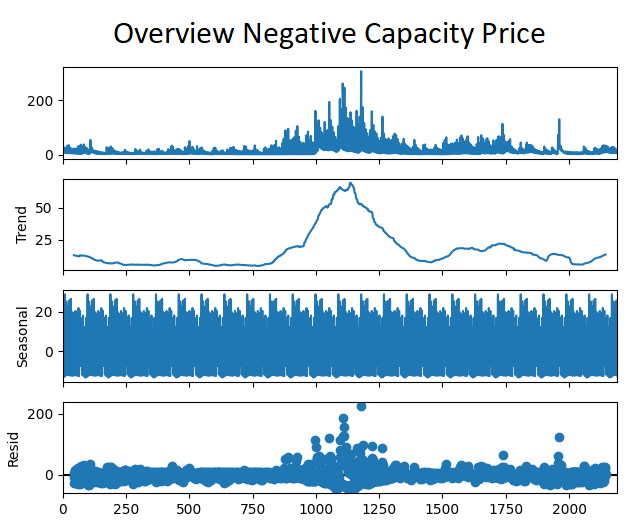
\includegraphics[width=0.7\linewidth]{pictures/capacityData_overview.png}
	\caption{Total Average Negativ Capacity Price}
	\label{fig:Overview Average Negativ Capacity Price}
\end{figure}

Bei einer genaueren Untersuchung der Saisonalität zeigt siche ein täglicher und ein leichter Wöchentlicher rythmus in den Daten.
Da es sich um Daten handelt die sich auf 4h-Blöcke beziehen sind alle 6 Lags als ein Tag zu interpretieren.
Abbildung \ref{fig:Autocorrelation Negative Capacity Price - 5 Days} zeigt dabei eine klaren täglichen rythmus in den Daten.

\todo{price in titel ergänzen}
\begin{figure}[!h]
	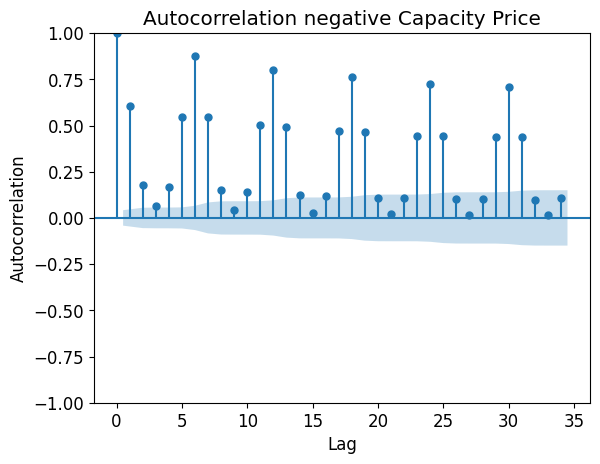
\includegraphics[width=0.7\linewidth]{pictures/Autocorrelation negative Capacity Price.png}
	\caption{Autocorrelation Negative Capacity Price - 5 Days}
	\label{fig:Autocorrelation Negative Capacity Price - 5 Days}
\end{figure}

Und Abbildung \ref{fig:AutocorrNegCap4Weeks} lässt zudem einen leichten wöchentlichen Zyklus erkennen.
\begin{figure}[!h]
	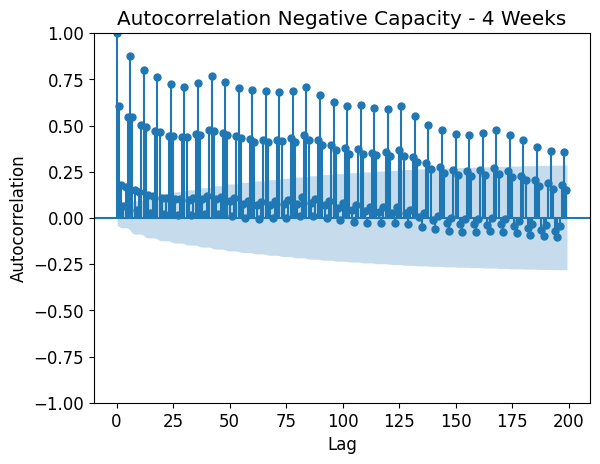
\includegraphics[width=0.7\linewidth]{pictures/Autocorrelation Negative Capacity - 4 Weeks.png}
	\caption{Autocorrelation Negative Capacity Price - 4 Weeks}
	\label{fig:AutocorrNegCap4Weeks}
\end{figure}

Die Preise zu den positiven Kapazitätwerten verhalten sich ähnlich wie die negativen Kapazitätswerte.

Zur anaylse und Zeitreihenvorhersage dieser Daten bieten sich nun, aufgrund der starken autocorrelation verschiedene statistische methoden an.
Dabei stellt sich besonders die ARIMA methode heraus. Diese beruht auf autoregression und ist somit besonders gut für zeitreihen mit starker
autorkorrelation geeignet. Um auch die Saisonalen effekte gut abbilden zu können gibt es eine Variante the ARIMA methode die SARIMA methode.

Ein ausführlicher Test der SARIMA methode, und der dafür notwendigen Tests befindet sich in Appendix \todo{verweis einfügen}. Dabei hat sich gezeigt, das die SARIMA methode schwächen mit der
komplexität in sehr langen Zeitreihen hat. So stieg die Rechenzeit expotential an und langfriste vorhersagen zeigten eine klare verzerrung hinsichtlich des letzten Trends.
Da wir aber kurzfristig ähnliche Jahresverläufe erwarten ist diese verzerrung folgend dem Trend am Jahresende nicht sinnvoll.
Außerdem ist die SARIMA analyse dafür ausgelegt Zeitreihendaten mit nur einer saisonalität zu erstellen. Für multiple Saisonalitäten wären aufwendige
manuelle anpassungen nötig. Ein Algorithmus der diese Nachteile vermeidet fußt auf den vorher genannten Konzepten und nennt sich TBATS.
TBATS is acronym for Trigonometric seasonality Box-Cox transformation ARMA errors Trend Seasonal components. Dieser Algorithmus von SKTIME erlaubt eine
einfachere Zeitreihenvorhersage bei gegebener multipler Saisonalität \cite{.05.04.2025}. \todo{appendix verweis}

Die somit vorhergsagte Zeitreihe ähnelt sehr der realen Zeitreihe [Abbildung \ref{fig:Negative Capacity Price Prediction - 2023}]. zu Beachten ist das die hier zu sehende Zeitreihe die Zeitreihe mit der höchsten Wahrscheinlichkeit ist.
So liegen 50\% der möglichen betrachteten Werte darüber und 50\% darunter. Wenn wir mit hilfe des vortrainierten predictors mehrere Szenarien/Zeitreihen
erstellen wollen so führt die inherente steigende ungewissheit mit steigenden Zeitabstand zu einer größerem intervall in dem die Daten liegen [Abbildung \ref{fig:Negative Capacity Price Prediction Interval - 2023}].
Das macht inhaltlich sinn und mag für viele anwendungsfälle sinnvoll sein, wir gehen aber davon aus das die mittlere vorhersage nicht an genauigkeit verliert
und wollen daraus szenarien generieren. Zu diesem Zweck wird die wahrscheinlichste/mittlere zeitreihenvorhersage genommen und manuel nach oben und nach unten
um bestimmte Prozentsäte hoch bzw. herunterskaliert. Die so erstellten Preisvorhersagen werden dann mit den realen Preisen verglichen und berechnet zu wievielen
Prozent mit der skalierten Zeitreihe ein Gebotszuschlag erfolgt wäre.

\begin{figure}[!h]
	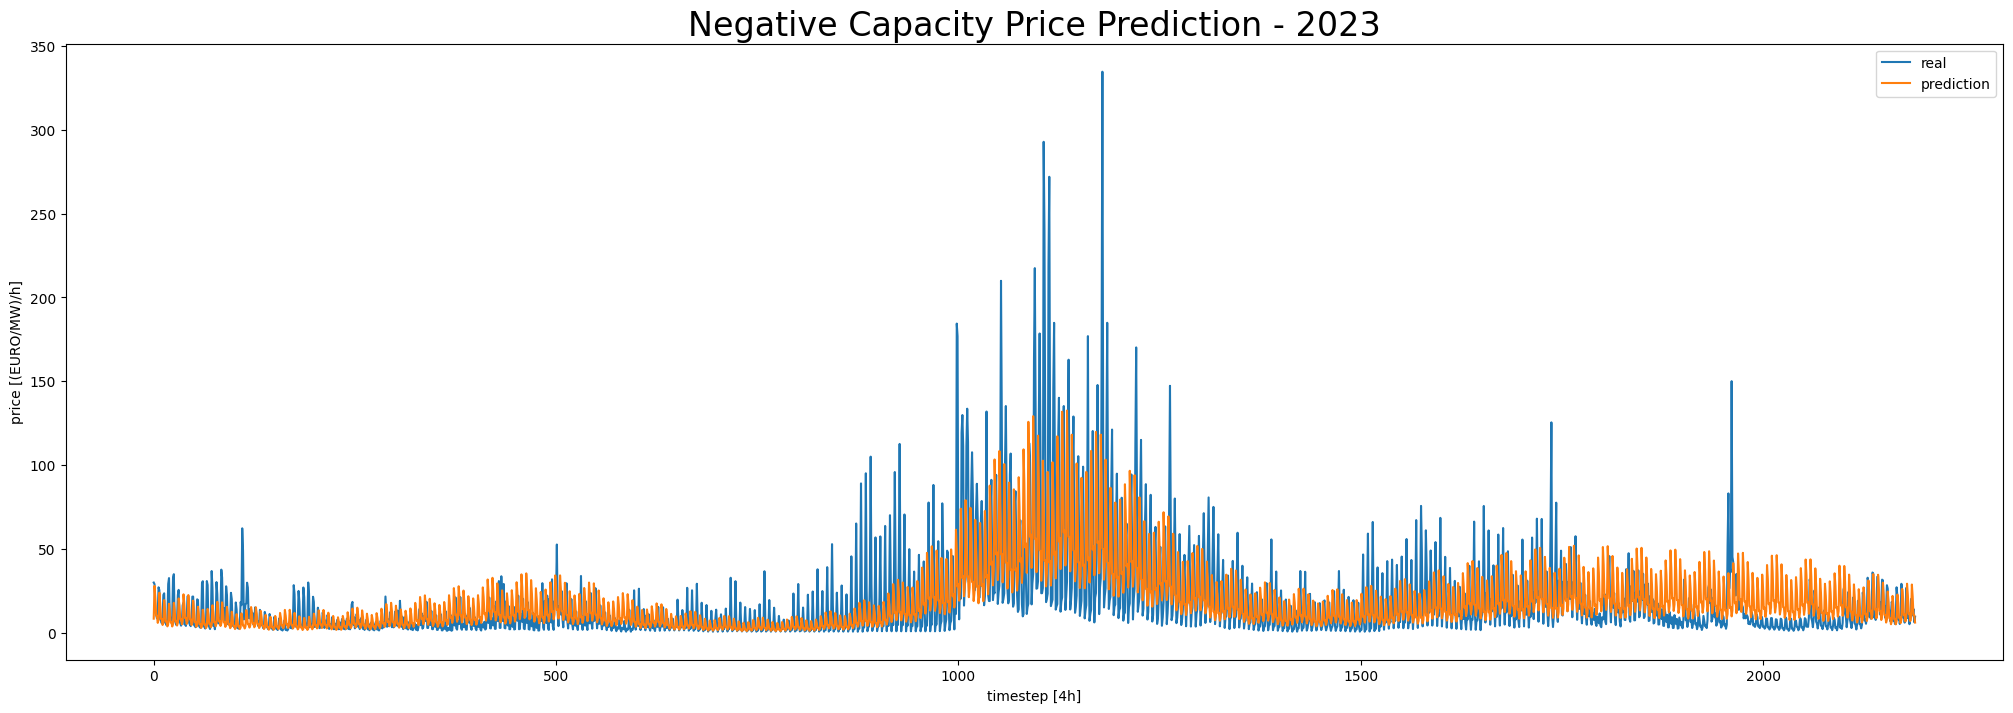
\includegraphics[width=1\linewidth]{pictures/RL/Negative Capacity Price Prediction - 2023.png}
	\caption{Negative Capacity Price Prediction - 2023}
	\label{fig:Negative Capacity Price Prediction - 2023}
\end{figure}

\begin{figure}[H]
	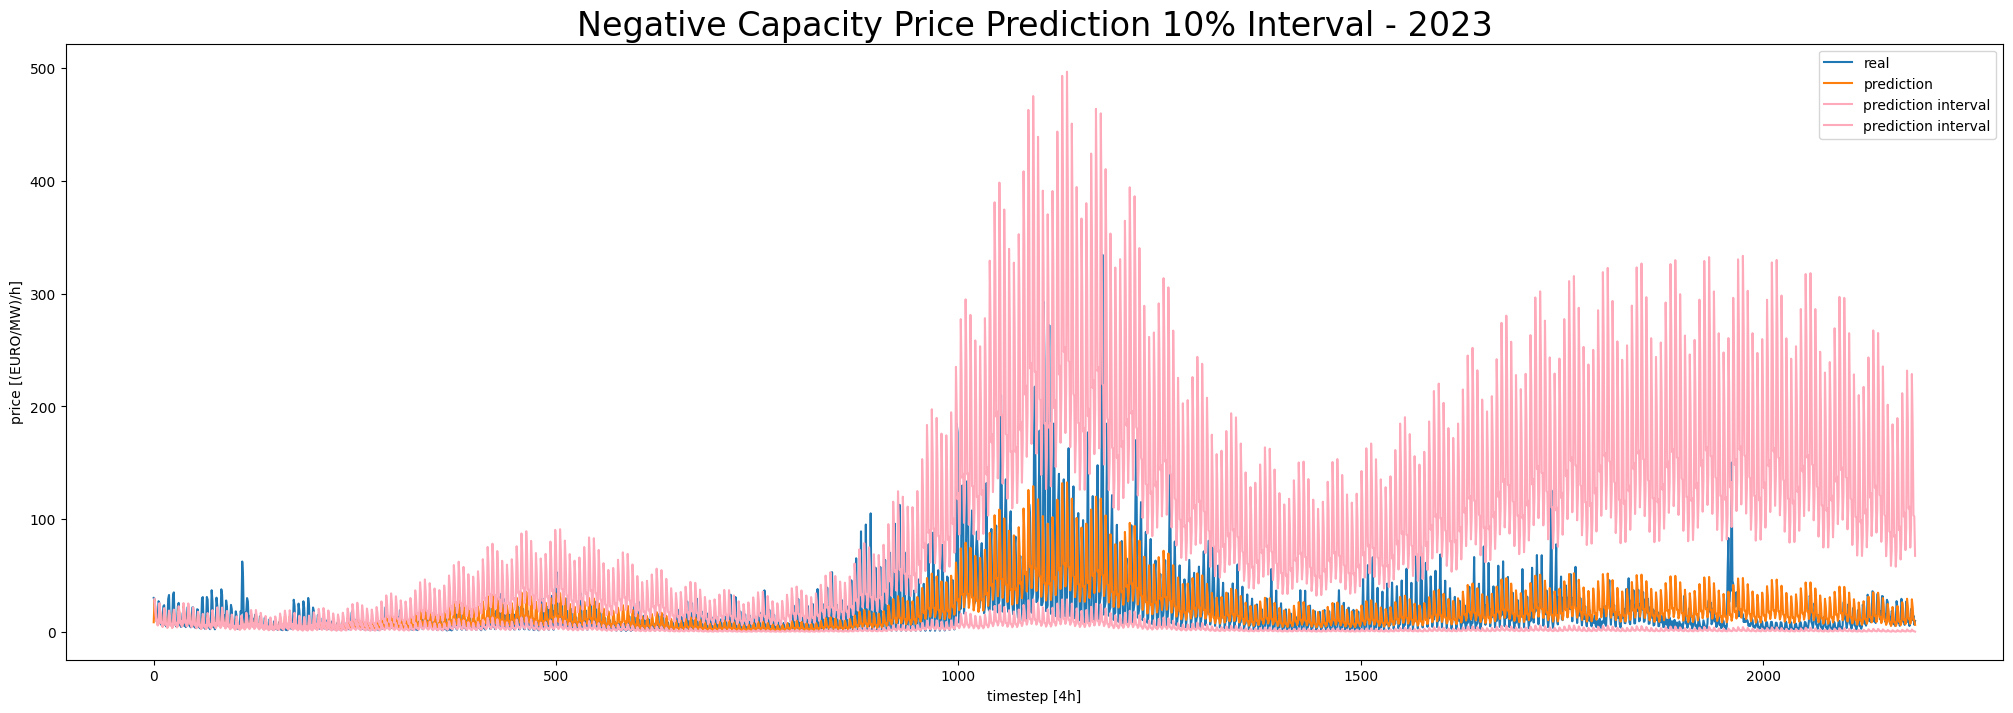
\includegraphics[width=1\linewidth]{pictures/RL/Negative Capacity Price Prediction Interval - 2023.png}
	\caption{Negative Capacity Price Prediction 10\% Interval - 2023}
	\label{fig:Negative Capacity Price Prediction Interval - 2023}
\end{figure}

- hier eventuell noch rein das wenige daten ein hohes rauschen erzeugen
- wobei zuviele daten ein overfitting verursachen können



\textbf{DA}\\
Die Day-Ahead Markt Preise sind zwar Variabel unterliegen aber einem Täglichem wie Wöchentlichen Rythmus.
Im Jahresverlauf sind nur allgemeine Trends ablesbar wie Abbildung \ref{fig:overviewDAprices} zeigt.
\begin{figure}[!h]
	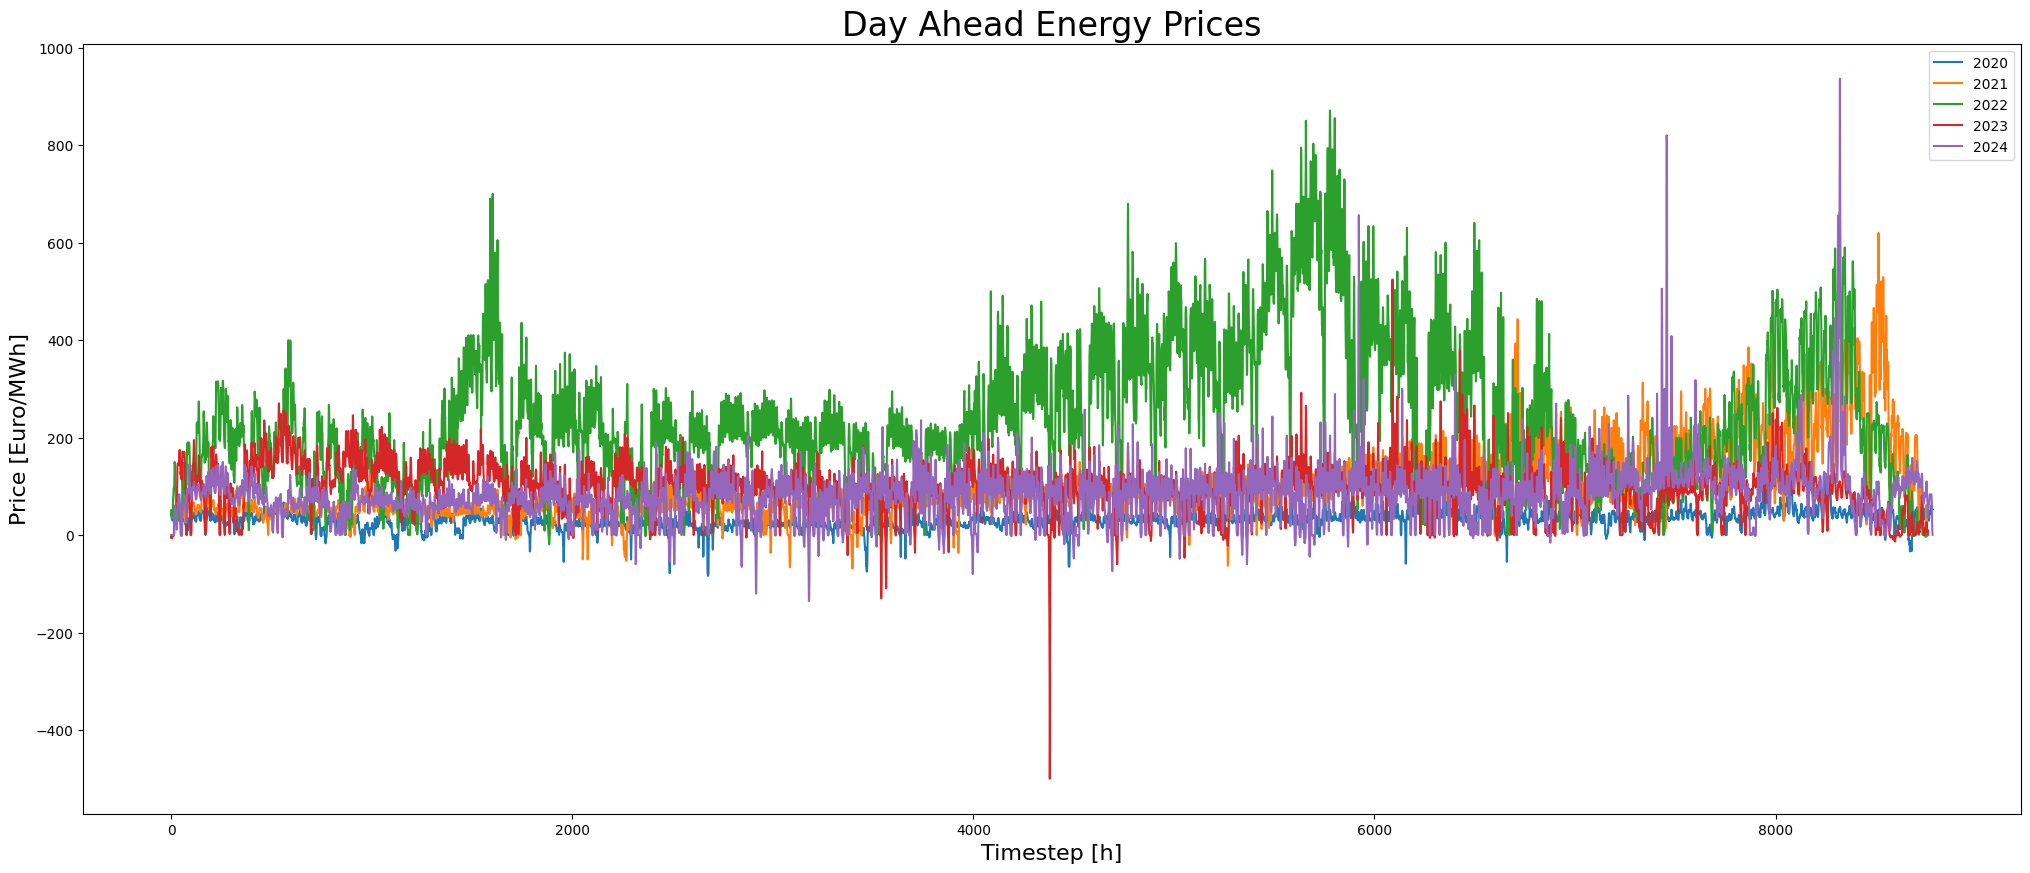
\includegraphics[width=1\linewidth]{pictures/overviewDAprices_year.png}
	\caption{Overview DA prices}
	\label{fig:overviewDAprices}
\end{figure}
Die außergewöhnliche Kurvenbewegung im Jahr 2022 ist mit dem Angriffskrieg Russlands gegen die Ukraine zu erklären
und den daraus folgenden Turbulenzen am Gas Markt.

Da es sich beim DA Markt um einen pay-as-cleared markt handelt (alle bekommen den Preis des am höchsten bezugschlagtem Teilnehmers)
und wir als Produzent erneurbarer Energien mit sehr geringen Opperationalen Kosten zu tun haben ist es für das model nur wichtig ob
wir am markt teilnehmen und welcher clearing price zu erwarten ist.

wie and Grafik \ref{fig:meanDA2020} bis \ref{fig:stdDA2024}      zu entnehmen ist zeigt der clearing price einen täglichen und wöchentlich  rythmus.
Das Nivau verändert sich zwar lässt sich aber gut verhersagen. Aufgrund des Marktdesigns brauchen wir auch nur einen erwarteten clearing price
da wir in der Realität ein 0-Preis Gebot abgeben können und somit sogut wie sicher bezuschlagt werden.
Der Erwartete Preis wird für unser Model als Mittelwert der Jahre 2020 bis 2024 ohne das Jahr 2022 kalkuliert. So erhalten die
Saisonale Struktur in den Daten und gleichen Ausreißer nach oben sowie nach unten aus. So ergibt sich je nach Tageszeit, Wochentag und Jahresverlauf ein zuverlässig
zu erwartender clearing-price. Das Nivau kann auch noch nachträglich leicht durch einen Skalierungsfaktor angepasst werden ohne die inherente Struktur der Daten zu gefährden.

\begin{figure}[H]
	\centering
	\begin{minipage}{0.49\textwidth}
		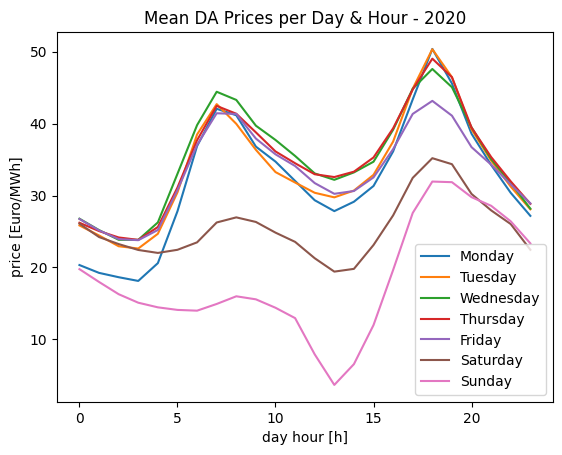
\includegraphics[width=1\linewidth]{pictures/DA/Mean DA Prices per Day and Hour - 2020.png}
		\subcaption{Mean DA-Price}
		\label{fig:meanDA2020}
	\end{minipage} \hfill
	\begin{minipage}{0.49\textwidth}
		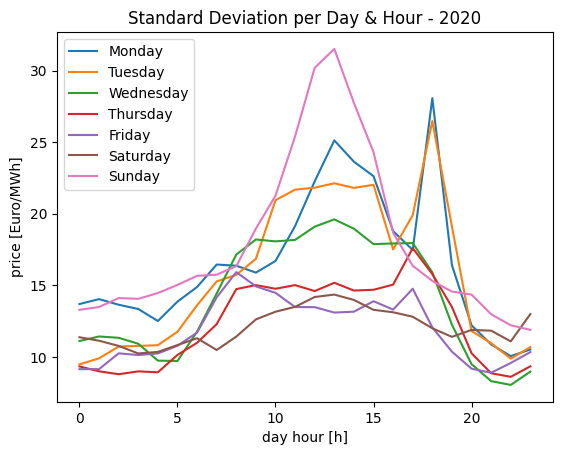
\includegraphics[width=1\linewidth]{pictures/DA/Standard Deviation per Day and Hour - 2020.png}
		\subcaption{Standard Deviation DA-Price}
		\label{fig:stdDA2020}
	\end{minipage}
	\caption{Daily and hourly DA-Data - 2020 }
\end{figure}

\begin{figure}[H]
	\centering
	\begin{minipage}{0.49\textwidth}
		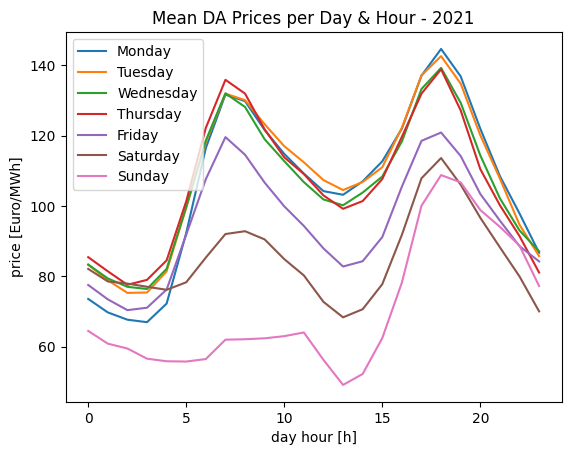
\includegraphics[width=1\linewidth]{pictures/DA/Mean DA Prices per Day and Hour - 2021.png}
		\subcaption{Mean DA-Price }
		\label{fig:meanDA2021}
	\end{minipage} \hfill
	\begin{minipage}{0.49\textwidth}
		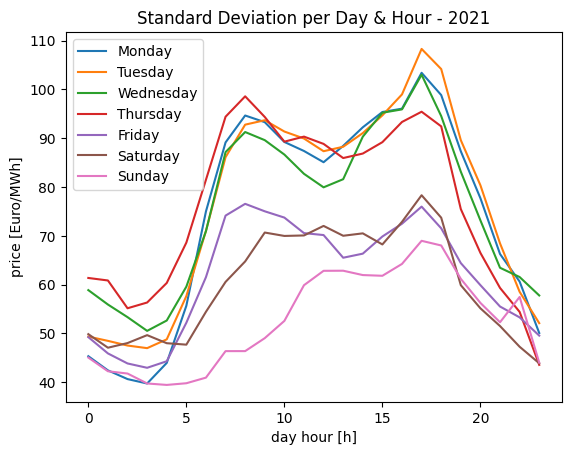
\includegraphics[width=1\linewidth]{pictures/DA/Standard Deviation per Day and Hour - 2021.png}
		\subcaption{Standard Deviation DA-Price}
		\label{fig:stdDA2021}
	\end{minipage}
	\caption{Daily and hourly DA-Data - 2021 }
\end{figure}

\begin{figure}[H]
	\centering
	\begin{minipage}{0.49\textwidth}
		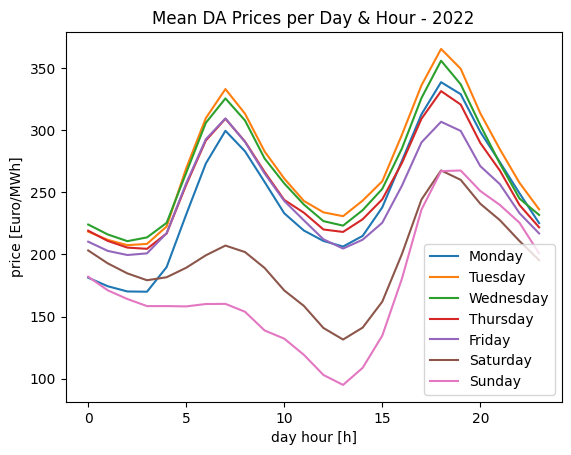
\includegraphics[width=1\linewidth]{pictures/DA/Mean DA Prices per Day and Hour - 2022.png}
		\subcaption{Mean DA-Price }
		\label{fig:meanDA2022}
	\end{minipage} \hfill
	\begin{minipage}{0.49\textwidth}
		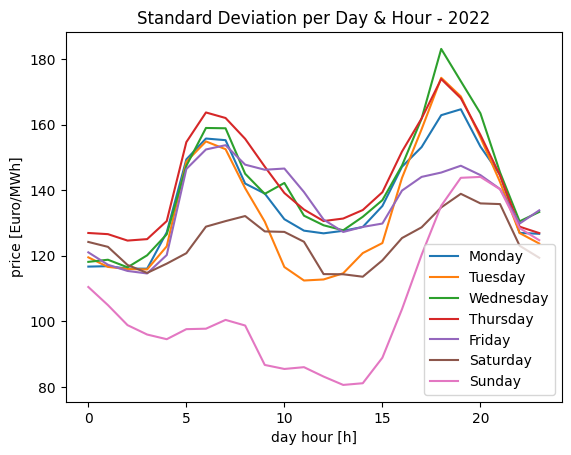
\includegraphics[width=1\linewidth]{pictures/DA/Standard Deviation per Day and Hour - 2022.png}
		\subcaption{Standard Deviation DA-Price}
		\label{fig:stdDA2022}
	\end{minipage}
	\caption{Daily and hourly DA-Data - 2022 }
\end{figure}

\begin{figure}[H]
	\centering
	\begin{minipage}{0.49\textwidth}
		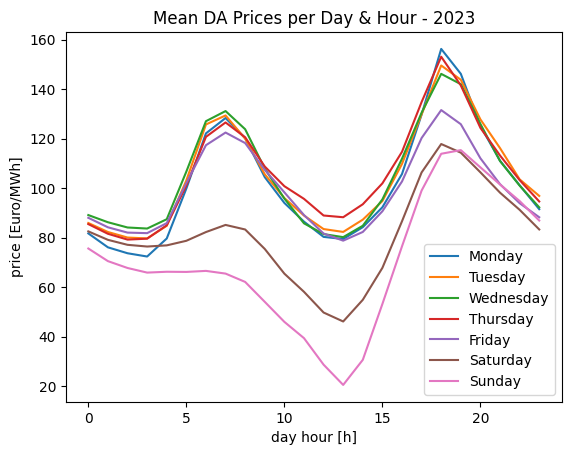
\includegraphics[width=1\linewidth]{pictures/DA/Mean DA Prices per Day and Hour - 2023.png}
		\subcaption{Mean DA-Price }
		\label{fig:meanDA2023}
	\end{minipage} \hfill
	\begin{minipage}{0.49\textwidth}
		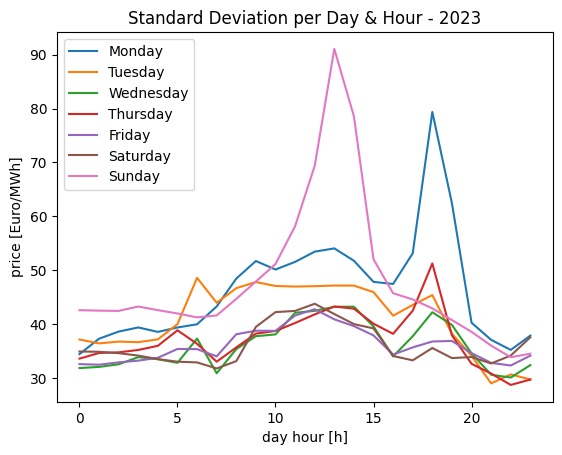
\includegraphics[width=1\linewidth]{pictures/DA/Standard Deviation per Day and Hour - 2023.png}
		\subcaption{Standard Deviation DA-Price}
		\label{fig:stdDA2023}
	\end{minipage}
	\caption{Daily and hourly DA-Data - 2023 }
\end{figure}

\begin{figure}[H]
	\centering
	\begin{minipage}{0.49\textwidth}
		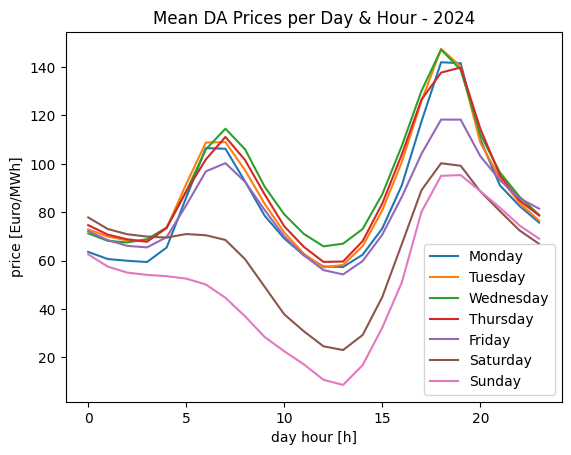
\includegraphics[width=1\linewidth]{pictures/DA/Mean DA Prices per Day and Hour - 2024.png}
		\subcaption{Mean DA-Price }
		\label{fig:meanDA2024}
	\end{minipage} \hfill
	\begin{minipage}{0.49\textwidth}
		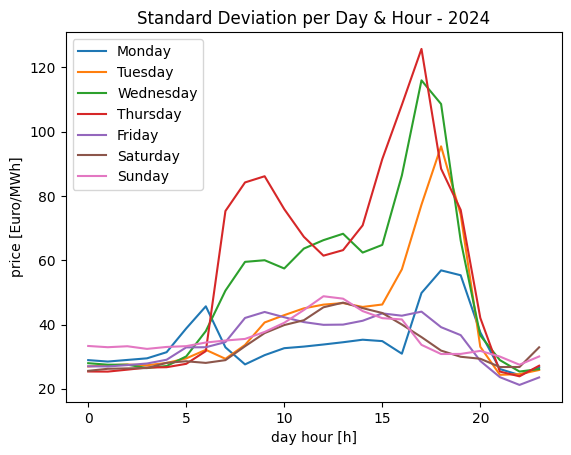
\includegraphics[width=1\linewidth]{pictures/DA/Standard Deviation per Day and Hour - 2024.png}
		\subcaption{Standard Deviation DA-Price}
		\label{fig:stdDA2024}
	\end{minipage}
	\caption{Daily and hourly DA-Data - 2024 }
\end{figure}
\todo{ziel für das hoch und runter setzten der linie ... -> erklärung was ich damit bezwecken möchte in dem entsprechendem Mark .. habe ich das schon mit drinne?}


\textbf{RA}\\
Die RA unterliegen einer sehr hohen Variabilität und lassen sich nur sehr schwer statistisch vorherzusagen. So
verfügen sie nur über eine sehr schwache autocorrelation mit nur ganz leichtem wöchentlichem rythmus \ref{fig:Autocorrelation Positive Energy Price}.

hier ist der angebotspreis nicht zwar nicht für den profit ausschlaggebend aber für die abbrufwahrscheinlichkeit
die dann wiederum zur modellierung unserer Batteriespeichstatuses wichtig ist.
\begin{figure}[!h]
	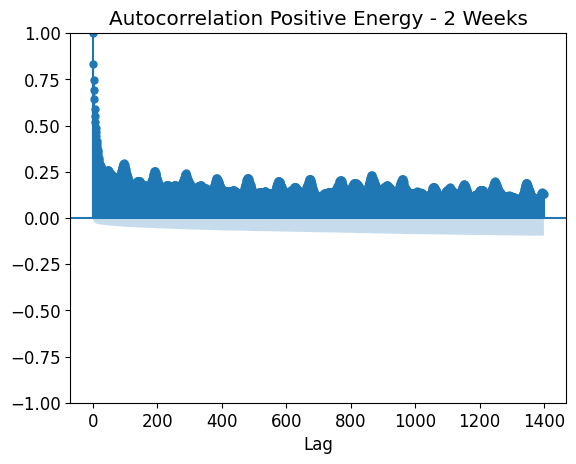
\includegraphics[width=1\linewidth]{pictures/Autocorrelation Positive Energy - 2 Weeks.png}
	\caption{Total Average Positive Energy Price}
	\label{fig:Autocorrelation Positive Energy Price}
\end{figure}

Auch Trends sind in den Daten keine vorhanden. So zeigt die Abbildung \ref{fig:posEngOverview} beispielhaft jeweils 30 Tage aus dem frühen, mittleren und spätem Jahresverlauf.
Auch hier sind weder Trends noch Saisonale entwicklungen zu erkennen.

\begin{figure}[!h]
	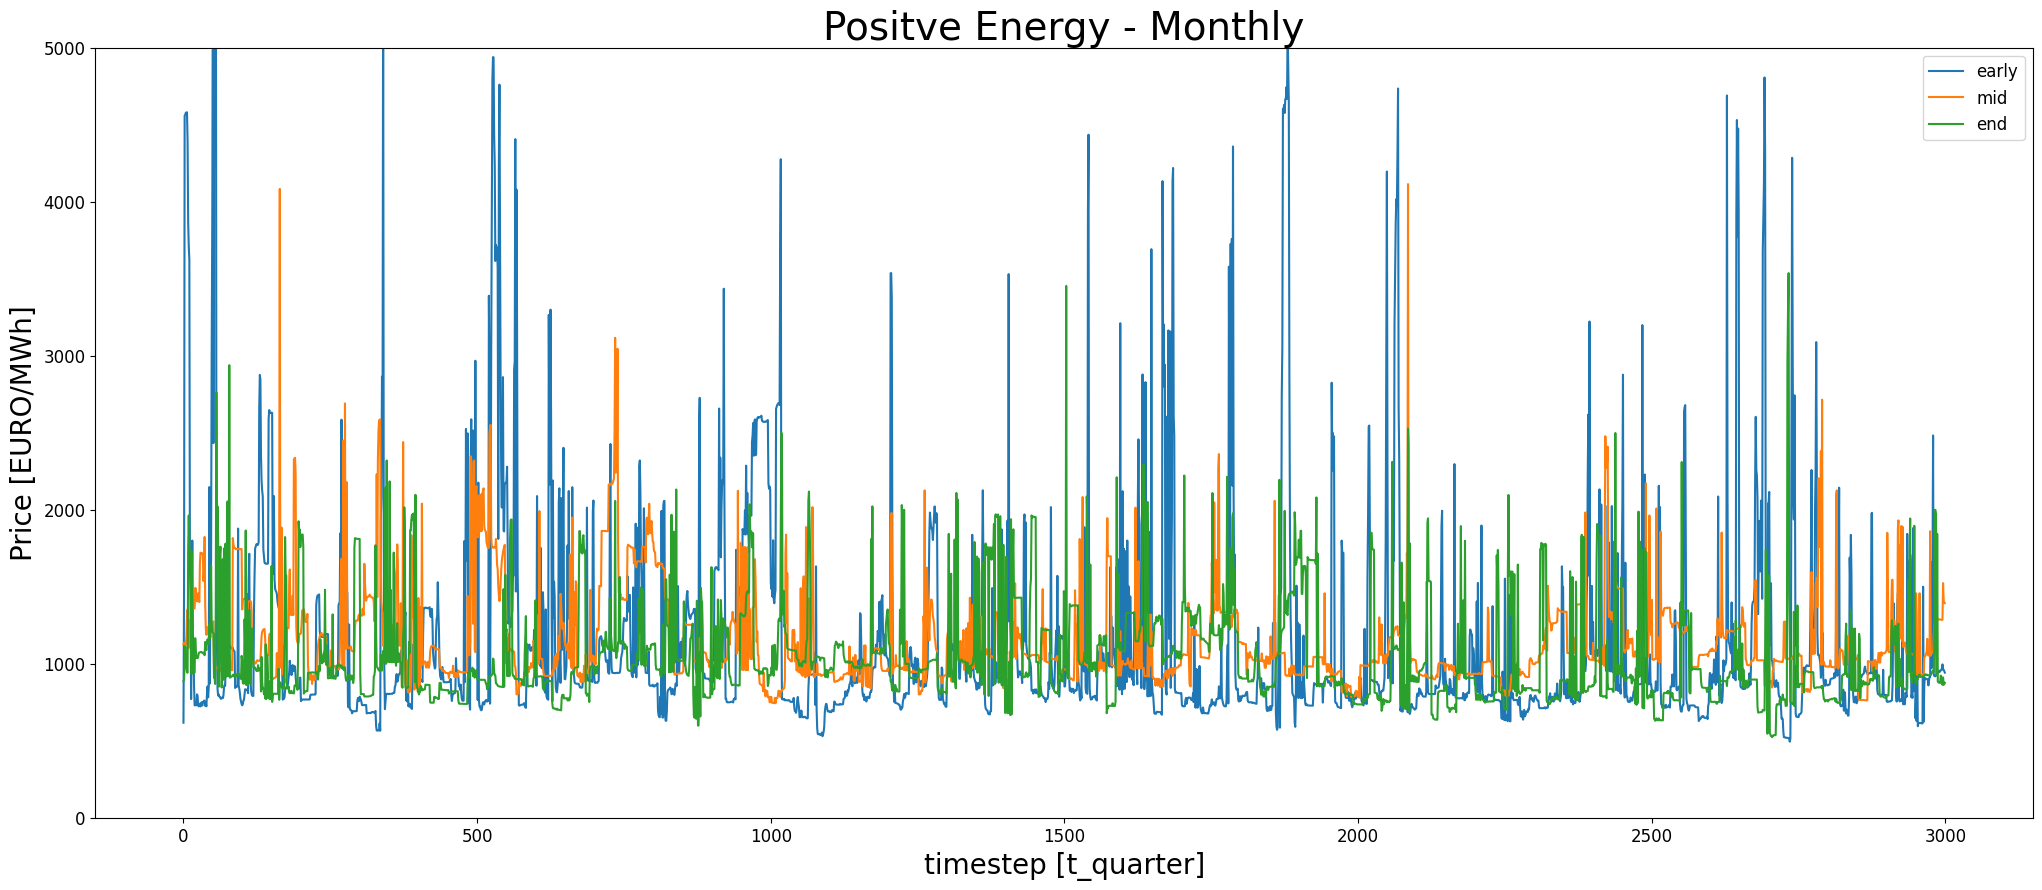
\includegraphics[width=1\linewidth]{pictures/posEngOverview.png}
	\caption{Overview Positive Energy Price}
	\label{fig:posEngOverview}
\end{figure}
\todo{das ist eine grafik mit den alten average preise, mache eine graifk mit den richtigen grenzpreisen}
\todo{grafiken verschiedene Preisszenarien}
\todo{appendix verweis zu python code}

Zu szenario generation werden Realmarkt daten aus dem Jahre 2023 herangezogen.
Das Jahr 2023 wird zuerst hinsichtlich volatiler Energiequellen untersucht [siehe Tabelle \ref{tab:energy_sources_std}].
Hierbei zeigt sich das besonders Solar und Wind Onshore Kraftwerke einer volatilen Produktion unterliegen.

\begin{table}[ht]
	\centering
	\begin{tabular}{|l|r|}
		\hline
		\textbf{Source}                 & \textbf{Standard Deviation} \\
		\hline
		Geothermal                      & 5.956190                    \\
		Fossil Oil                      & 85.360298                   \\
		Waste                           & 133.320136                  \\
		Hydro Water Reservoir           & 167.126363                  \\
		Hydro Run-of-river and poundage & 310.405850                  \\
		Biomass                         & 429.594441                  \\
		Nuclear                         & 1223.169733                 \\
		Hydro Pumped Storage            & 1543.402759                 \\
		Wind Offshore                   & 1833.588012                 \\
		Fossil Gas                      & 2916.794393                 \\
		Fossil Hard coal                & 3364.505964                 \\
		Fossil Brown coal/Lignite       & 3799.694920                 \\
		\textbf{Solar}                  & \textbf{9879.907341}        \\
		\textbf{Wind Onshore}           & \textbf{10506.831136}       \\
		\hline
	\end{tabular}
	\caption{Standard deviation per energy generator type}
	\label{tab:energy_sources_std}
\end{table}

Anschließend wird die summierte Produktion von Solar und Wind Onshore je Zeitpunkt berchnet und
durch die gesamte Produktion aller Kraftwerke zum gleichen Zeitpunkt geteilt. So erzielen wir den relativen
Anteil dieser besonders volatilen Kraftwerke an der gesamten Produktion. Die These ist nun das wenn ein Vorhersagefehler eintritt
dieser besonders starke Auswirkungen hat, da er einen größeren Anteil an der Gesamtproduktion betrifft.
Diese relativen Produktionsdaten volatiler Kraftwerke werden nun in 36 Quantile eingeteilt. Das erste, mittlere und letzten
Quantil werden nun zur Szenariogeneration benutzt.

Hierfür werden die Zeitpunkte der Quantile, die auf stündlichen Daten beruhen, auf einen viertelstündlichen rythmus extrapoliert und
dazugehörigen Regelarbeitsmarkt daten vom betreffenden Zeitabschnit exportiert.

So ergeben sich 10 mögliche Szenarien für Tage mit hoher, mittlerer und niedrigem Anteil einer volatilem Produktion. Die wahrscheinlichkeit
wird dabei als gleichverteilt angenommen, so das jedes Szenario die eine Wahrscheinlichkeit von 10\% hat.

Abbildung   bis
\todo{abbildungen ergänzen}
zeigt nun das zwar das allgemeine Preisniveau steigt, aber da man mit dem hohen Anteil erneuerbarer Energien
kalkuliert und somit auf die hohe volatilität eingeplant ist halten sich ansonsten die Auswirkugen in grenzen.
Die sehr hohen Ausreißer scheinen sich in den Szenarien zu zeigen in denen man nicht mit all zu hohen außreißern rechnet.
\todo{den teil drinne lassen?}



Data from ENTSOE transperency platform
\todo{ref entsoe}
-->appendix
\todo{Python Code appendix verweis}


%--> kann über  mondpreis eskapen\\
%--> können eine kaum genutzte szenarioeplosion vermeiden (wording nochmal überarbeiten)\\
%- vereinfachung der RL markt mechanik/restriktionen
%--> stellen über batterie gleichung sicher das wir immer liefer können und vermeiden so komplexe $q_RA$ restriktionen (wann wie wo gelten)\\
%--> wir stellen einfach sicher das wir immer liefern könnten und fertig\\


- verschiedene Methoden ...
-> implementiert in python
-> alle können dem model hinzugefügt werden
-> ich habe dann aus diesen und jenen gründe diese Variante gewählt

\section{Simplification}

wir betrachten uns als teil eines bieterbundes
Um den rechenaufwand und die komplexität des models zu begrenzen wurden ein paar vereinfachungen vorgenommen.
Diese vereinfachungen beschränken kaum die realitätsnähe des Models.

Nochfolgende eine geordnete Aufführung welche Vereinfachungen getroffen wurden.
\subsubsection{RL}
\subsubsection{DA}
\subsubsection{RA}
\subsubsection{Battery Storage Status}






\chapter{Results}

Um die Ergebnisse richtig einordnen zu können stellen wir an dieser stelle kurz die Ausgangsdaten dar.

Die relativen Produktionsquantile die zum exportieren der anderen Zeitreihenabschnitte gedient haben stellen sich wie folgt dar:

\begin{figure}[!h]
	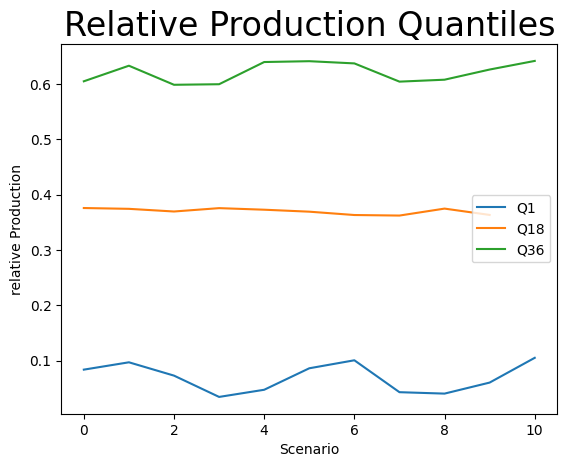
\includegraphics[width=0.7\linewidth]{pictures/results/relativeProduktionQuantils.png}
	\caption{Relative Production Quantiles}
	\label{fig:Relative Production Quantiles}
\end{figure}

Die daraus Resultierenden Zeitreihen für aktivierte Regelarbeit und deren Preise stellen sich dann wie folgt dar:

Für den selben Zeitabschnitt lässt sich der DA Markt wie folgt zusammenfassen:


Außerdem stellt sich der entsprechende RL Markt wie folgt dar:

Dabei zeigt sich das mit steigender Marktdurchdringung der volatilen Energieproduktionsquellen vor allem die Menge an aktivierter Negativer
RegelArbeit steigt während die nachfrage nach positiver regelarbeit fällt.

Ein ähnliches Bild zeigt sich bei den Grenzpreisen für die aktivierte Regelarbeit. wärend die Preise für negative Regelarbeit mit
zunehmenden Anteil an volatilen Produzenten zunimmt, gehen die Preise für die positive Regelarbeit zurück.

Bemerkenswert ist allerdings das sehr hohe Ausreißer in den Zeitreihen für die Grenzpreise der  positiven Regelarbeit bei mittlere und geringer
Marktdurchdringung durch volatile Produzenten zu sehen ist.
--> das liegt vermutlich daran das in den Szenarien wo man mögliche große schwankungen erwartet darauf vorbeiretet ist.
--> Aber in den Szenarien in denen die mehrheit der Anbieter nicht damit rechnet scheint eine unerwartet hohe Nachfrage
--> einen preisschock aus zu lösen.

Die medianen \todo{eventuell nochmal erklärung in data abschnitt wieso das hier die medianen sind} KApazitätspreise für Regelarbeit peaken
sowohl für die negative als auch für die positive im mittleren Szenario. In den Daten des ersten Quantils sind die sie für die negative Regelleistung
vergleichbar mit denen des 36. Quantils. Für die positive Regelleistung hebt sich das 36. Quantil von 1. Quantil vor allem im späten Tagesverlauf ab.

--> es scheint so als würden viele anbieter damit rechnen am folgenden Tag Regelarbeit zu liefern. Dabei hantiert der Regelleistungspreis
--> als eine Art mitnahme preis was zur folge hat das das Angebot noch stärker steigt als die Nachfrage und so sinkende Regelleistungspreise zur folge hat.

Auf Grundlage dieser Zeitreihen hat das Model folgende Daten ermittelt.

Die Strategie für die Gebotspreise für den Kapazitätsmarkt bewegt sich über alle Szenarien hinweg knapp unterhalb des erwarteten Grenzpreises.
\todo{grafik hierfür einblenden  .. !! eher wichtig !!}

Zu sehen ist das die Bereitstellung der negativen RegelArbeit
in den niedrigen und mittleren Szenarien früher erfolgt wenn beide Regelleistungsgebot angenommen wurden [Figure \ref{fig:Negative Balance Energy - Q1}, \ref{fig:Negative Balance Energy - Q18}].
--> verpflichtungen und insgesamt regelmäßigere ladekurve wärend in den höheren Preisszenarien mehr wert
--> darauf gelegt wird wirklich die preisspitzen möglichst optimal mit nehmen zu können.
--> ob das in der realität oder perfektes wissen innerhalb des szenarios so erfolgen kann ist fraglich
In den Szenarien mit den hoher produktiver volatilität ist diese Verschiebung nicht fest zu stellen [Figure \ref{fig:Negative Balance Energy - Q36}]


Wärend sich die Gebotsmengen zur postiven Regelarbeit, je nach Bezuschlagung am Regelleistungsmarkt,
kaum in dem niedrigen und mittleren Szenario voneinander unterscheiden. sind deutlichere Unterschiede
im Szenario mit hoher volatiler Produktion zu erkennen. Auch hier erfolgt eine frühere Bereitstellung
der Arbeit bei stärkeren Restriktionen durch die Bezugschlagung am Regelleistungsmarkt.



Zum Verständnis
\begin{enumerate}
	\item Restricted: B $\rightarrow$ accepted RL in \& out
	\item Restricted: O $\rightarrow$ accepted RL out \& declined in
	\item Restricted: I $\rightarrow$ accepted RL in \& declined out
	\item Restricted: N $\rightarrow$ declined RL in \& out
\end{enumerate}

Die Ergebnisse zeigen eine relativ stetiges Gebotsverhalten am Kapazitätsmarkt über alle Szenarien hinweg.

-->Es wird gerade soviel Geboten
das der Batteriespeicher immer sicher die Restriktionen erfüllen kann ohne all zu sehr den Regelarbeitsmarkt zu beeinflussen.

\begin{figure}[!h]
	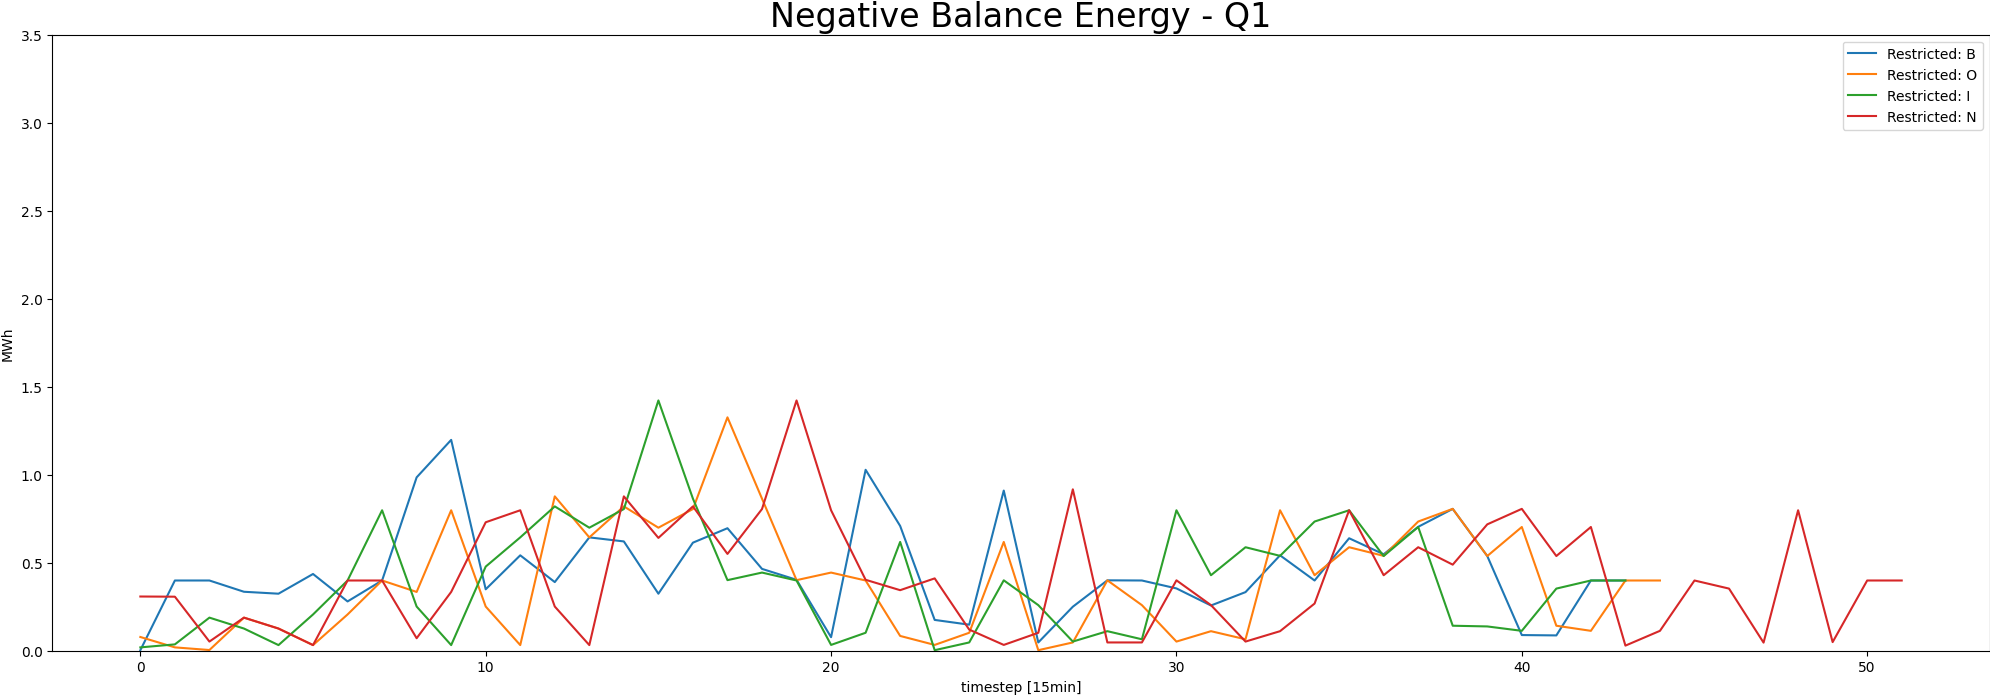
\includegraphics[width=1\linewidth]{pictures/results/Negative Balance Energy - Q1.png}
	\caption{Negative Balance Energy - Q1}
	\label{fig:Negative Balance Energy - Q1}
\end{figure}

\begin{figure}[!h]
	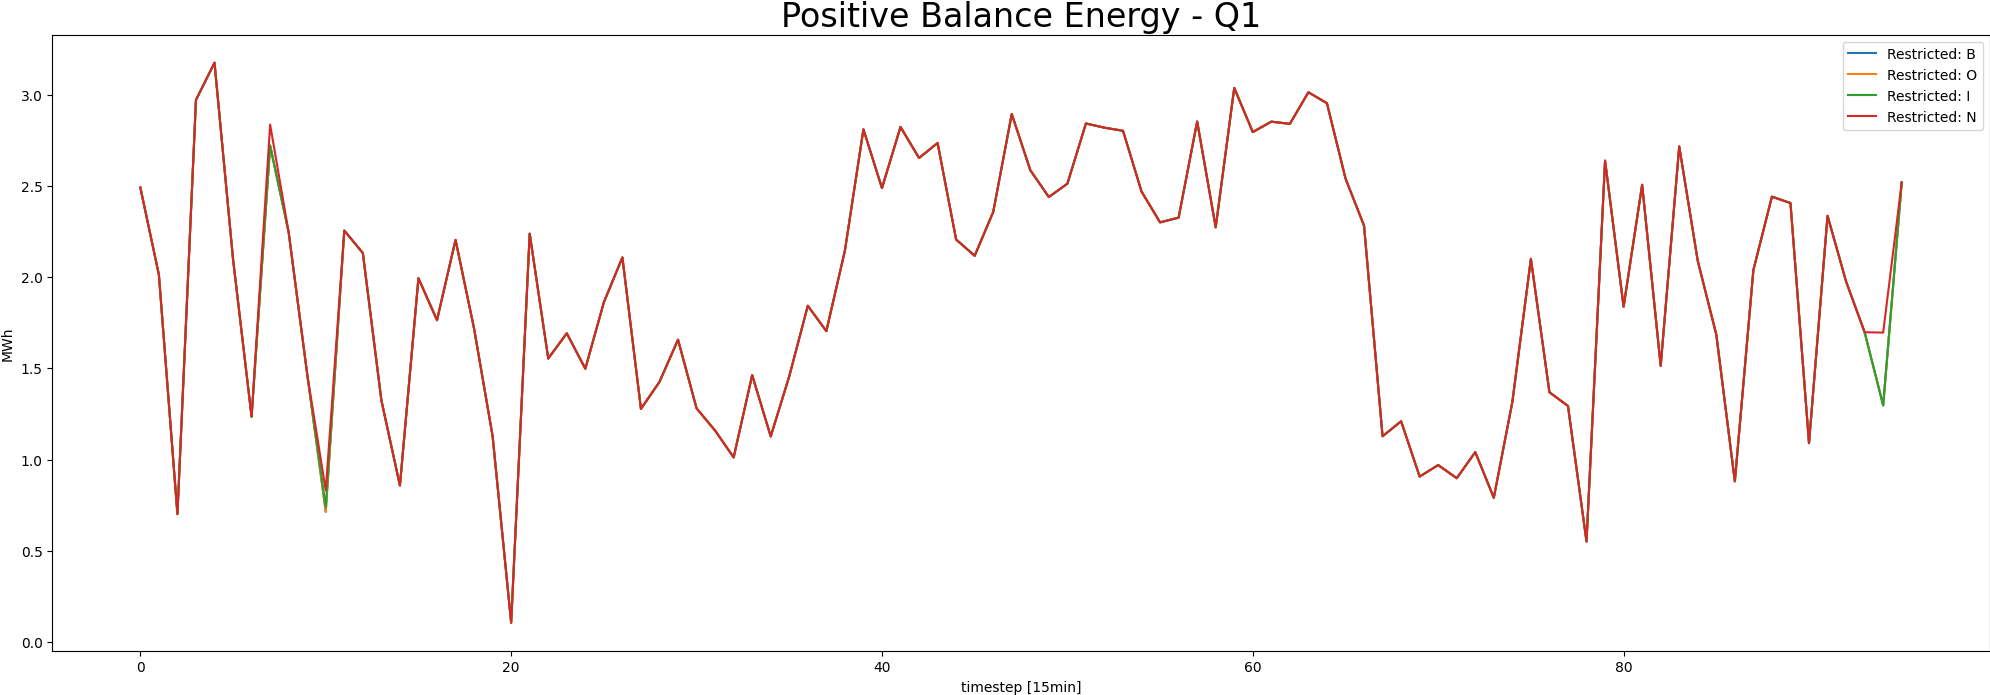
\includegraphics[width=1\linewidth]{pictures/results/Positive Balance Energy - Q1.png}
	\caption{Negative Balance Energy - Q1}
	\label{fig:Negative Balance Energy - Q1}
\end{figure}



\begin{figure}[!h]
	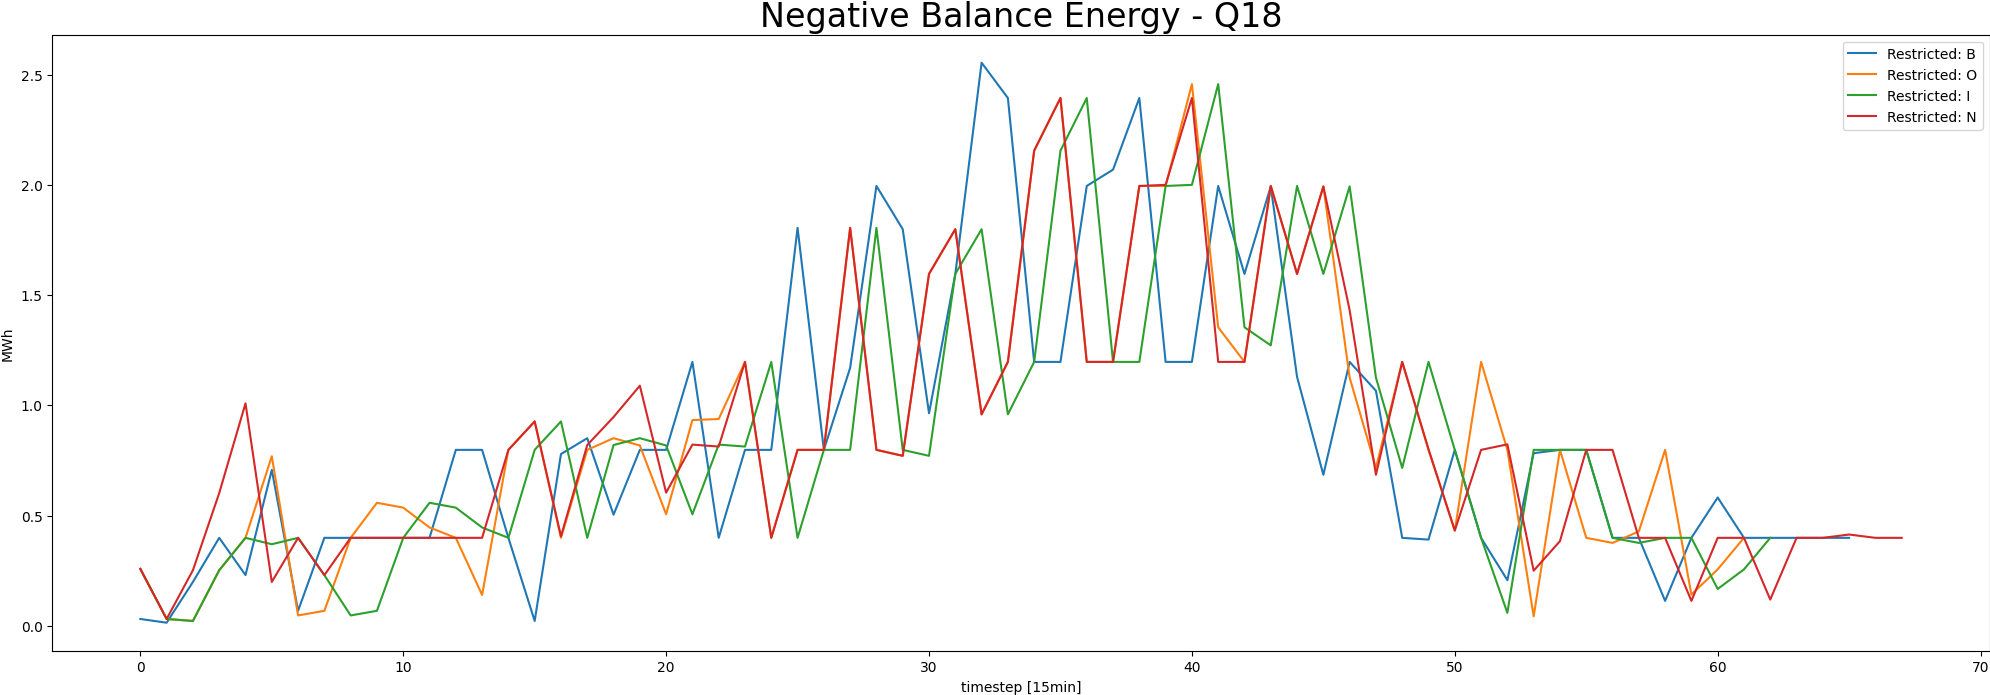
\includegraphics[width=1\linewidth]{pictures/results/Negative Balance Energy - Q18.png}
	\caption{Negative Balance Energy - Q18}
	\label{fig:Negative Balance Energy - Q18}
\end{figure}

\begin{figure}[!h]
	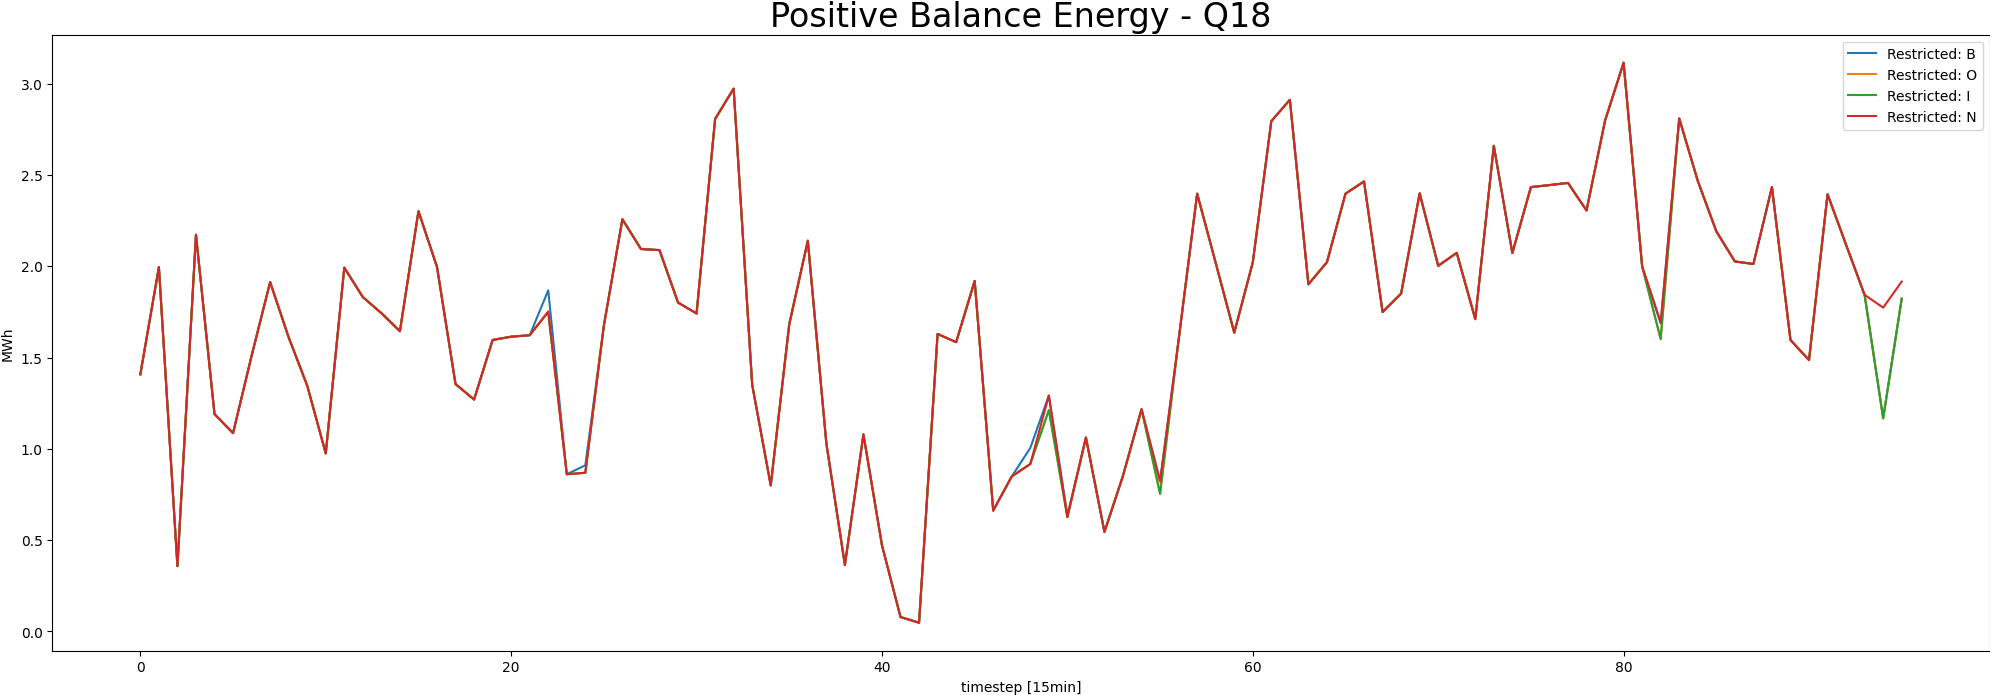
\includegraphics[width=1\linewidth]{pictures/results/Positive Balance Energy - Q18.png}
	\caption{Negative Balance Energy - Q18}
	\label{fig:Negative Balance Energy - Q18}
\end{figure}




\begin{figure}[!h]
	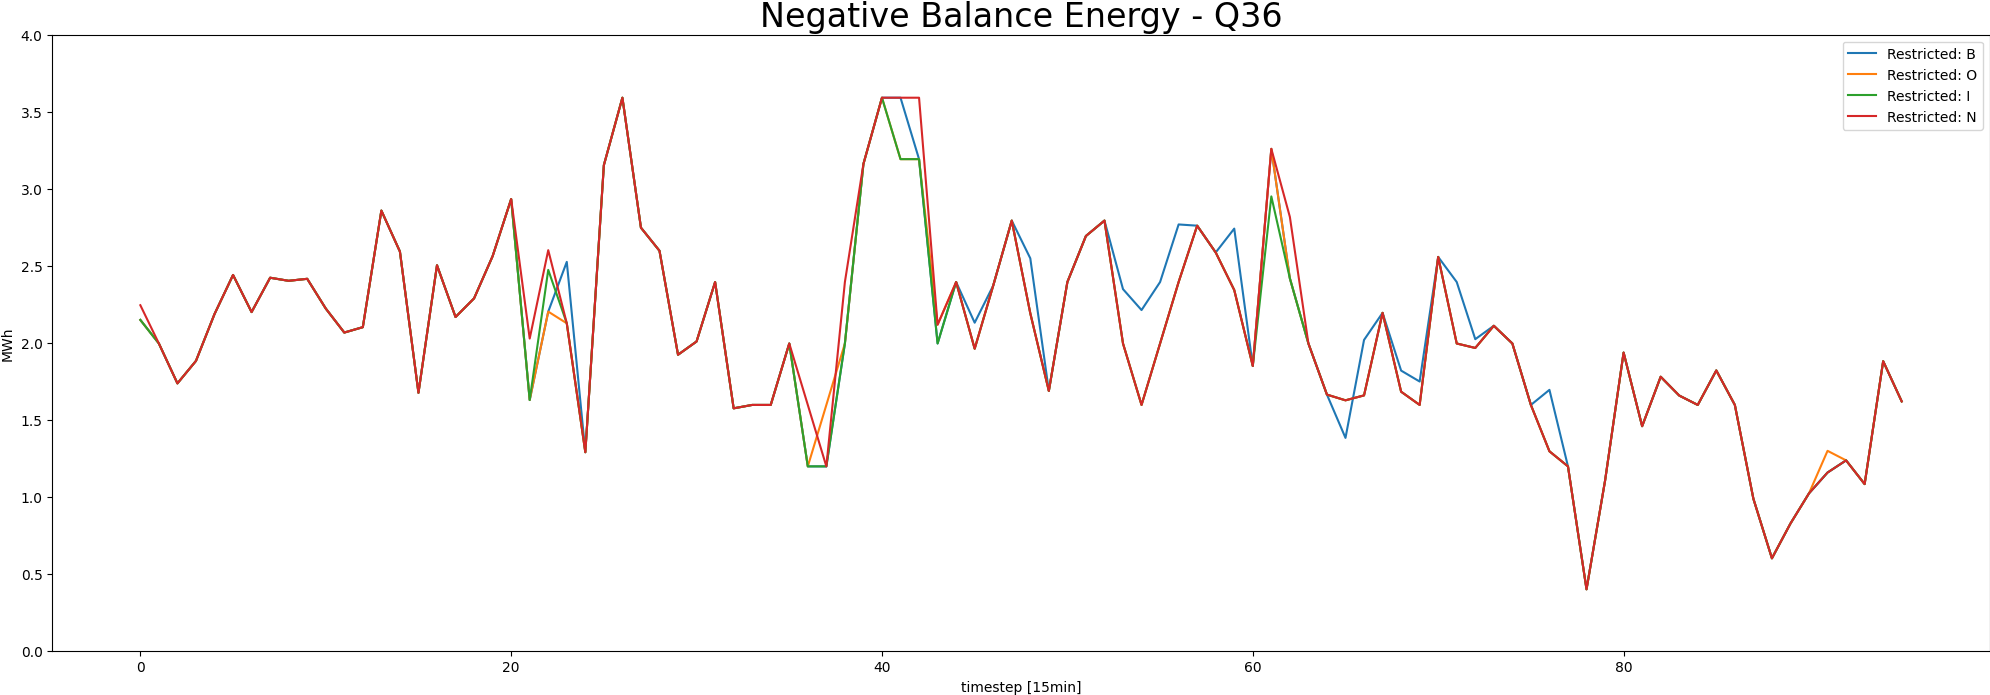
\includegraphics[width=1\linewidth]{pictures/results/Negative Balance Energy - Q36.png}
	\caption{Negative Balance Energy - Q36}
	\label{fig:Negative Balance Energy - Q36}
\end{figure}

\begin{figure}[!h]
	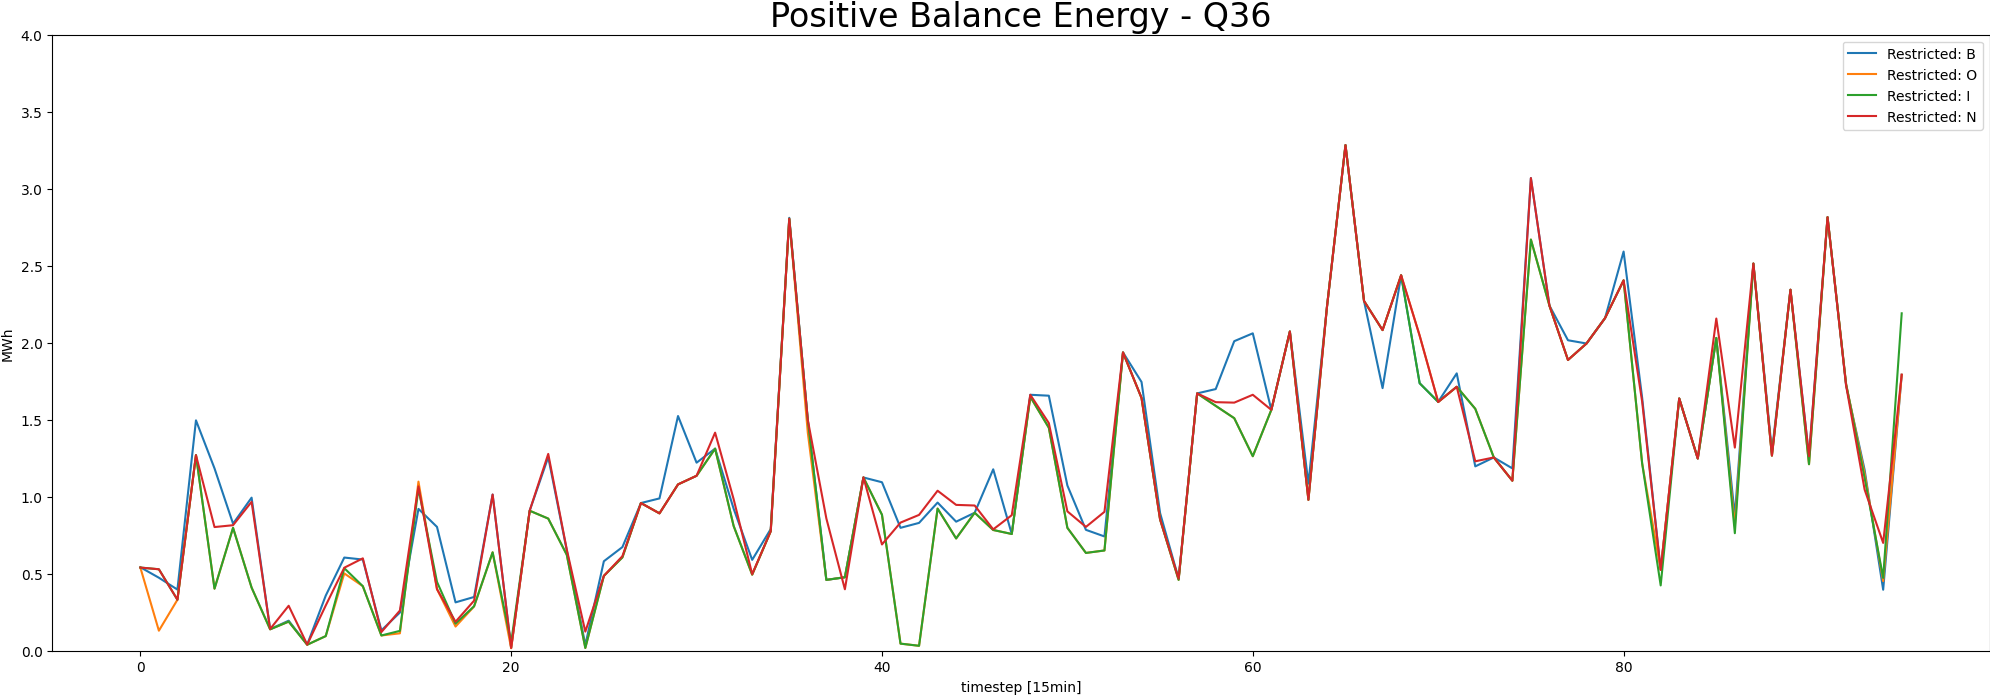
\includegraphics[width=1\linewidth]{pictures/results/Positive Balance Energy - Q36.png}
	\caption{Negative Balance Energy - Q36}
	\label{fig:Negative Balance Energy - Q36}
\end{figure}



\chapter{Conclusion}

Die vorliegenden Analysen zeigen deutlich, dass eine zunehmende Marktdurchdringung durch volatile Energieerzeuger
signifikante Auswirkungen auf die Inanspruchnahme sowie die Preisbildung von Regelarbeit hat.
Insbesondere ist zu beobachten, dass mit steigendem Anteil volatiler Erzeugung die Menge aktivierter negativer Regelarbeit zunimmt,
während gleichzeitig die Nachfrage nach positiver Regelarbeit zurückgeht. Dieses Muster spiegelt sich auch in den Grenzpreisen wider:
Während die Preise für negative Regelarbeit in Abhängigkeit zur Volatilität der Erzeugung steigen, sinken die Preise für positive
Regelarbeit tendenziell.

Auffällig sind zudem starke Preisausreißer bei der positiven Regelarbeit in Szenarien mit geringer oder mittlerer Marktdurchdringung
durch volatile Erzeuger. Diese scheinen auf unerwartet hohe Nachfragespitzen zurückzuführen zu sein, welche in Szenarien auftreten,
in denen Marktteilnehmer nicht mit großen Schwankungen gerechnet haben. Daraus lässt sich schließen, dass die Erwartungshaltung und
Vorbereitung der Marktakteure auf volatile Einspeisung entscheidend zur Preisstabilität beiträgt.

Die analysierten Kapazitätspreise zeigen ein differenziertes Bild: Die Medianwerte peaken sowohl für positive als auch negative
Regelarbeit im mittleren Szenario. Dies deutet auf eine erhöhte Wettbewerbsintensität in diesen Szenarien hin. Gleichzeitig
lässt sich aus den unteren Quantilen ableiten, dass bei negativer Regelarbeit selbst im Vergleich von Q1 zu Q36 kaum Unterschiede
bestehen, während bei positiver Regelarbeit gegen Tagesende eine stärkere Preisdivergenz sichtbar wird. Daraus kann geschlossen werden,
dass Anbieter in Szenarien mit erwarteter hoher volatilät für den Folgetag mit einer Regelarbeitsbereitstellung rechnen und dabei den Kapazitätspreise
als opportunistischen  „Mitnahmepreis“ gestalten. Dies führt dazu, dass das Angebot in Relation zur Nachfrage überproportional
steigt und folglich sinkende Arbeitspreise resultieren.

Die Gebotsstrategien für den Regelleistungsmarkt bewegen sich über alle Szenarien hinweg knapp unterhalb des erwarteten Grenzpreises.

In den Szenarien mit niedriger und mittlere volatiler Producktion zeigt eine verschiebung hin zum negativen Regelleistungsmarkt. Dies zeigt sich
in einem regelmäßigeren Bereitstellung von negativer Regelarbeit. In den Szenarien mit hoher durchdringung und hohen Preisen zeigt sich
am negativen Regelarbeitsmarkt ein Trend möglichst gut die Preisspitzen mitnehmen zu können, dafür wird auf Profit am Regelleistungsmarkt
verzichtet.




Besonders im Bereich negativer Regelarbeit  ist zu erkennen, dass die Bereitstellung in Szenarien mit niedrigem und mittlerem Preisniveau
tendenziell früher erfolgt.  Dies lässt auf eine stärkere Bindung an Verpflichtungen und eine regelmäßigere Ladeplanung schließen.
In höheren Preisszenarien hingegen liegt der Fokus stärker auf einer optimalen Ausnutzung der Preisspitzen - ein Verhalten, das unter realen Marktbedingungen
nicht zwingend replizierbar ist, da es perfektes Wissen über zukünftige Preispfade voraussetzt.

Die Analyse positiver Regelarbeit verdeutlicht hingegen, dass sich Gebotsmengen in niedrig- und mittelfrequentierten Szenarien
nur geringfügig unterscheiden. Erst bei hoher Einspeisung volatiler Energien treten deutliche Unterschiede auf. Auch hier zeigt
sich: Je stärker die Restriktionen durch die Bezuschlagung im Regelleistungsmarkt, desto früher erfolgt die Bereitstellung der Regelarbeit.

Insgesamt zeigen die Ergebnisse, dass sowohl die Erwartungshaltung der Marktakteure als auch deren Strategien im Kapazitäts-
und Regelarbeitsmarkt wesentlich zur Preisbildung und zur Systemstabilität beitragen. Eine vertiefte Betrachtung
dieser Wechselwirkungen ist daher auch für regulatorische Überlegungen zur Ausgestaltung künftiger Strommärkte von zentraler Bedeutung.

\begin{enumerate}
	\item nur ein tag, eventuell kommt der richtige reload erst in zusammenhang mit mehreren tagen zum tragen
\end{enumerate}

todo{andere anbieter wirklich mit simulieren}


%% ********************
%% Backmatter
%% ********************
%\backmatter

\chapter{Appendix}
%% change chapter title to german if necessary
%% *** local page settings ***
\markright{Appendix}
\addtocontents{toc}{\protect\setcounter{tocdepth}{-1}} %decrease the depth of the appendix entry in the ToC
\setcounter{table}{0}
\setcounter{figure}{0}
\renewcommand{\thefigure}{A.\arabic{figure}}
\renewcommand{\thetable}{A.\arabic{table}}


\section{Further Model Constraints}

\begin{flalign}
	\label{parkCon_Q^{rB}_{DA}(t_{hour})}                   \sum((s_DA, s^{in}_{RL}, s^{out}_{RL}), Q^{rB}_{DA}(t_{hour}, s^{in}_{RL}, s^{out}_{RL})) \leq parkCap * parkProfile(t_{hour}) - \sum((s_DA, s^{in}_{RL}, s^{out}_{RL}), Q_rB_reload(t_{hour}, s^{in}_{RL}, s^{out}_{RL}));
\end{flalign}
\begin{flalign}
	\label{parkCon_Q^{rI}_{DA}(t_{hour})}                   \sum((s_DA, s^{in}_{RL}, s^{out}_{RL}), Q^{rI}_{DA}(t_{hour}, s^{in}_{RL}, s^{out}_{RL})) \leq parkCap * parkProfile(t_{hour}) - \sum((s_DA, s^{in}_{RL}, s^{out}_{RL}), Q_rI_reload(t_{hour}, s^{in}_{RL}, s^{out}_{RL}));
\end{flalign}
\begin{flalign}
	\label{parkCon_Q^{rO}_{DA}(t_{hour})}                   \sum((s_DA, s^{in}_{RL}, s^{out}_{RL}), Q^{rO}_{DA}(t_{hour}, s^{in}_{RL}, s^{out}_{RL})) \leq parkCap * parkProfile(t_{hour}) - \sum((s_DA, s^{in}_{RL}, s^{out}_{RL}), Q_rO_reload(t_{hour}, s^{in}_{RL}, s^{out}_{RL}));
\end{flalign}
\begin{flalign}
	\label{parkCon_Q^{rN}_{DA}(t_{hour})}                   \sum((s_DA, s^{in}_{RL}, s^{out}_{RL}), Q^{rN}_{DA}(t_{hour}, s^{in}_{RL}, s^{out}_{RL})) \leq parkCap * parkProfile(t_{hour}) - \sum((s_DA, s^{in}_{RL}, s^{out}_{RL}), Q_rN_reload(t_{hour}, s^{in}_{RL}, s^{out}_{RL}));
\end{flalign}
\section{Quantile Market Data}

\begin{figure}[!h]
	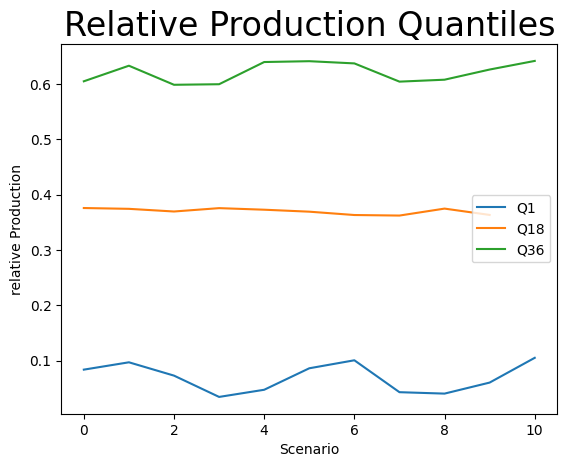
\includegraphics[width=0.7\linewidth]{pictures/results/relativeProduktionQuantils.png}
	\caption{Relative Production Quantiles}
	\label{fig:Relative Production Quantiles}
\end{figure}

Die daraus Resultierenden Zeitreihen für aktivierte Regelarbeit und deren Preise stellen sich dann wie folgt dar:
\begin{figure}[H]
	\centering

	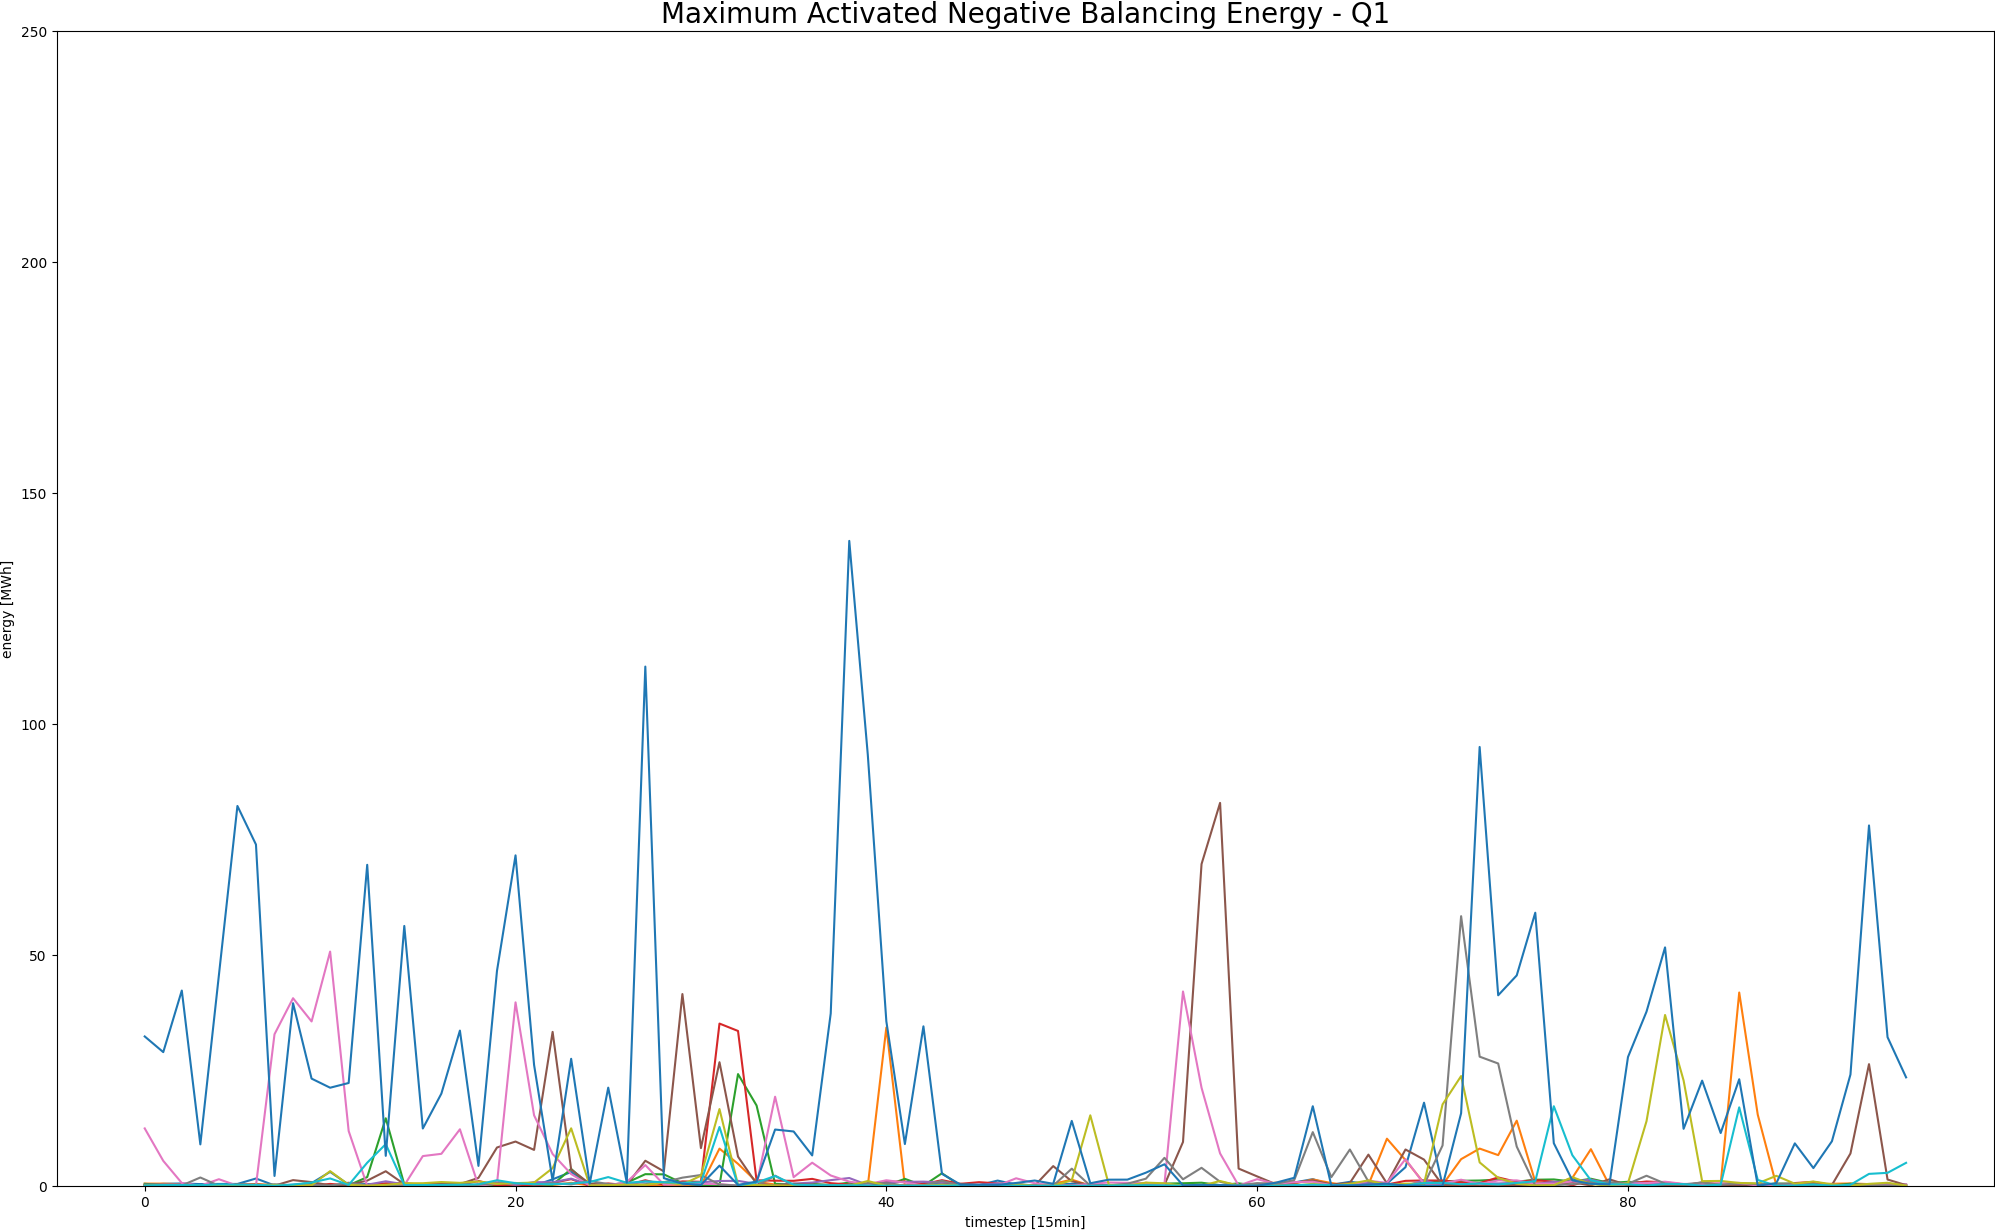
\includegraphics[width=1\linewidth]{pictures/results/Activated_negEnergy_Q1.png}
	\caption{Activated Negative Energy Q1}
	\label{fig:_negEnergy_Q1}
\end{figure}


\begin{figure}[H]
	\centering
	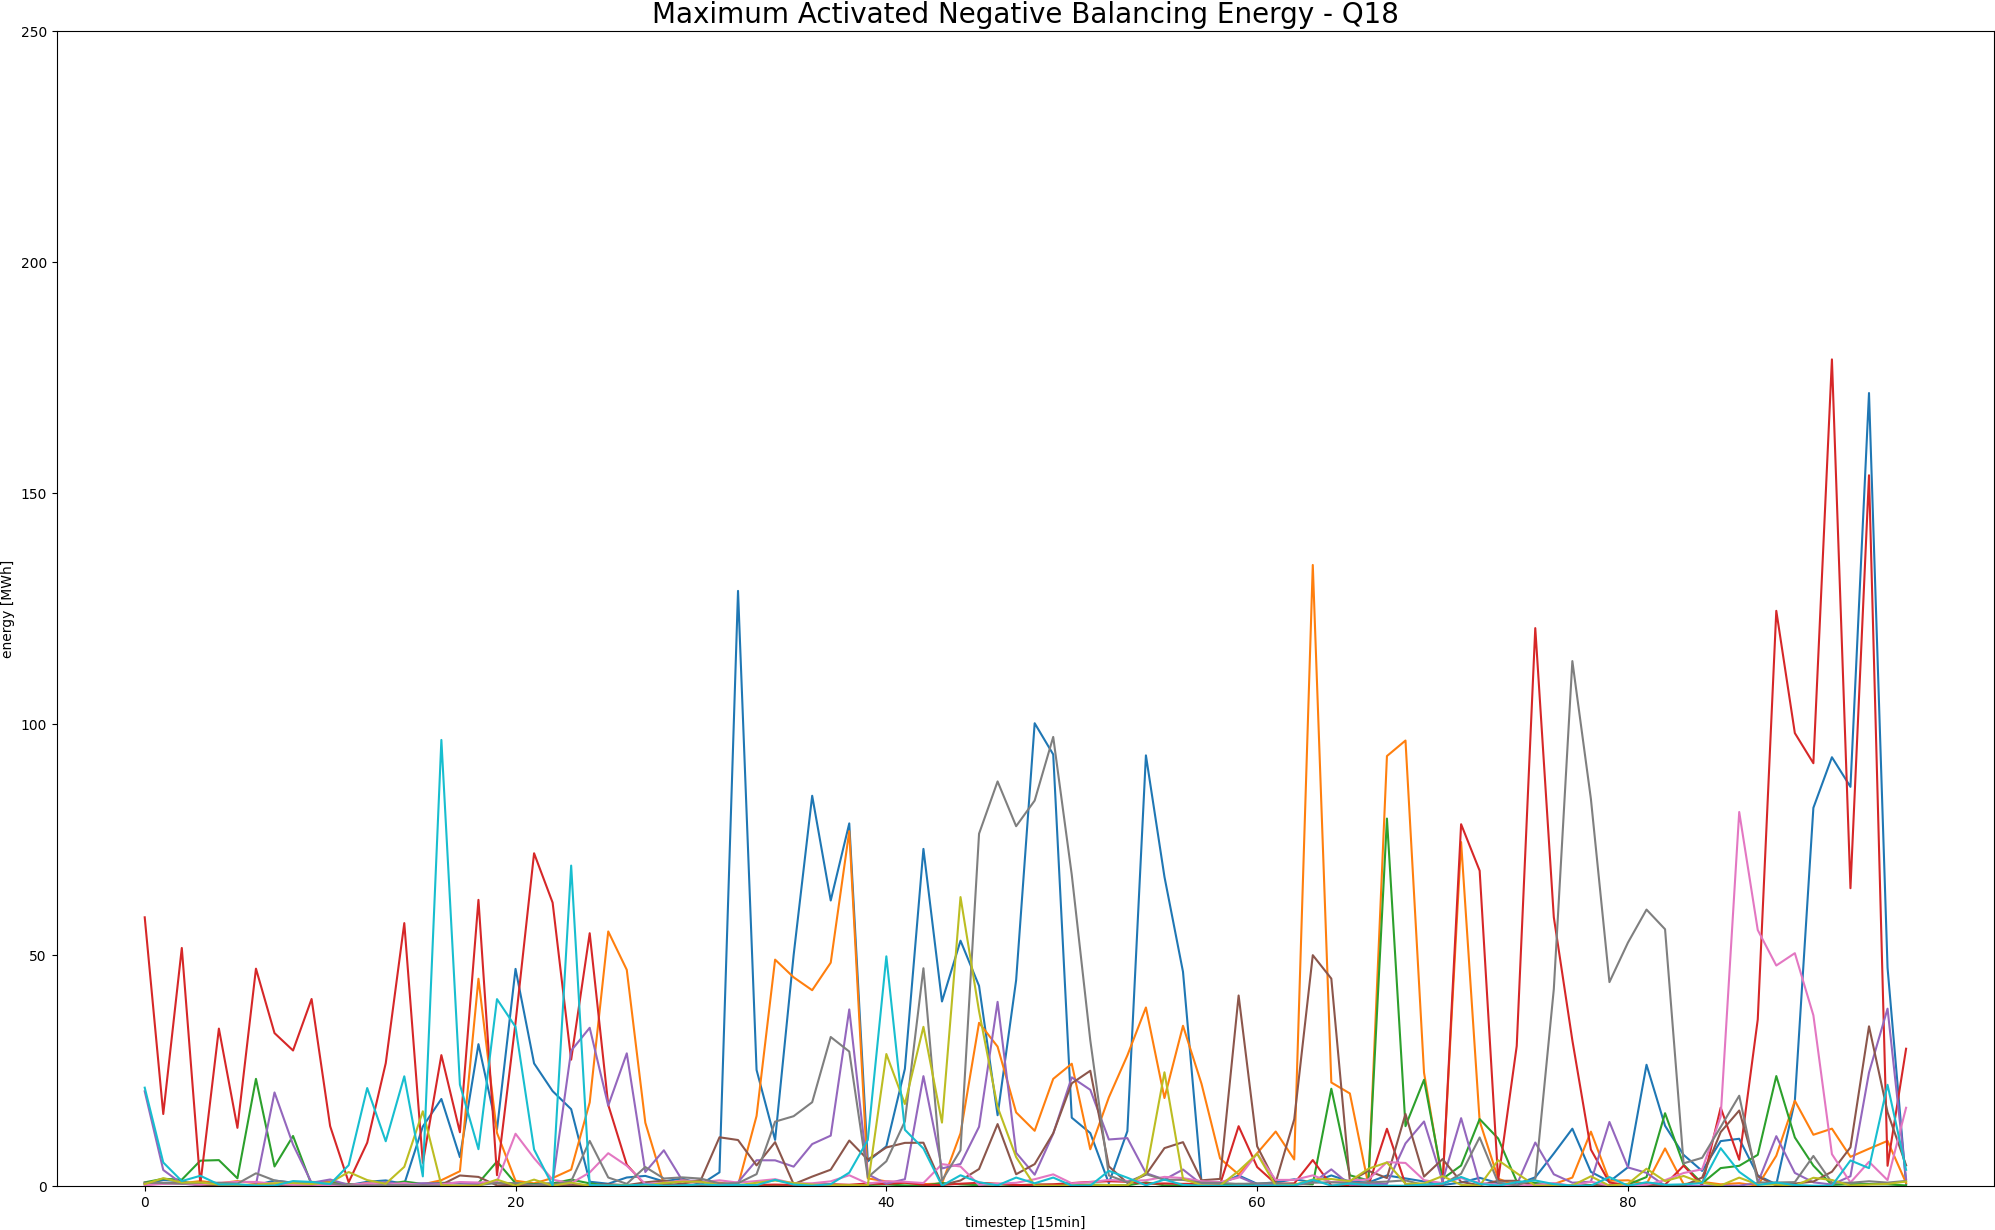
\includegraphics[width=1\linewidth]{pictures/results/Activated_negEnergy_Q18.png}
	\caption{Activated Negative Energy Q18}
	\label{fig:_negEnergy_Q18}
\end{figure}

\begin{figure}[H]
	\centering
	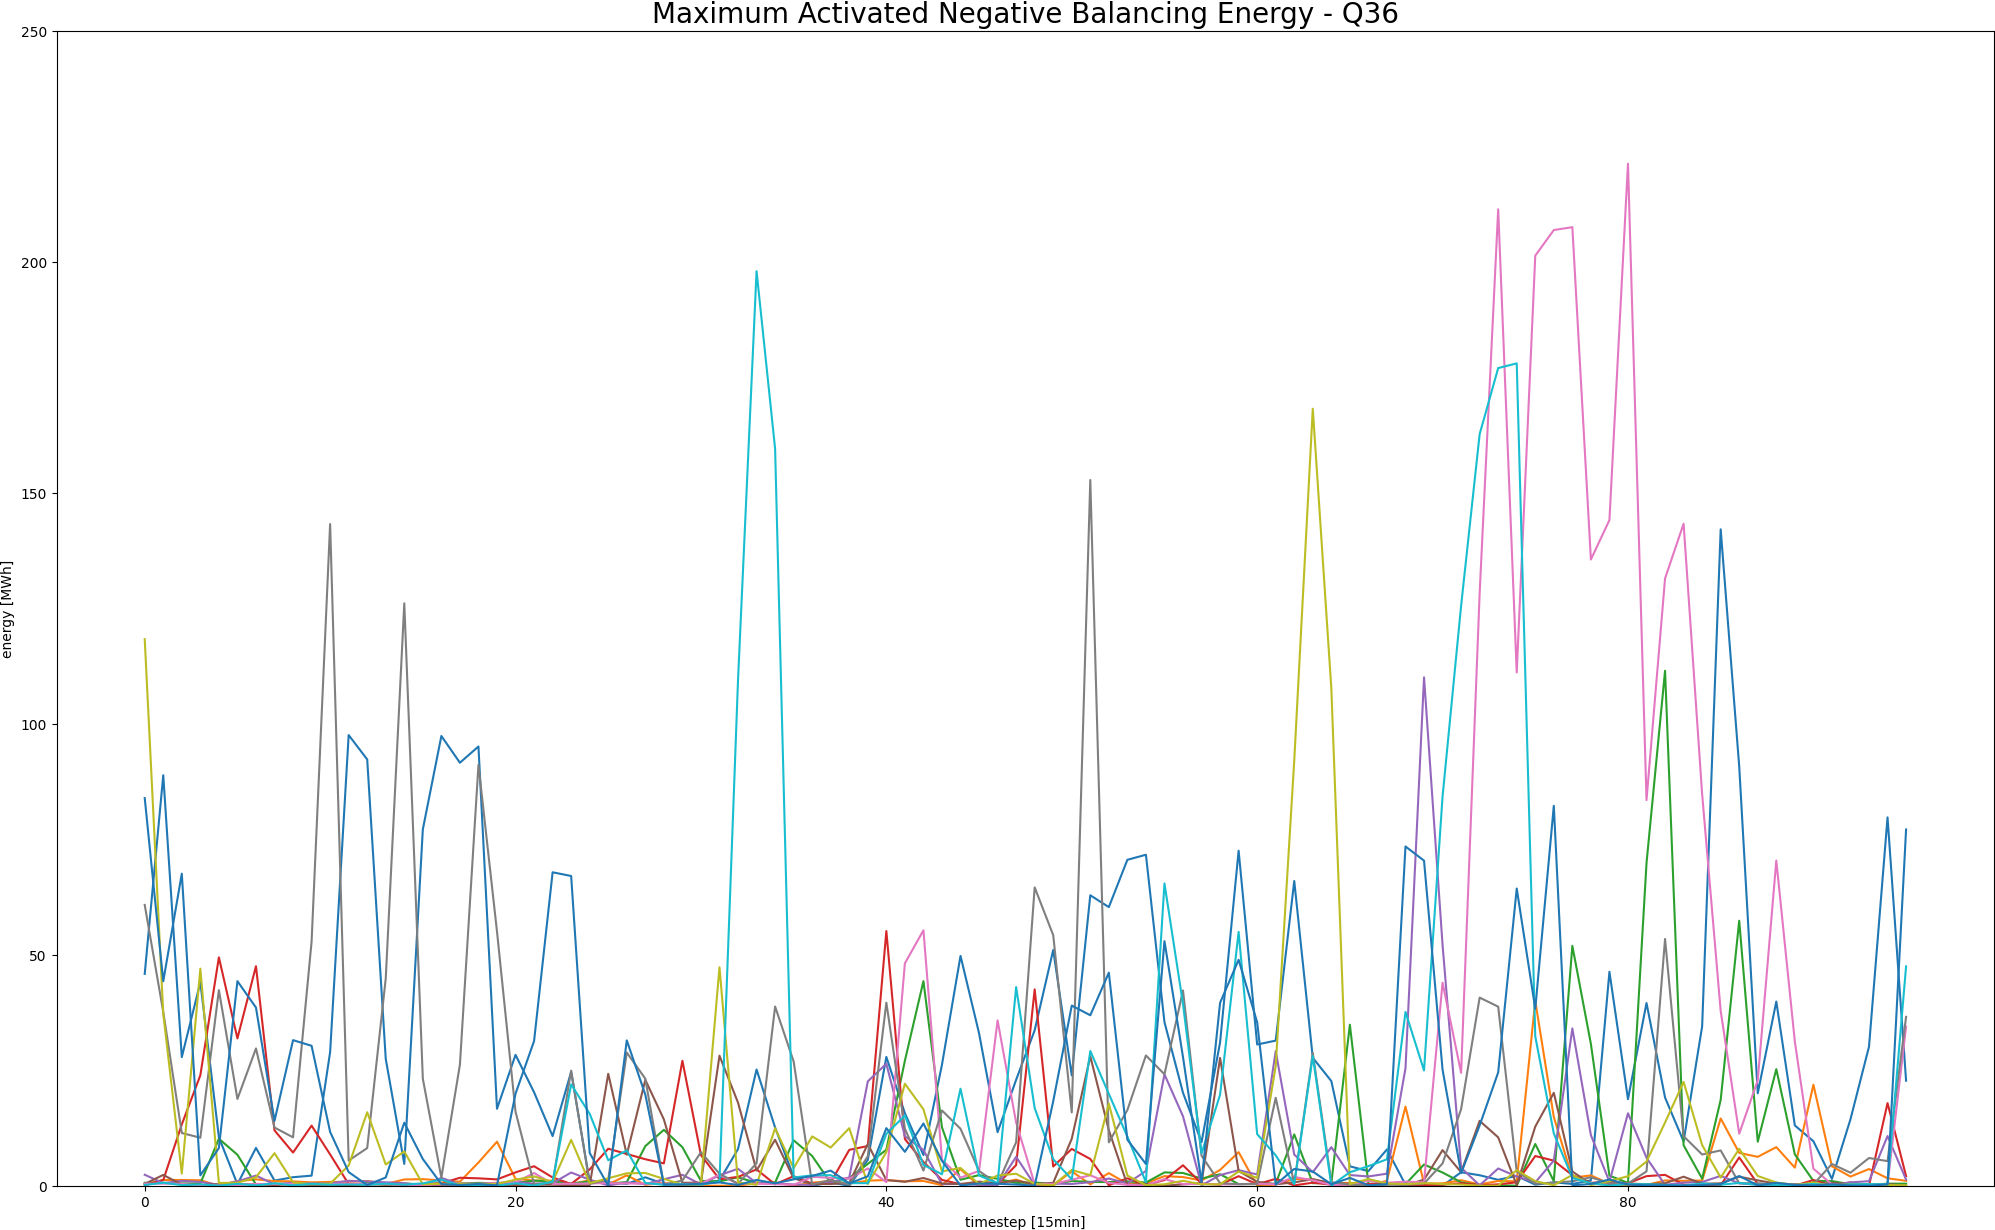
\includegraphics[width=1\linewidth]{pictures/results/Activated_negEnergy_Q36.png}
	\caption{Activated Negative Energy Q36}
	\label{fig:_negEnergy_Q36}
\end{figure}
\begin{figure}
	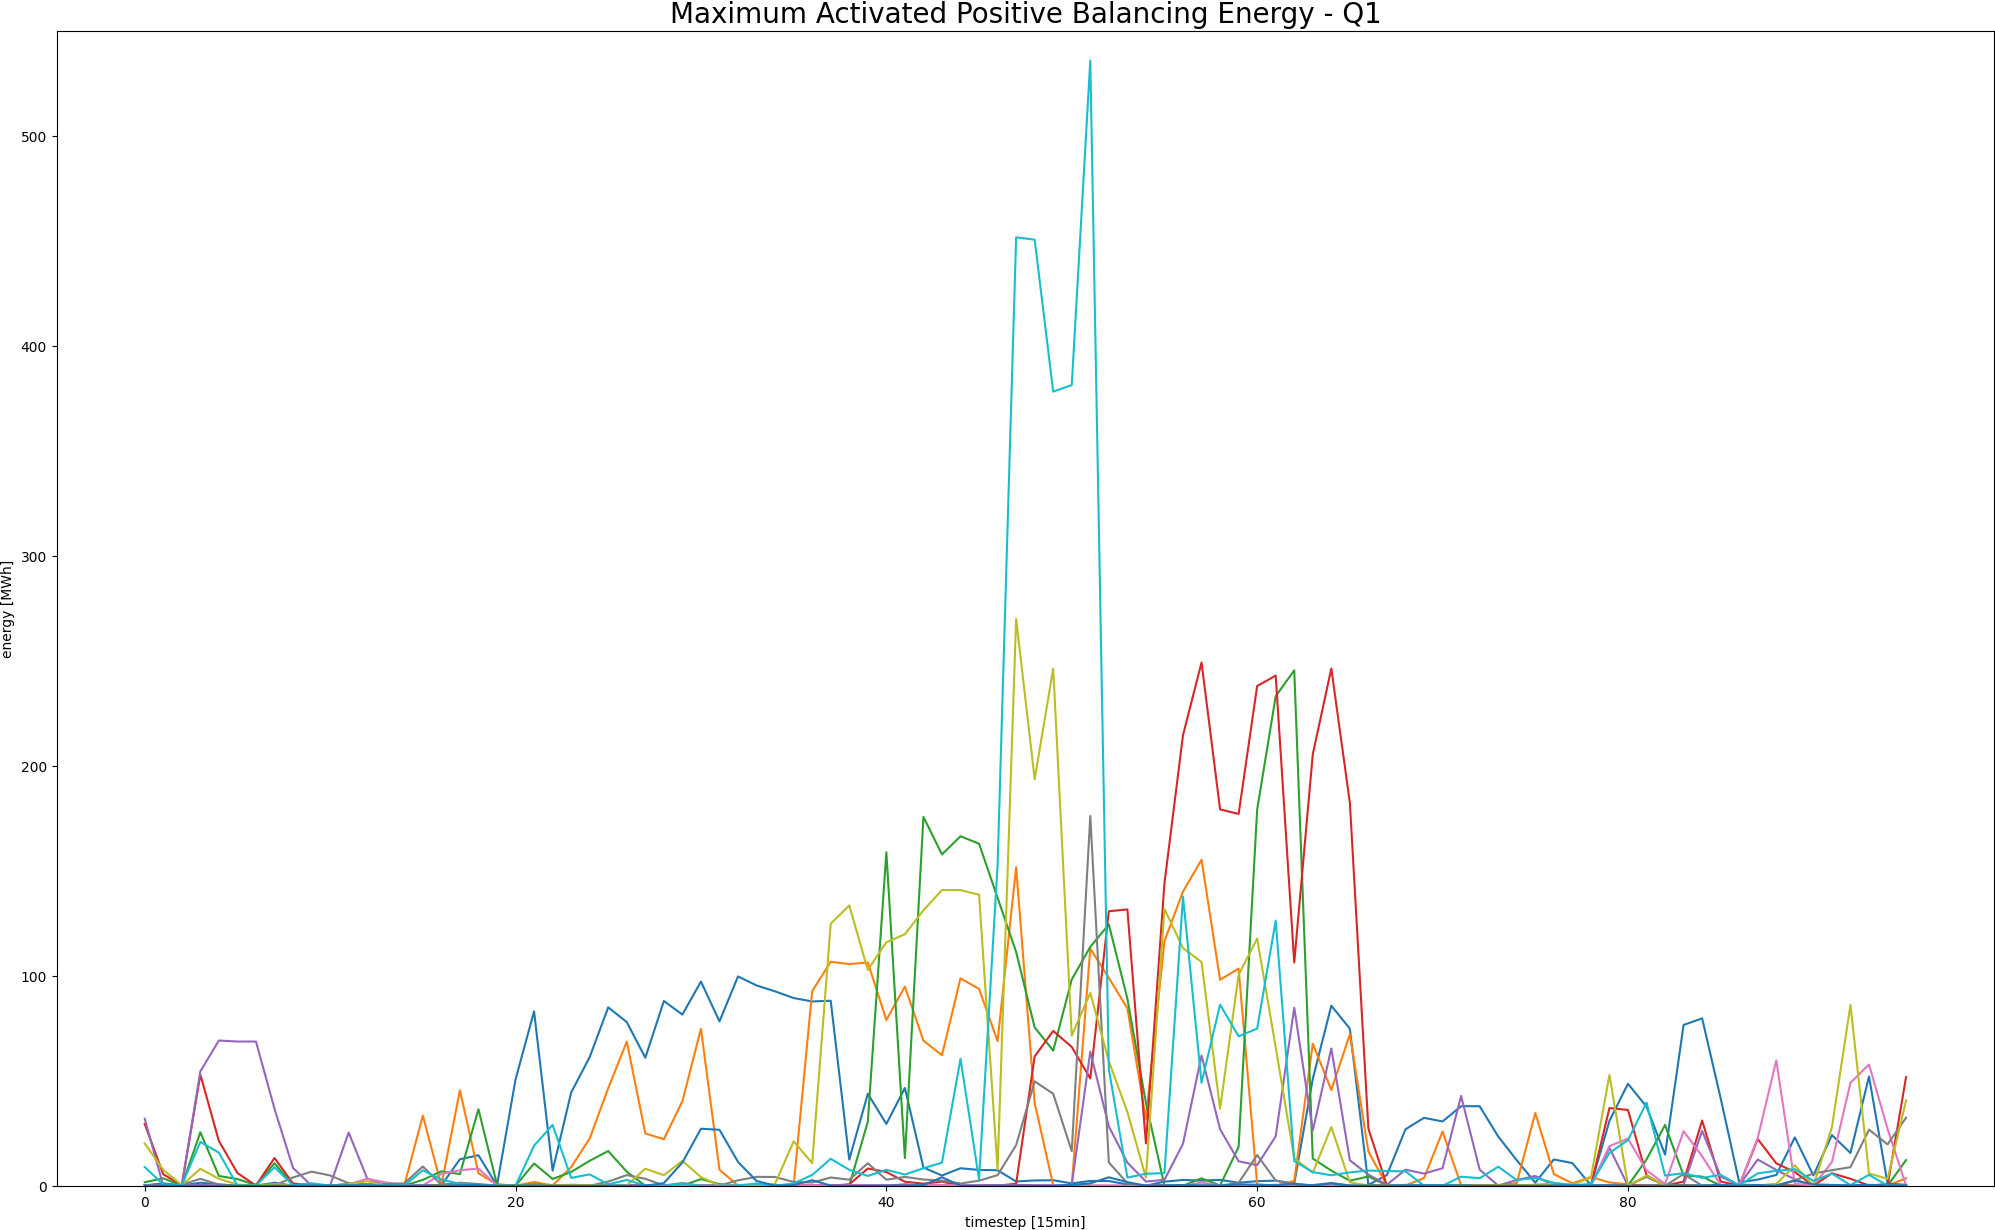
\includegraphics[width=1\linewidth]{pictures/results/Activated_posEnergy_Q1.png}
	\caption{Activated Positive Energy Q1}
	\label{fig:_posEnergy_Q1}
\end{figure}

\begin{figure}
	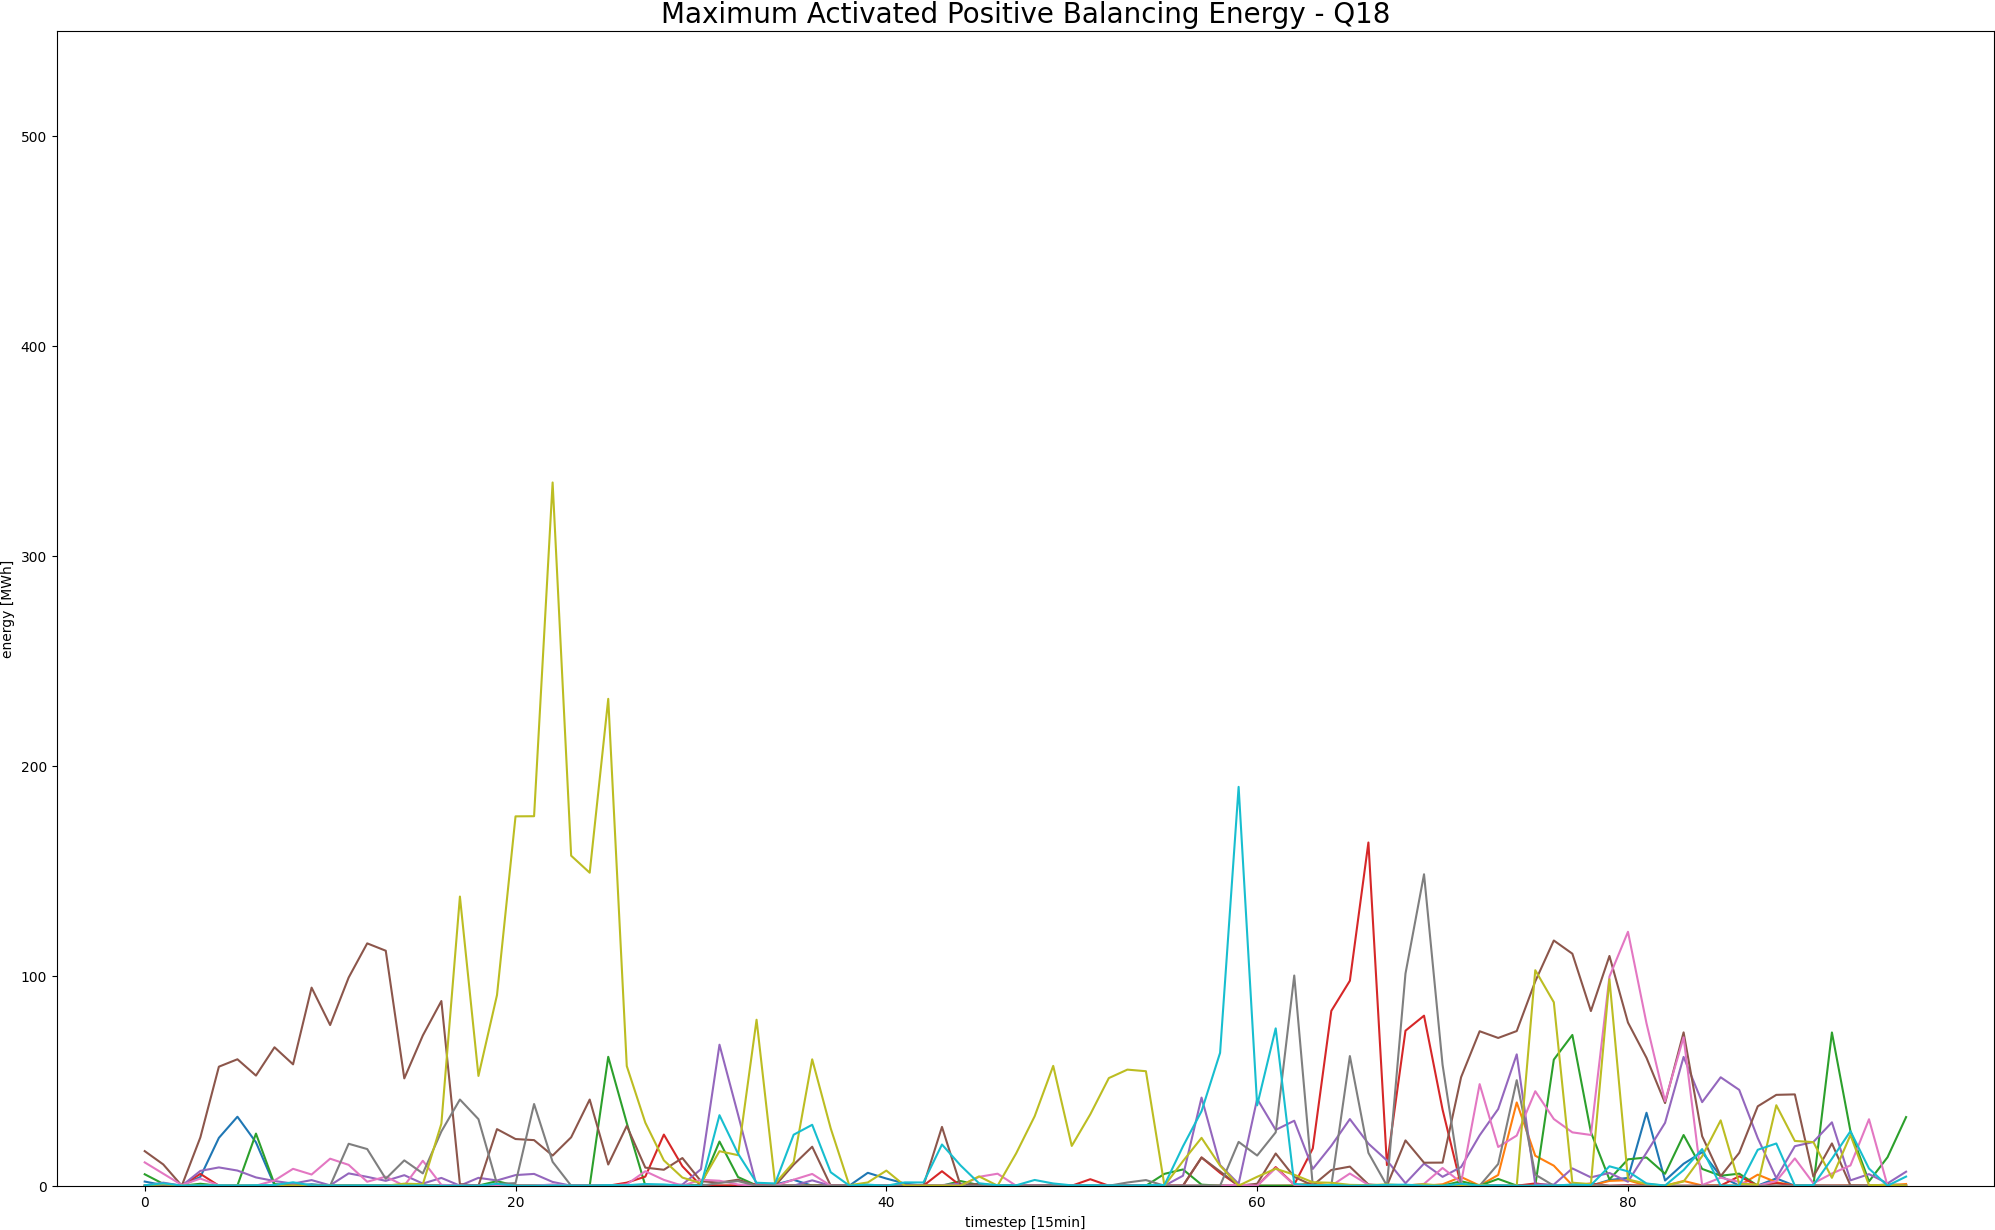
\includegraphics[width=1\linewidth]{pictures/results/Activated_posEnergy_Q18.png}
	\caption{Activated Positive Energy Q18}
	\label{fig:_posEnergy_Q18}
\end{figure}

\begin{figure}
	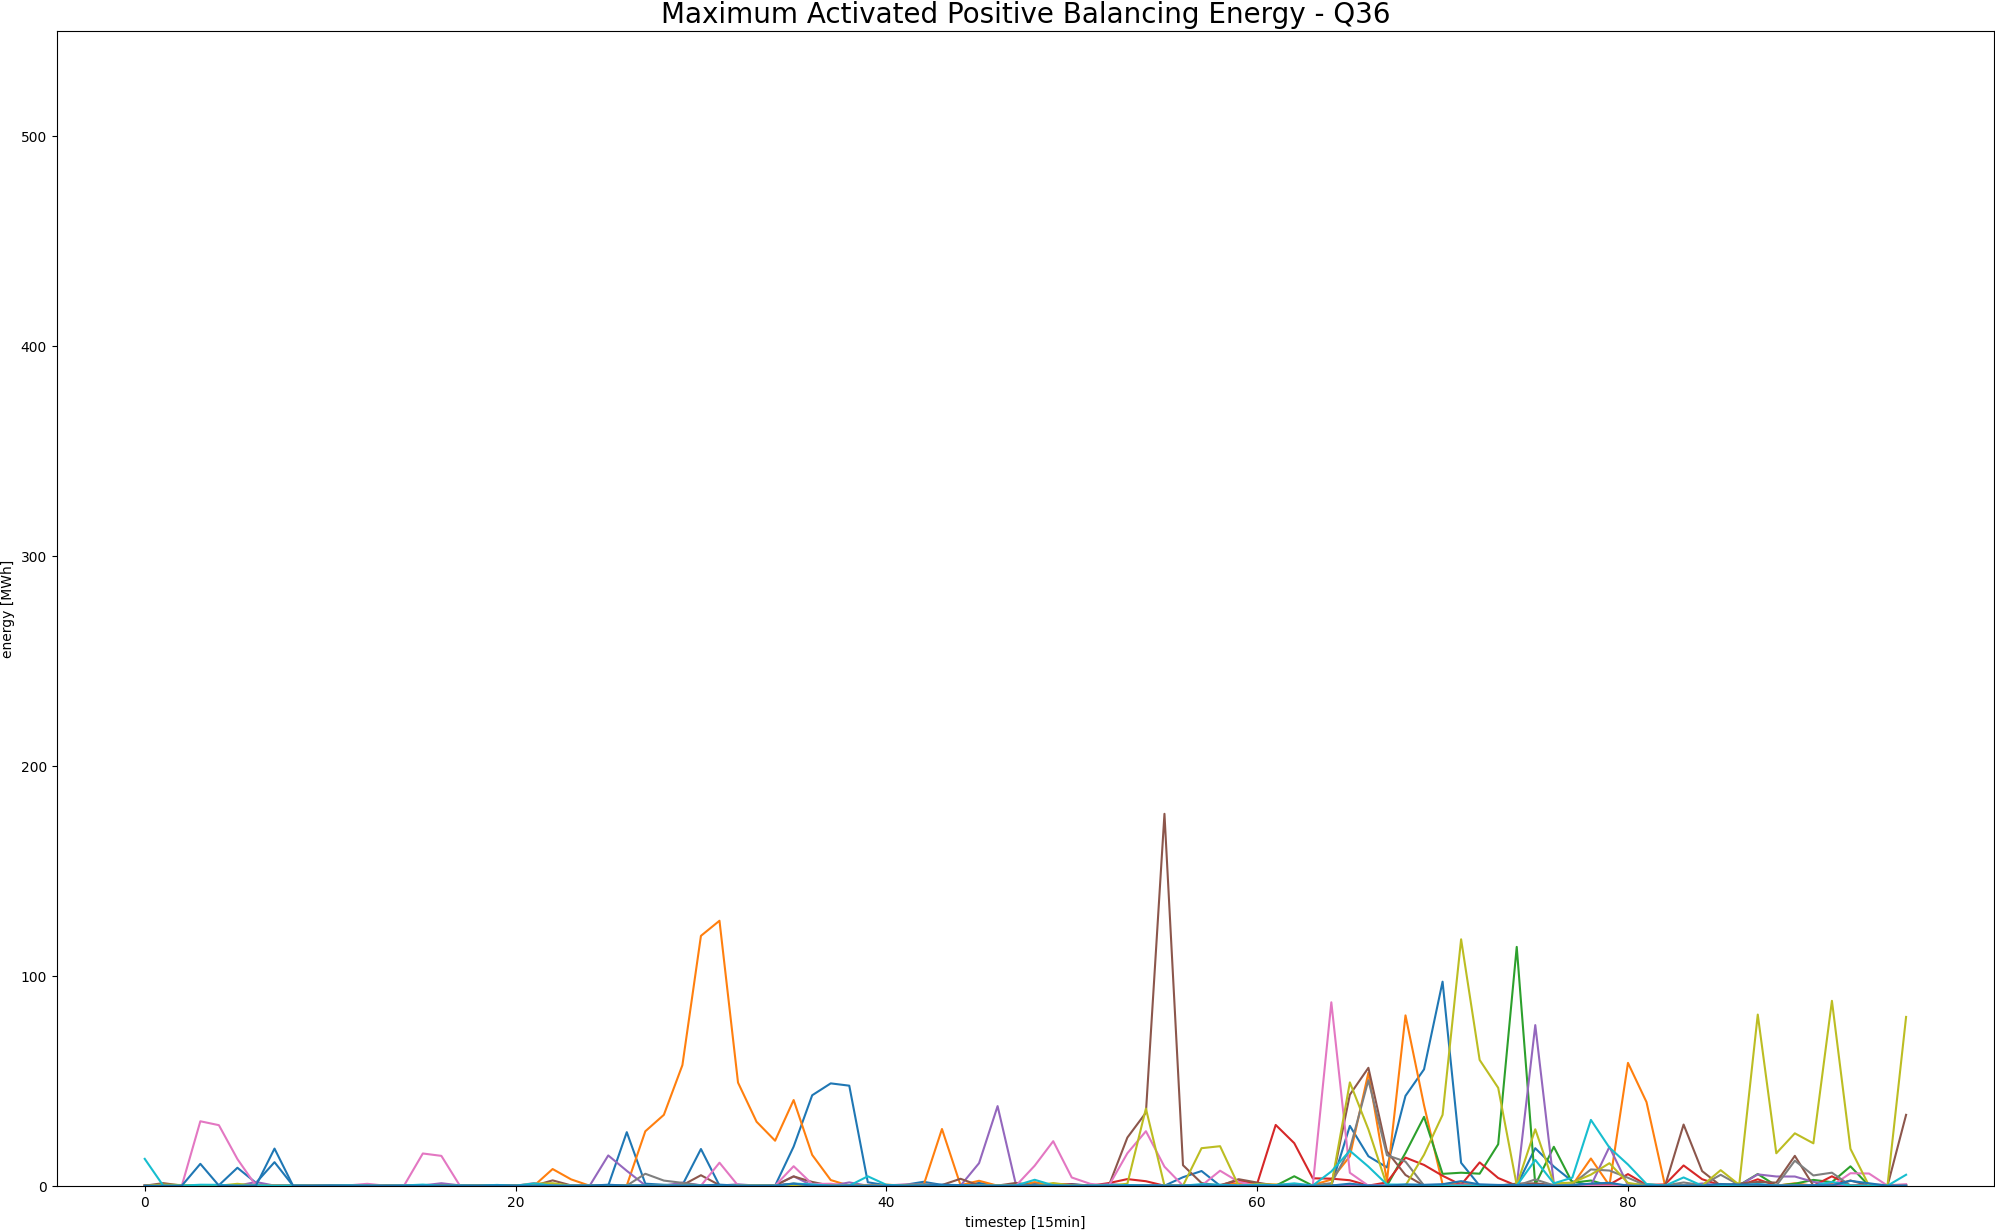
\includegraphics[width=1\linewidth]{pictures/results/Activated_posEnergy_Q36.png}
	\caption{Activated Positive Energy Q36}
	\label{fig:_posEnergy_Q36}
\end{figure}



\begin{figure}[H]
	\centering
	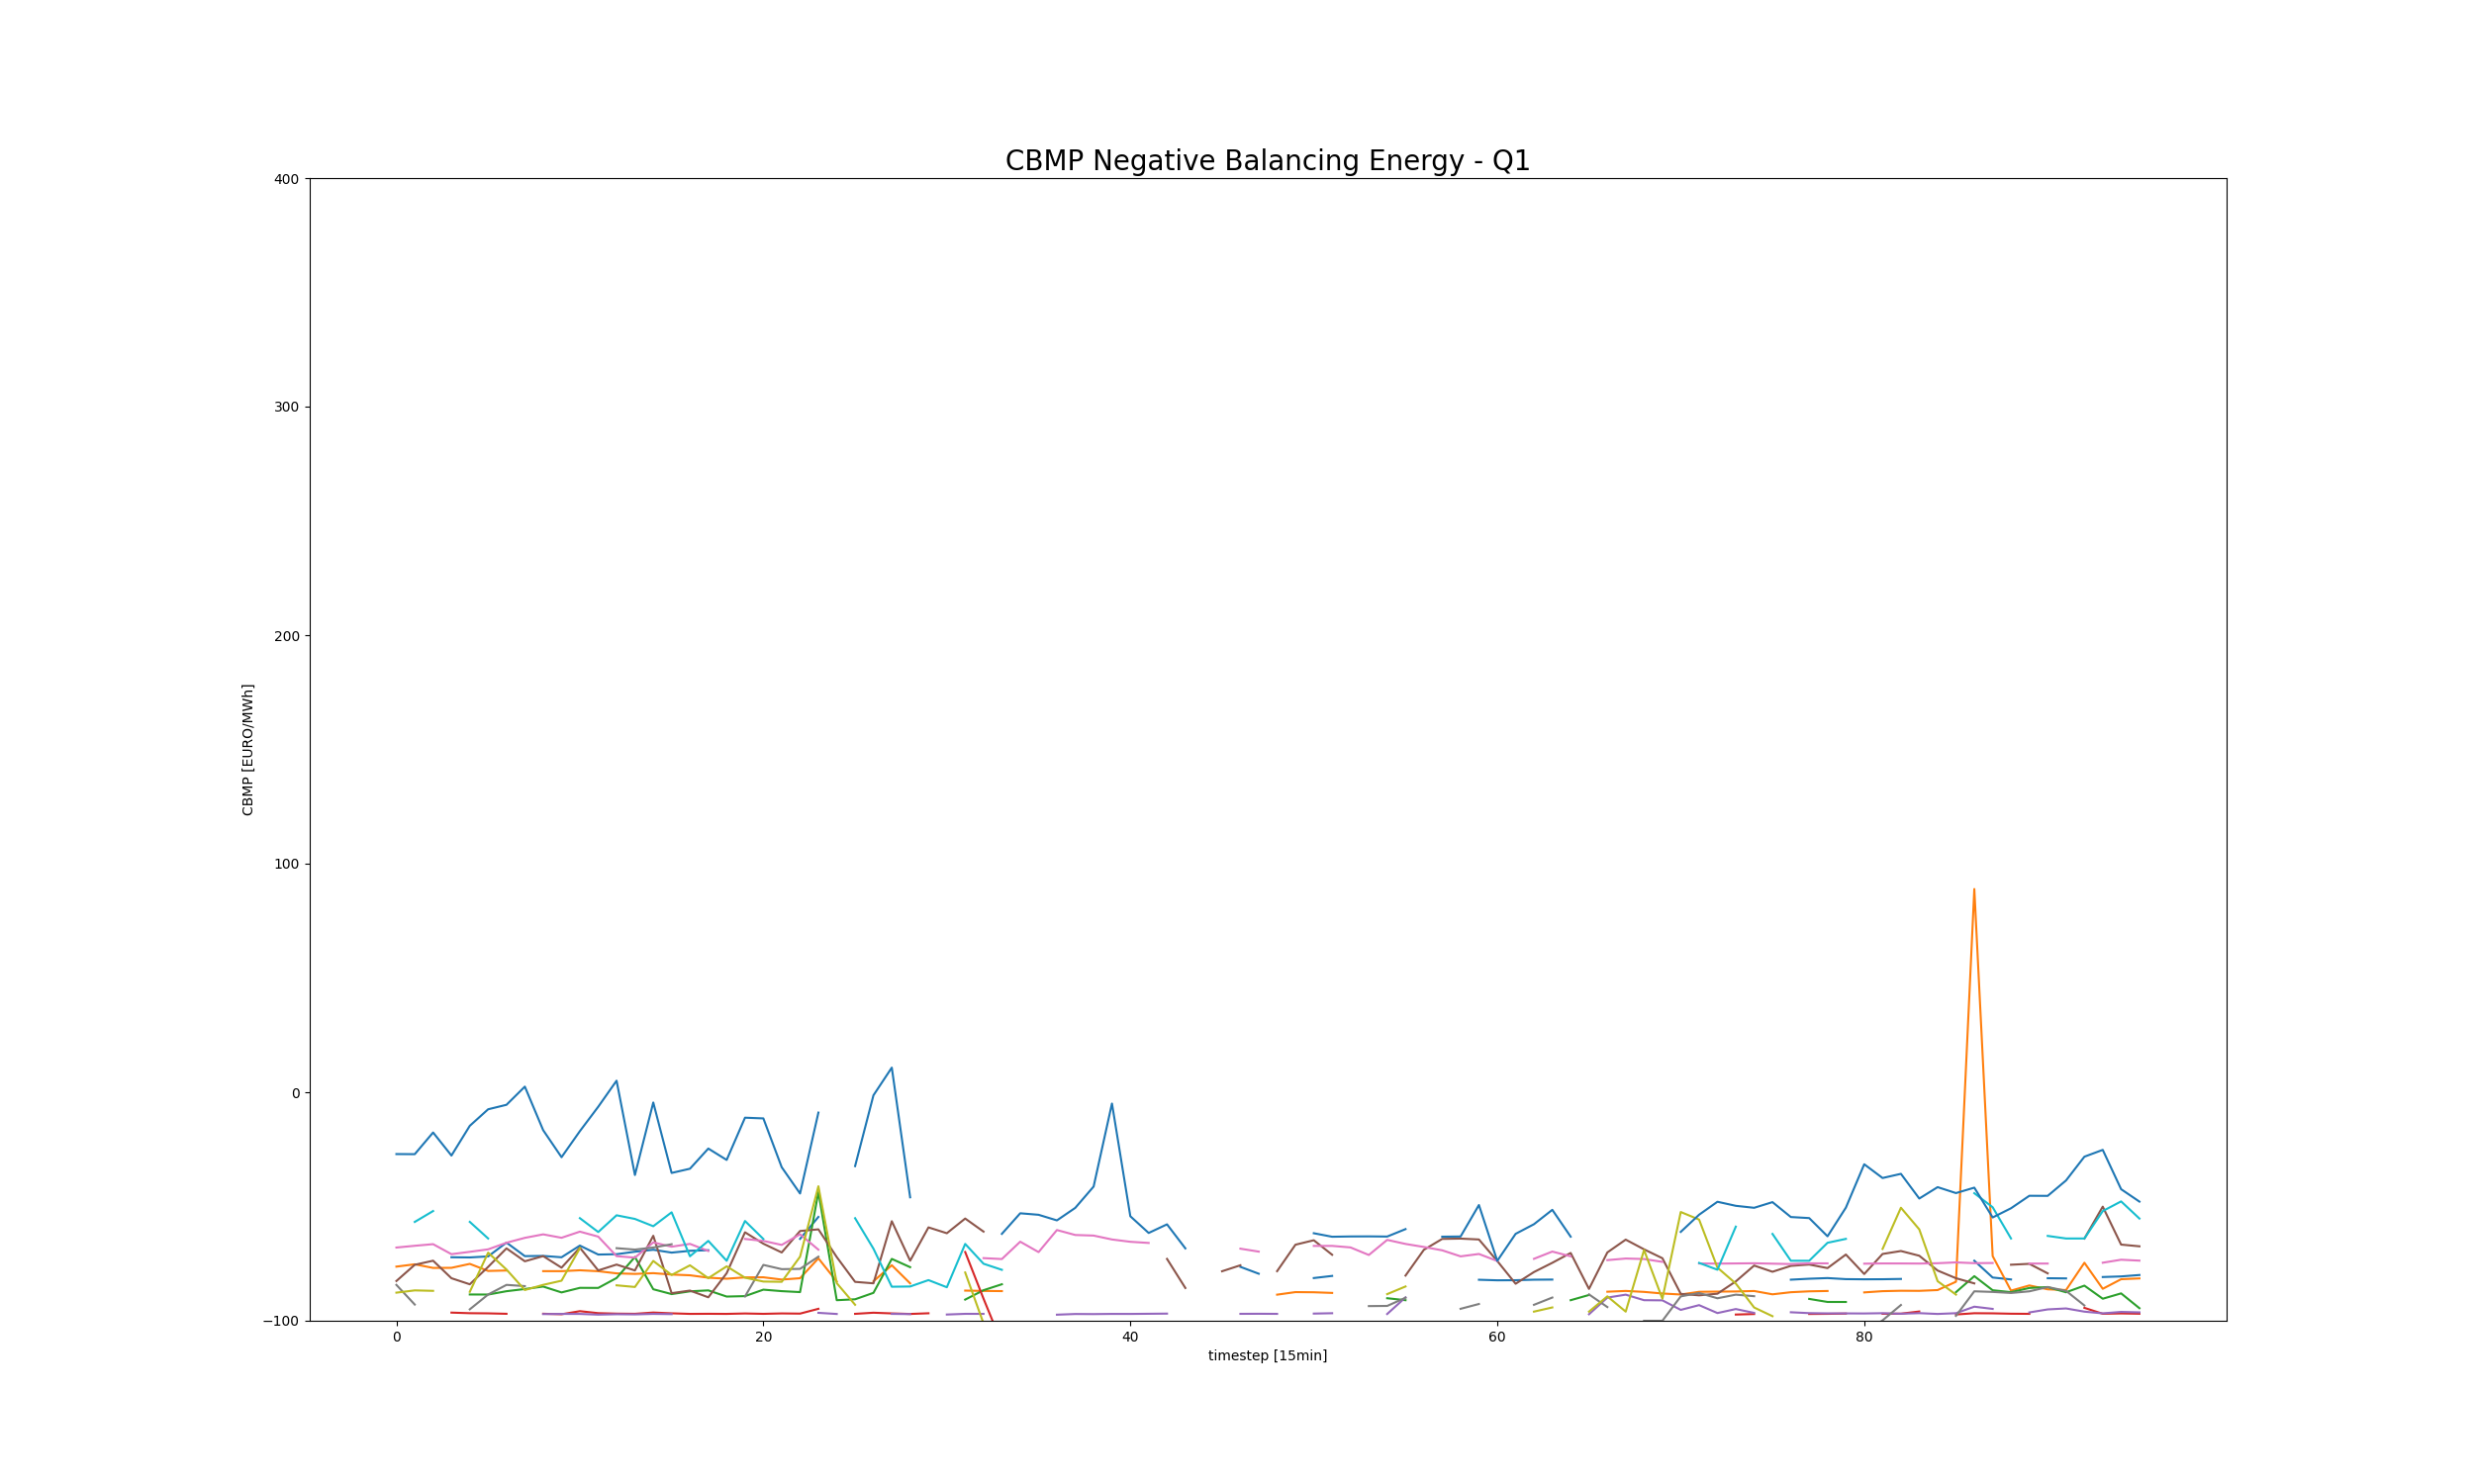
\includegraphics[width=1\linewidth]{pictures/results/CBMP_negBal_Q1.png}
	\caption{CBMP Negative Energy Q1}
	\label{fig:CBMP_negBal_Q1}
\end{figure}


\begin{figure}[H]
	\centering
	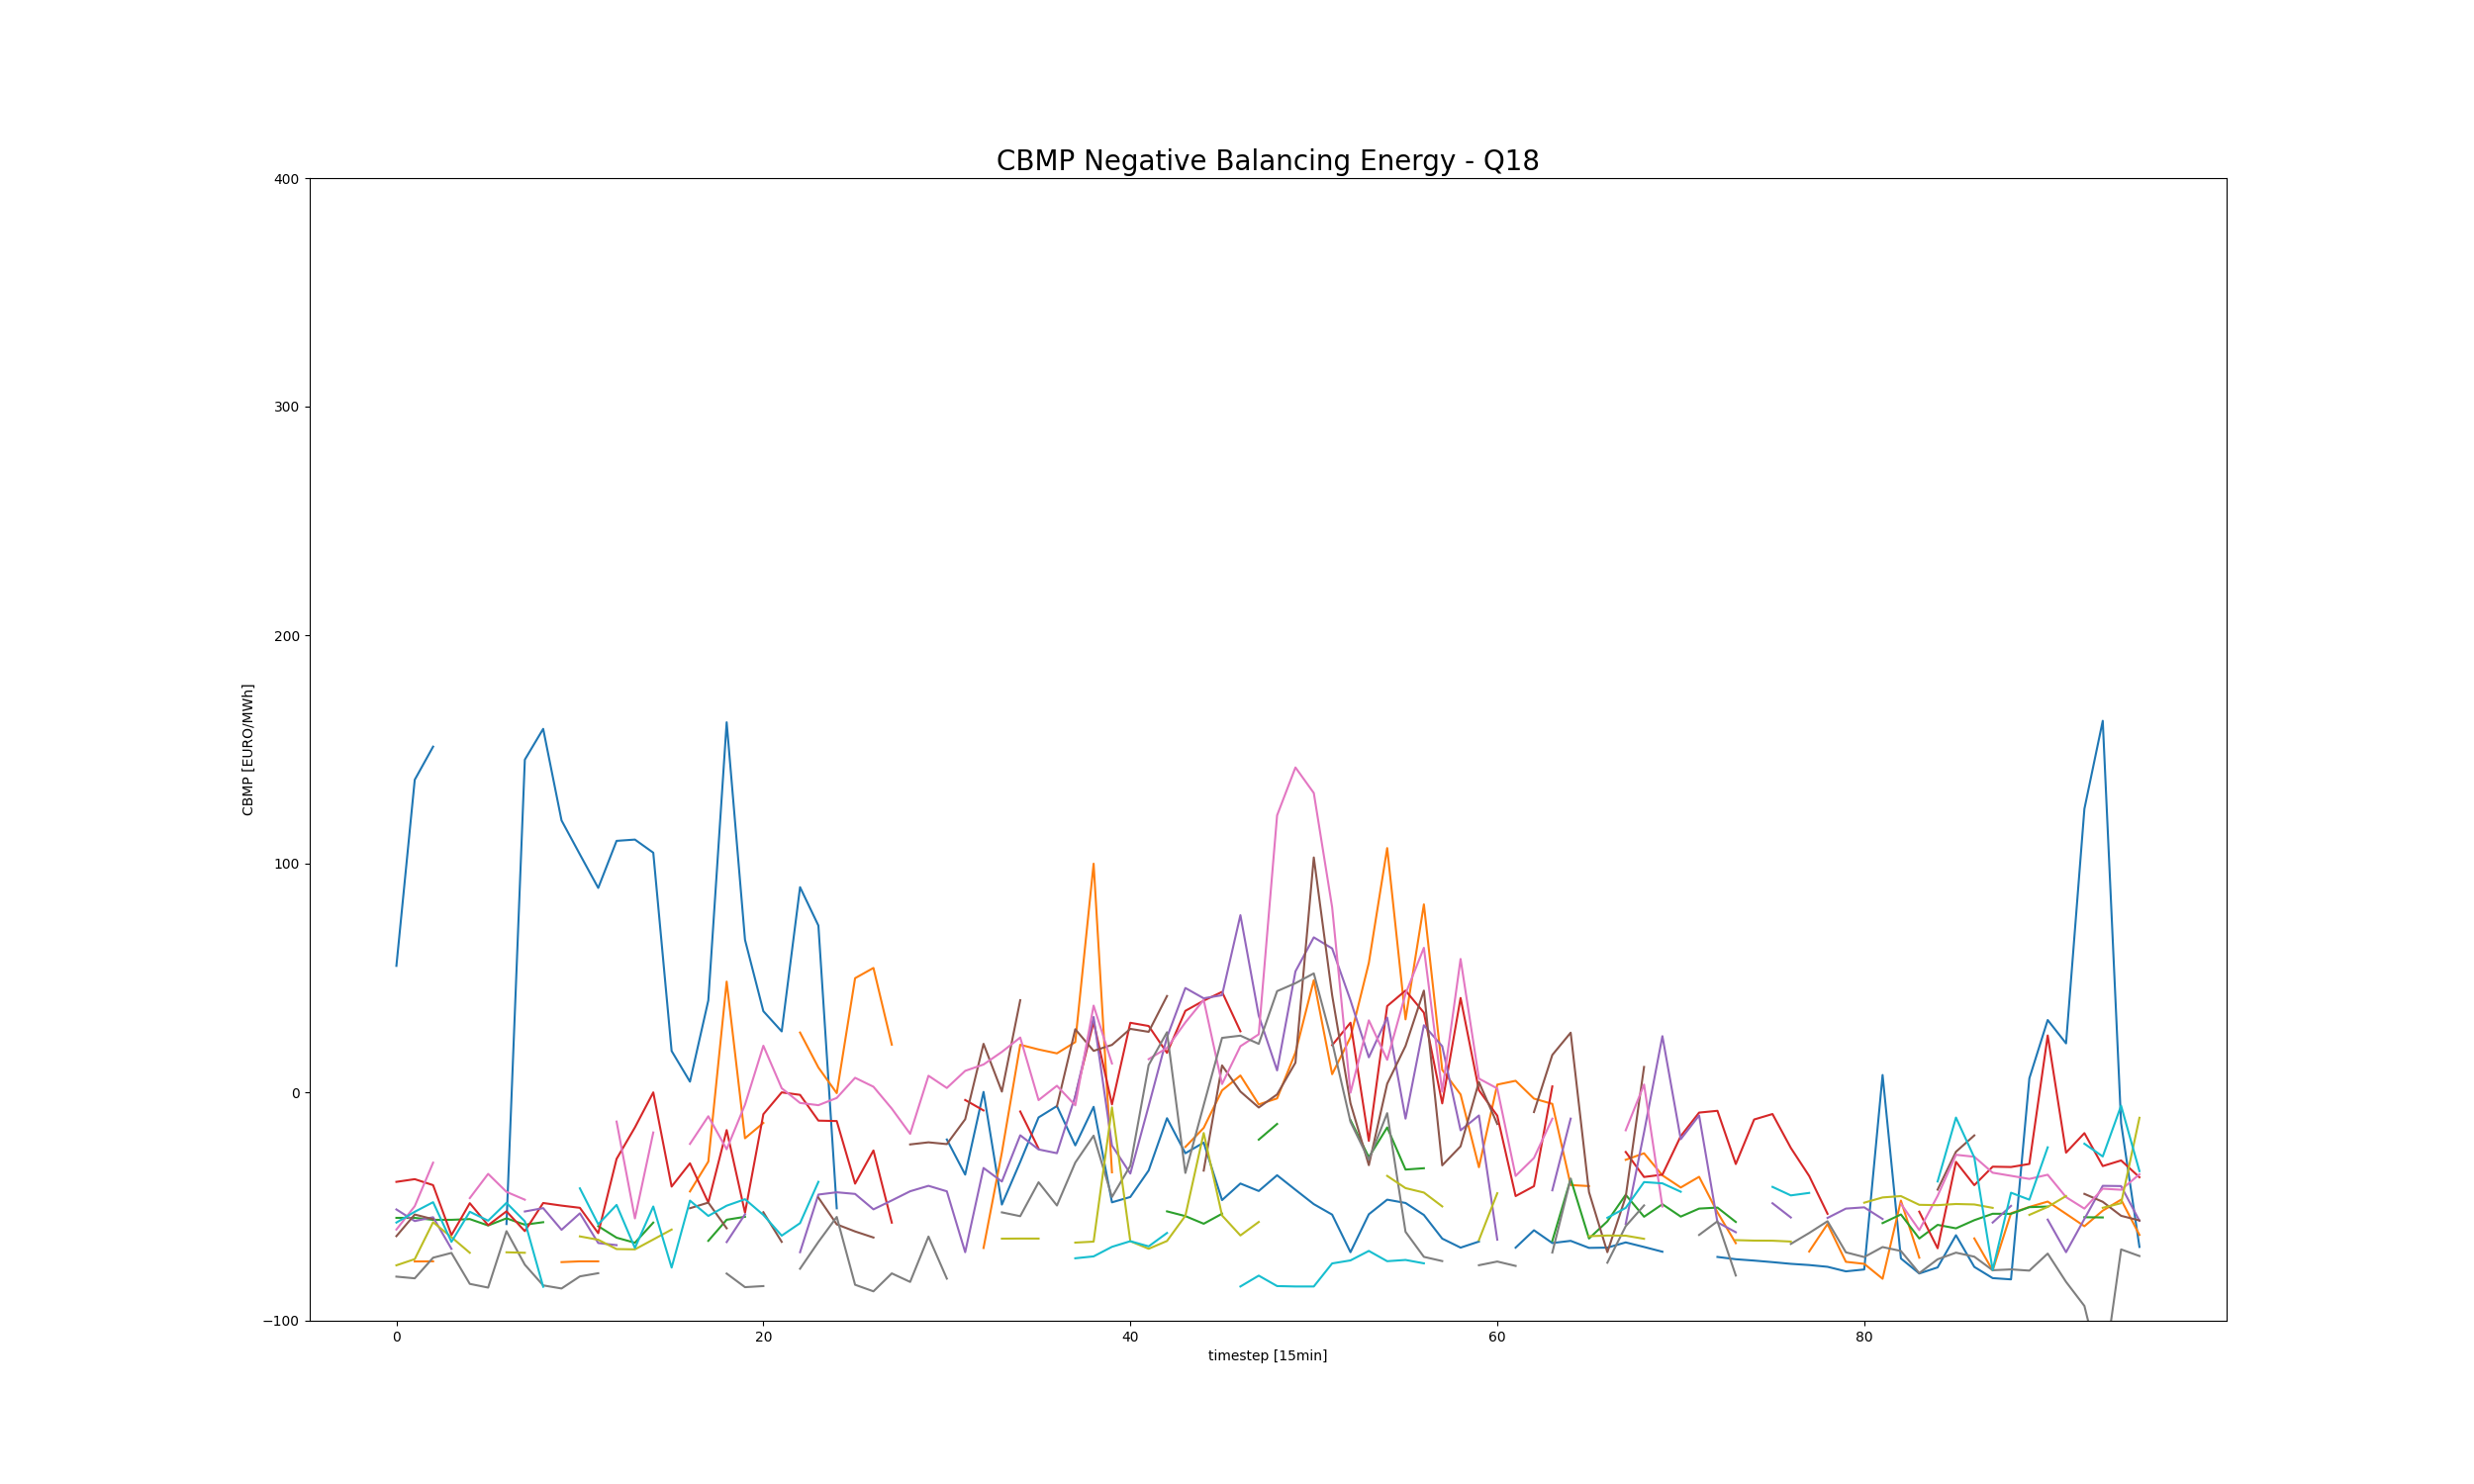
\includegraphics[width=1\linewidth]{pictures/results/CBMP_negBal_Q18.png}
	\caption{CBMP Negative Energy Q18}
	\label{fig:CBMP_negBal_Q18}
\end{figure}


\begin{figure}[H]
	\centering
	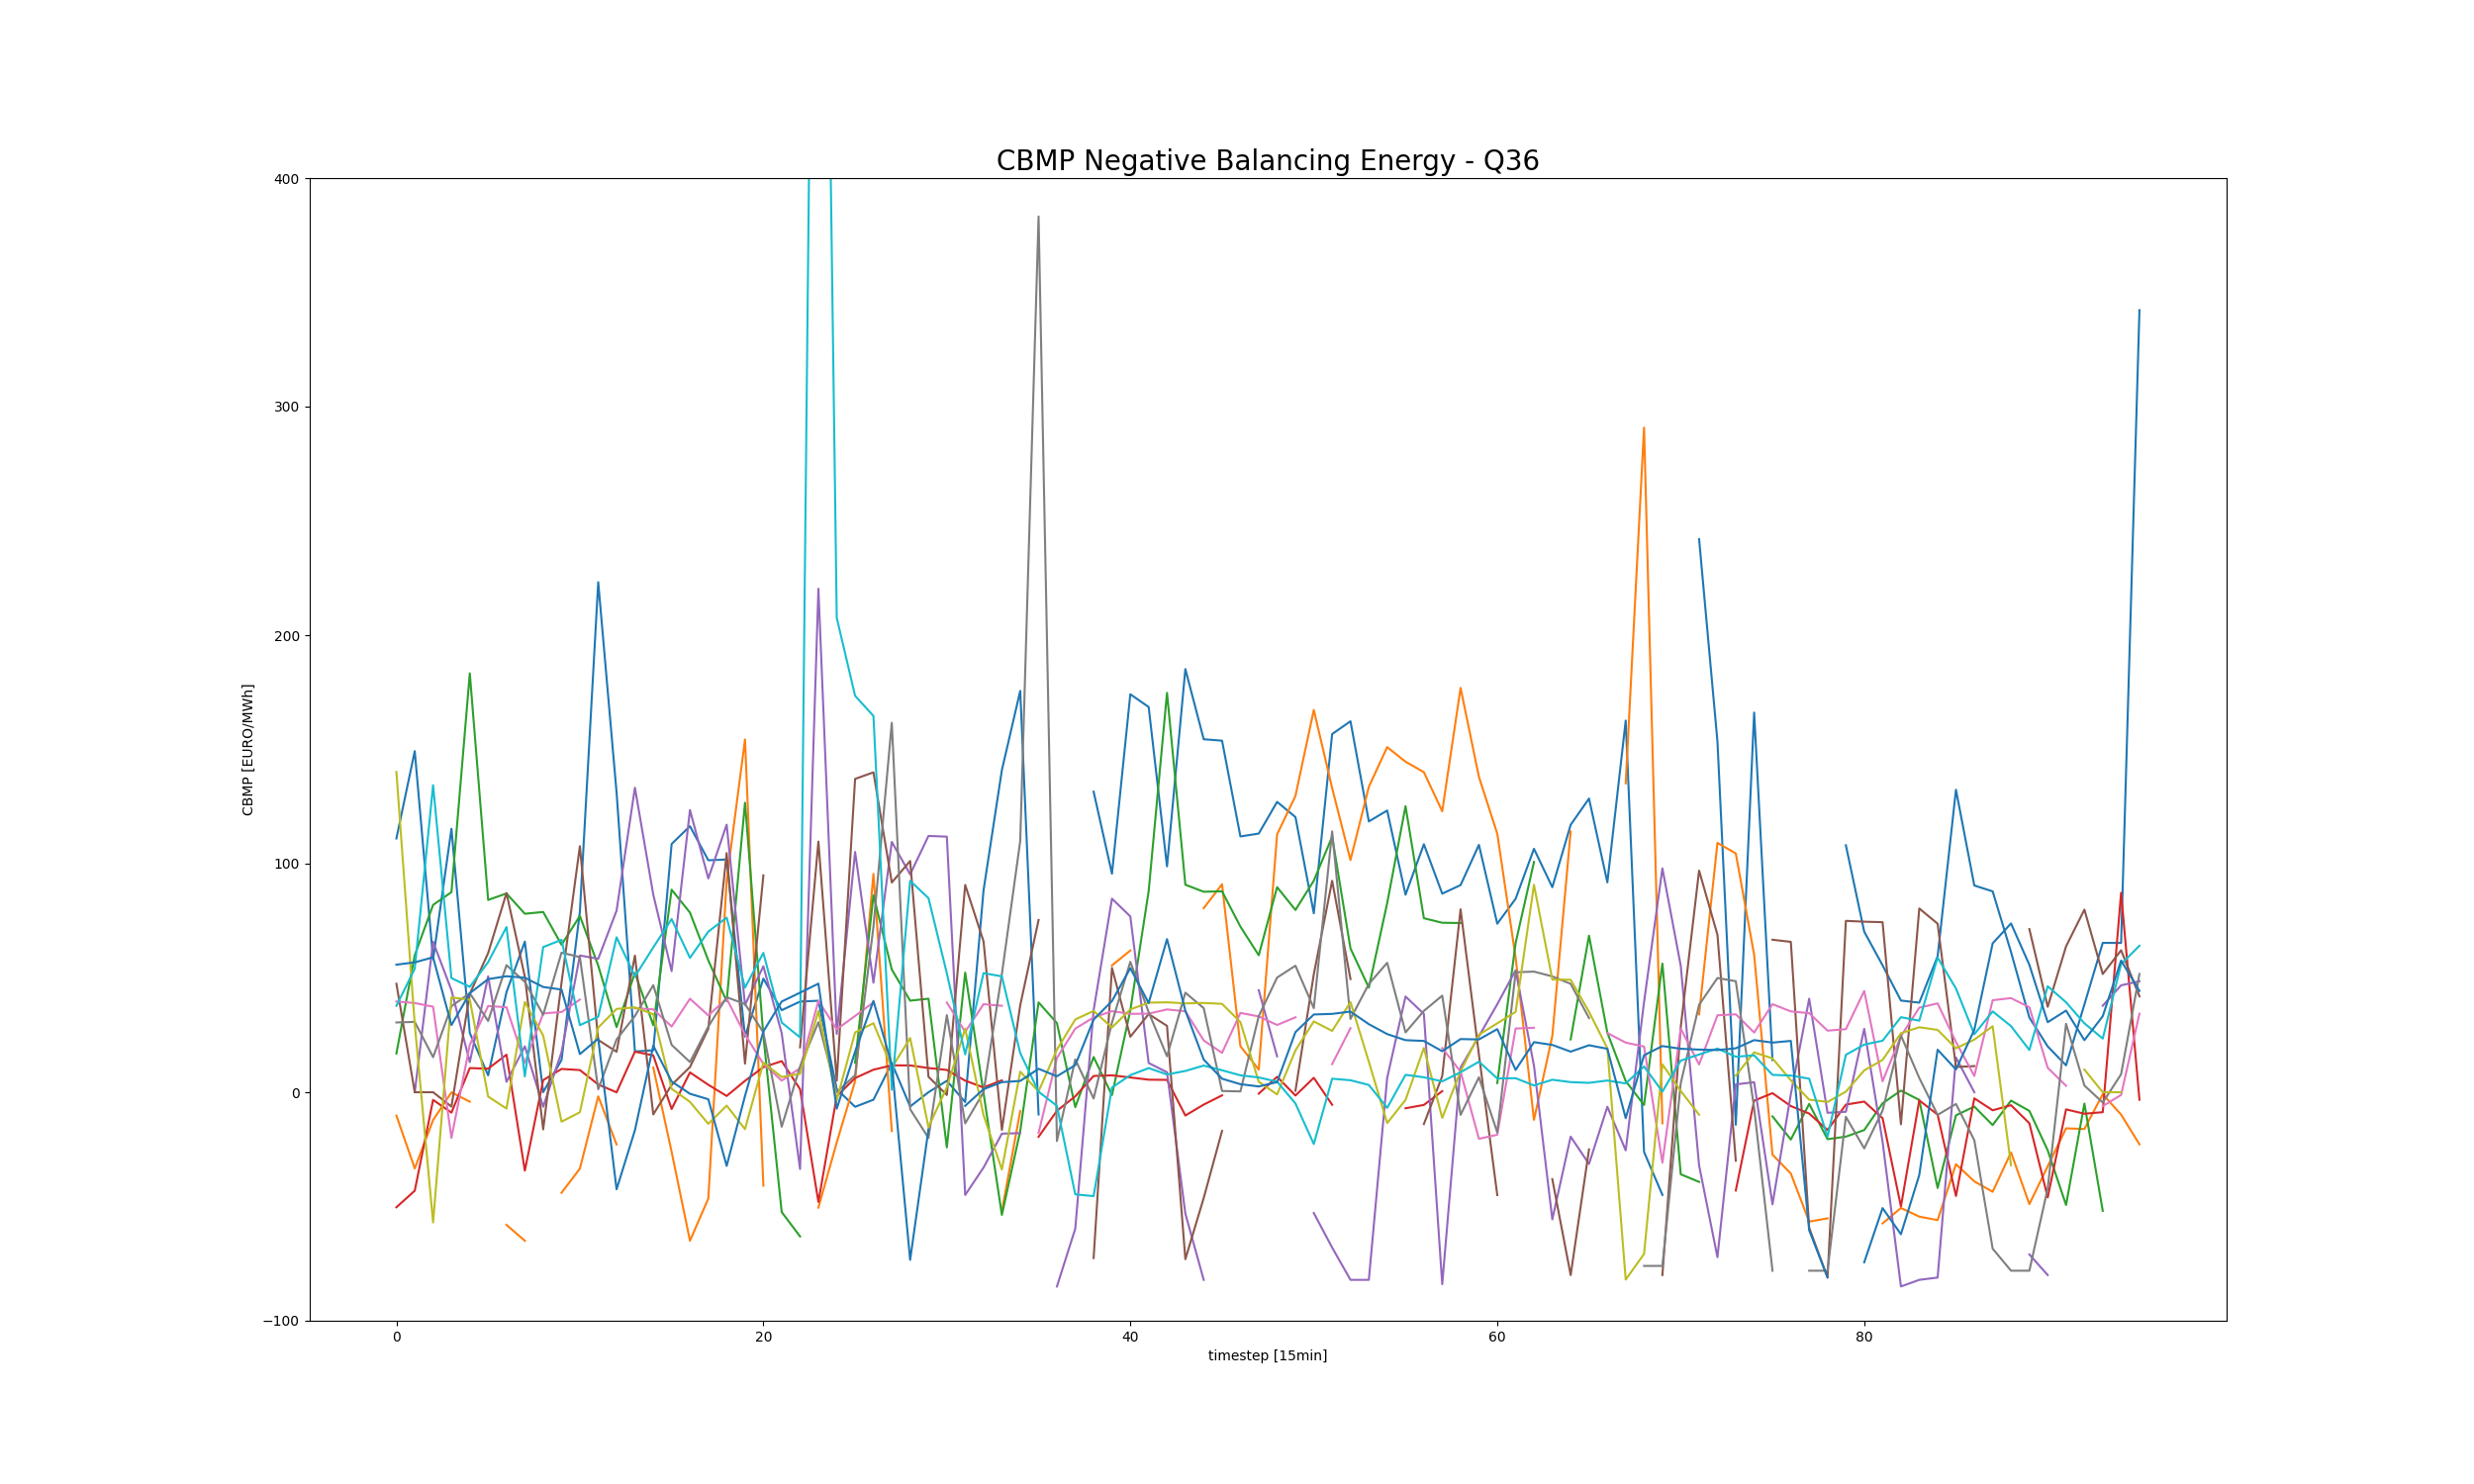
\includegraphics[width=1\linewidth]{pictures/results/CBMP_negBal_Q36.png}
	\caption{CBMP Negative Energy Q36}
	\label{fig:CBMP_negBal_Q36}
\end{figure}

\begin{figure}
	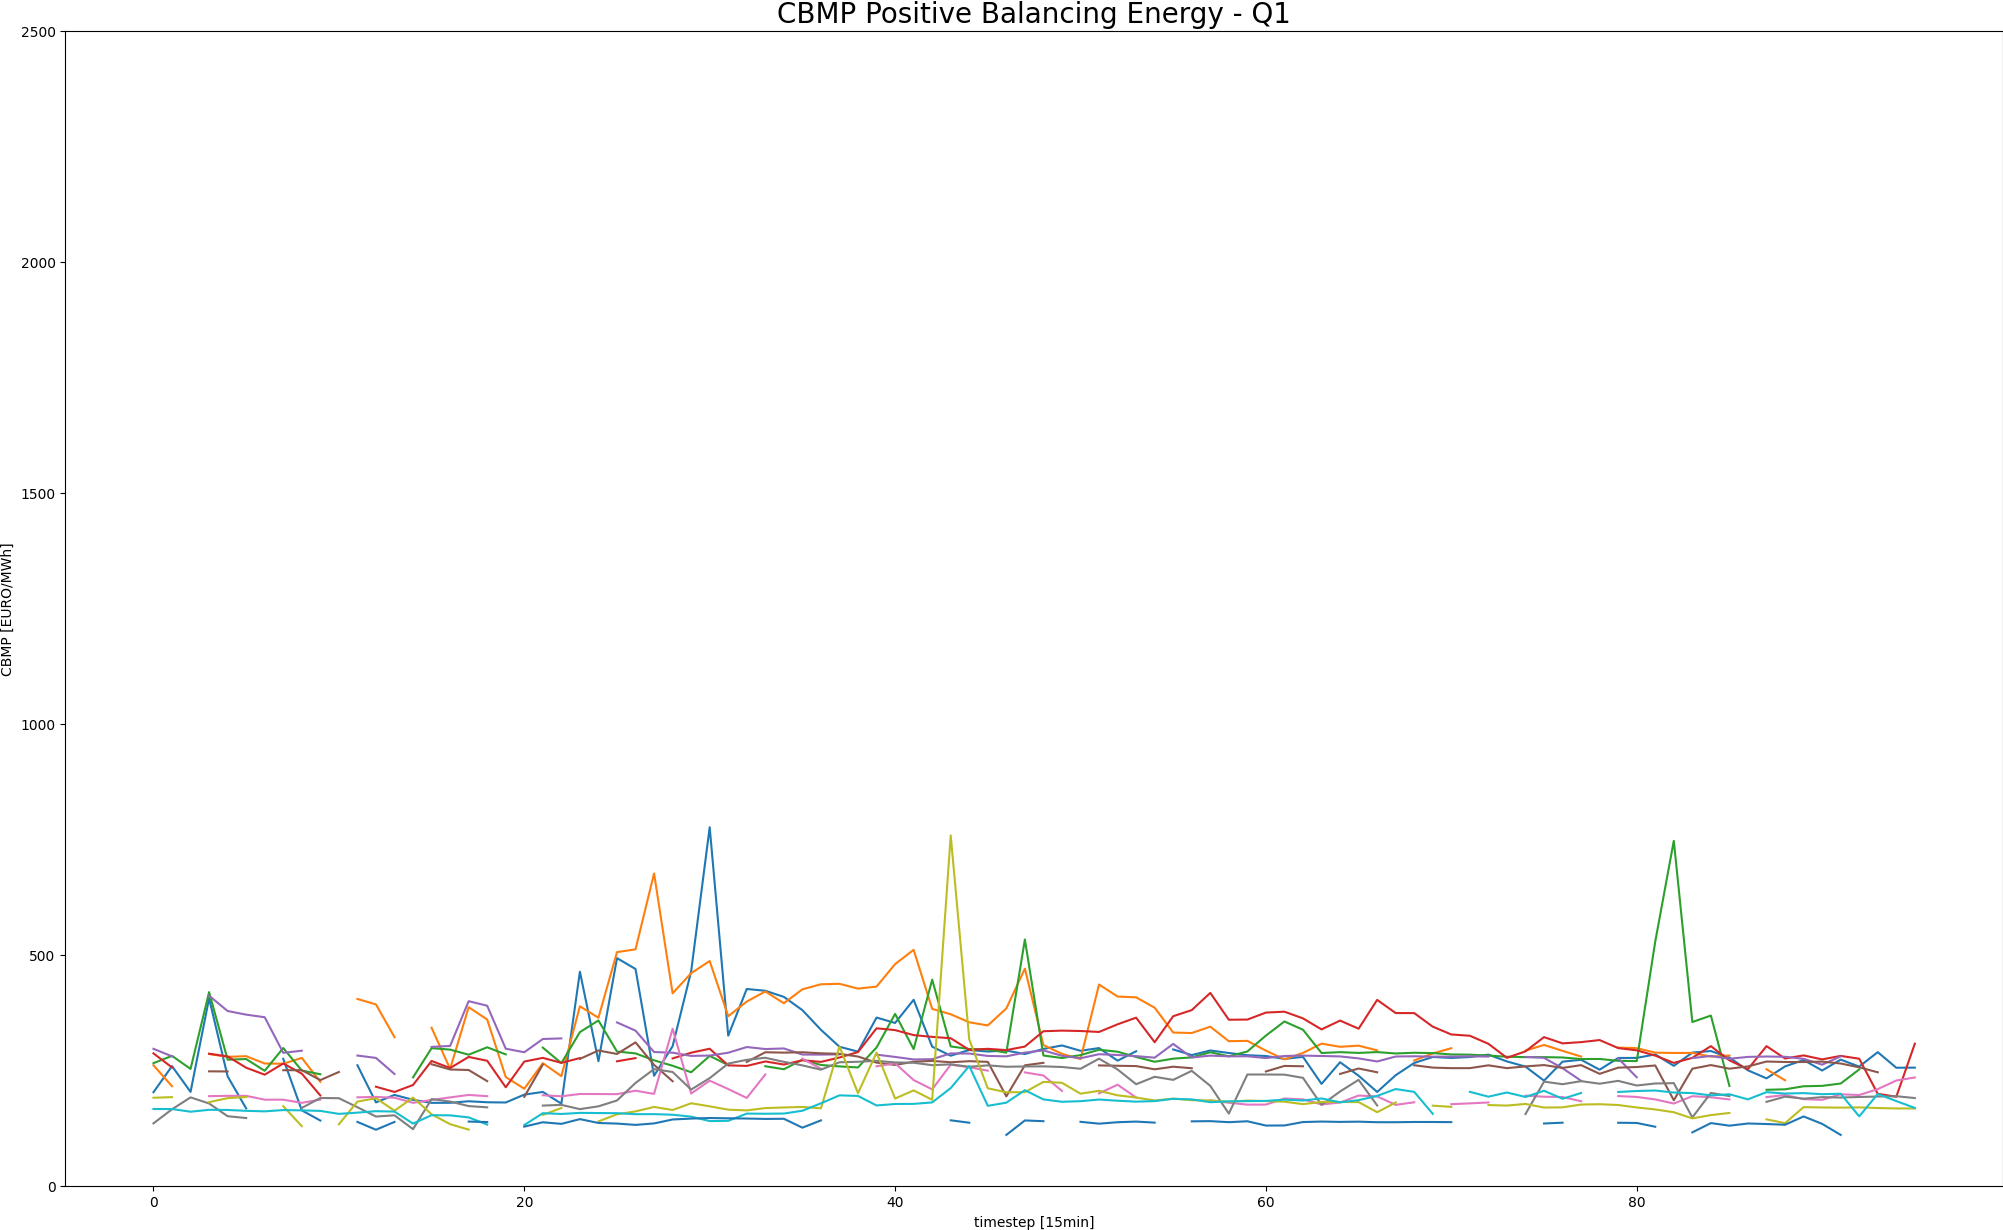
\includegraphics[width=1\linewidth]{pictures/results/CBMP_PosBal_Q1.png}
	\caption{CBMP Positive Energy Q1}
	\label{fig:CBMP_PosBal_Q1}
\end{figure}

\begin{figure}
	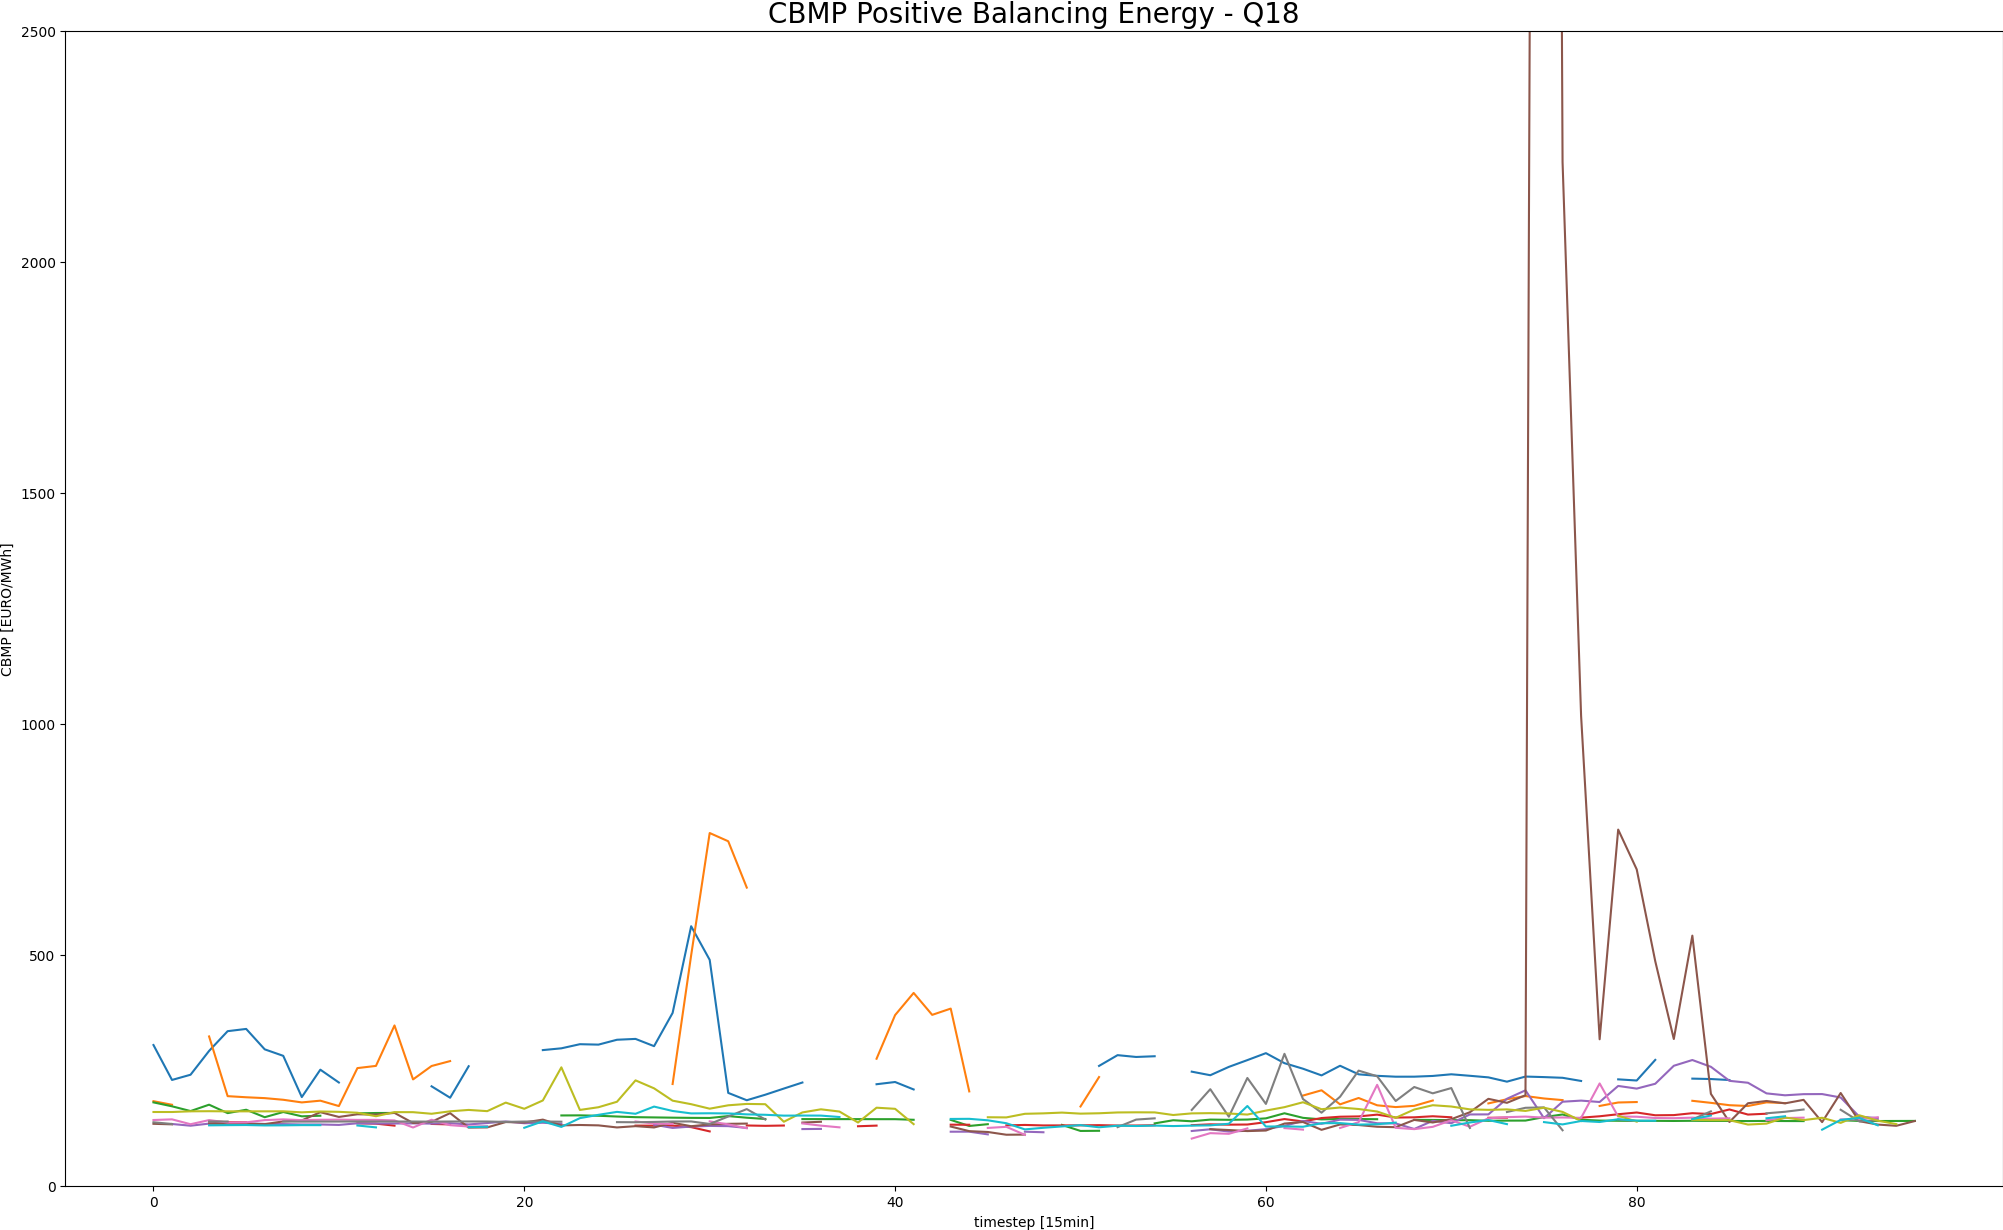
\includegraphics[width=1\linewidth]{pictures/results/CBMP_PosBal_Q18.png}
	\caption{CBMP Positive Energy Q18}
	\label{fig:CBMP_PosBal_Q18}
\end{figure}
\begin{figure}
	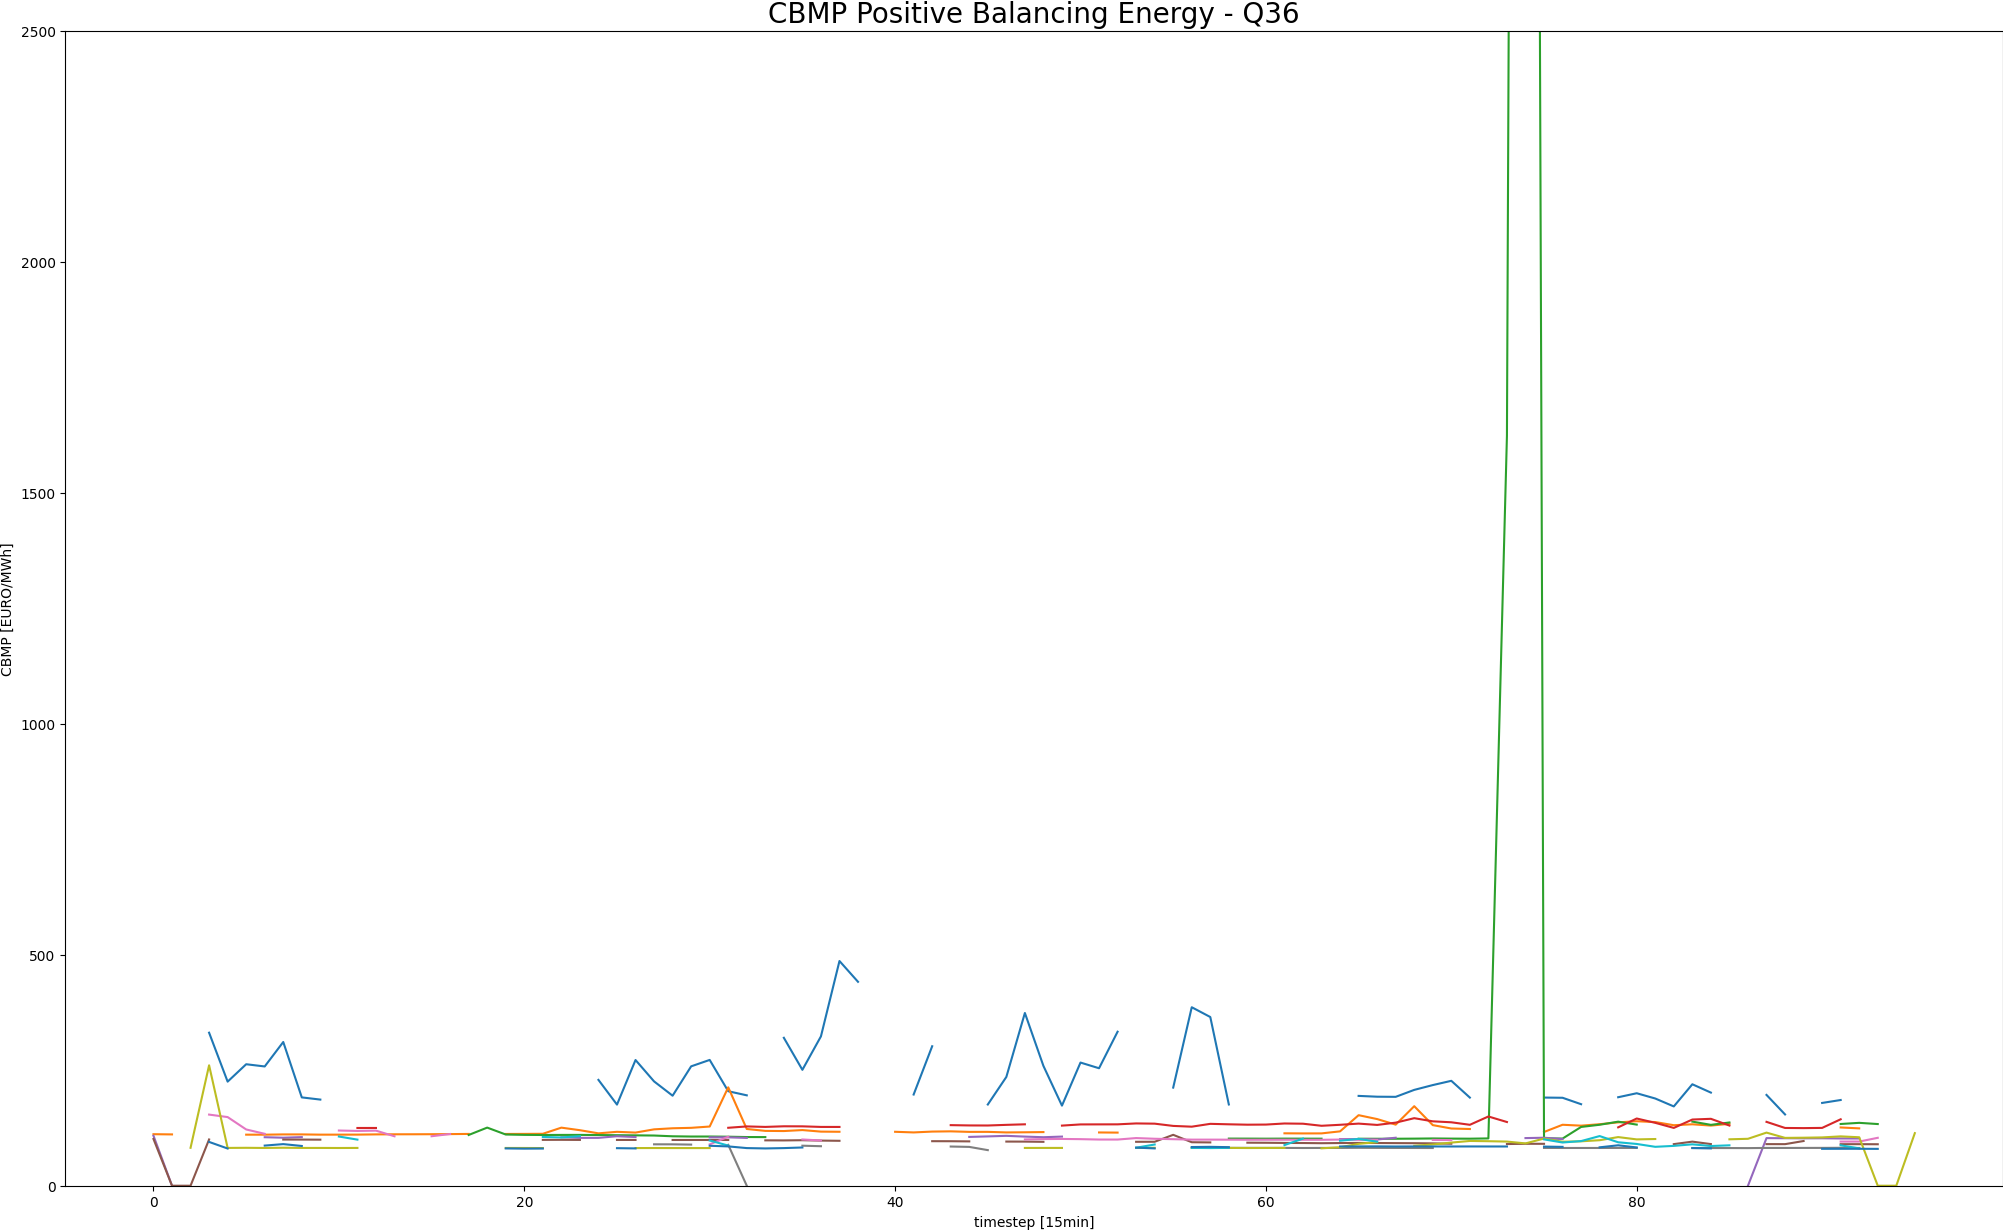
\includegraphics[width=1\linewidth]{pictures/results/CBMP_PosBal_Q36.png}
	\caption{CBMP Positive Energy Q36}
	\label{fig:CBMP_PosBal_Q36}
\end{figure}

Für den selben Zeitabschnitt lässt sich der DA Markt wie folgt zusammenfassen:
\begin{figure}[H]
	\centering
	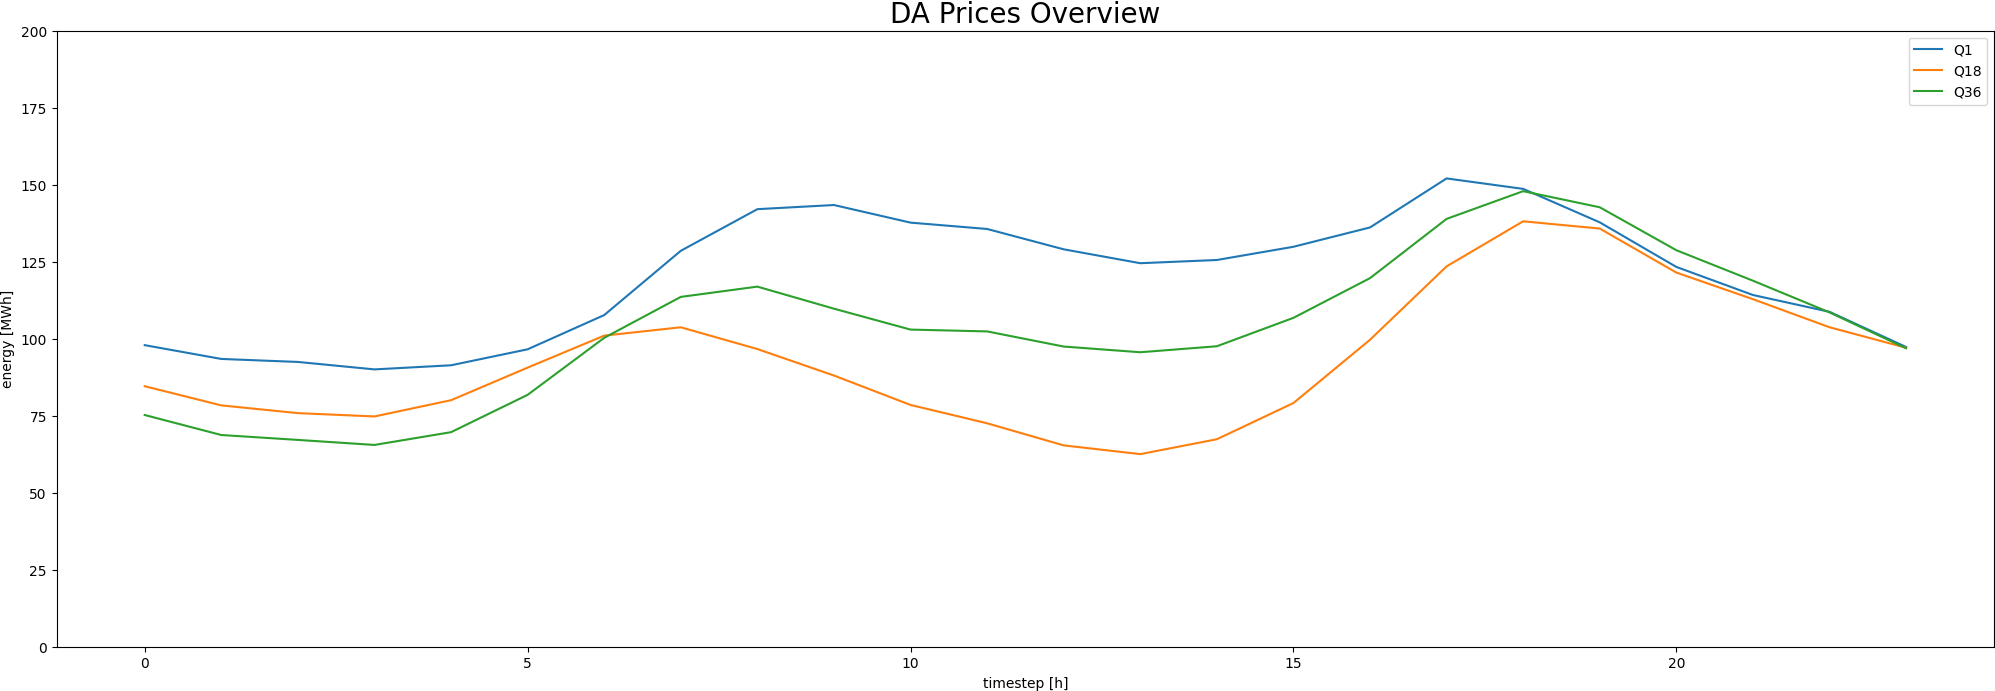
\includegraphics[width=1\linewidth]{pictures/results/DAPrices.png}
	\caption{DA Prices}
	\label{fig:DAPrices}
\end{figure}
\begin{figure}
	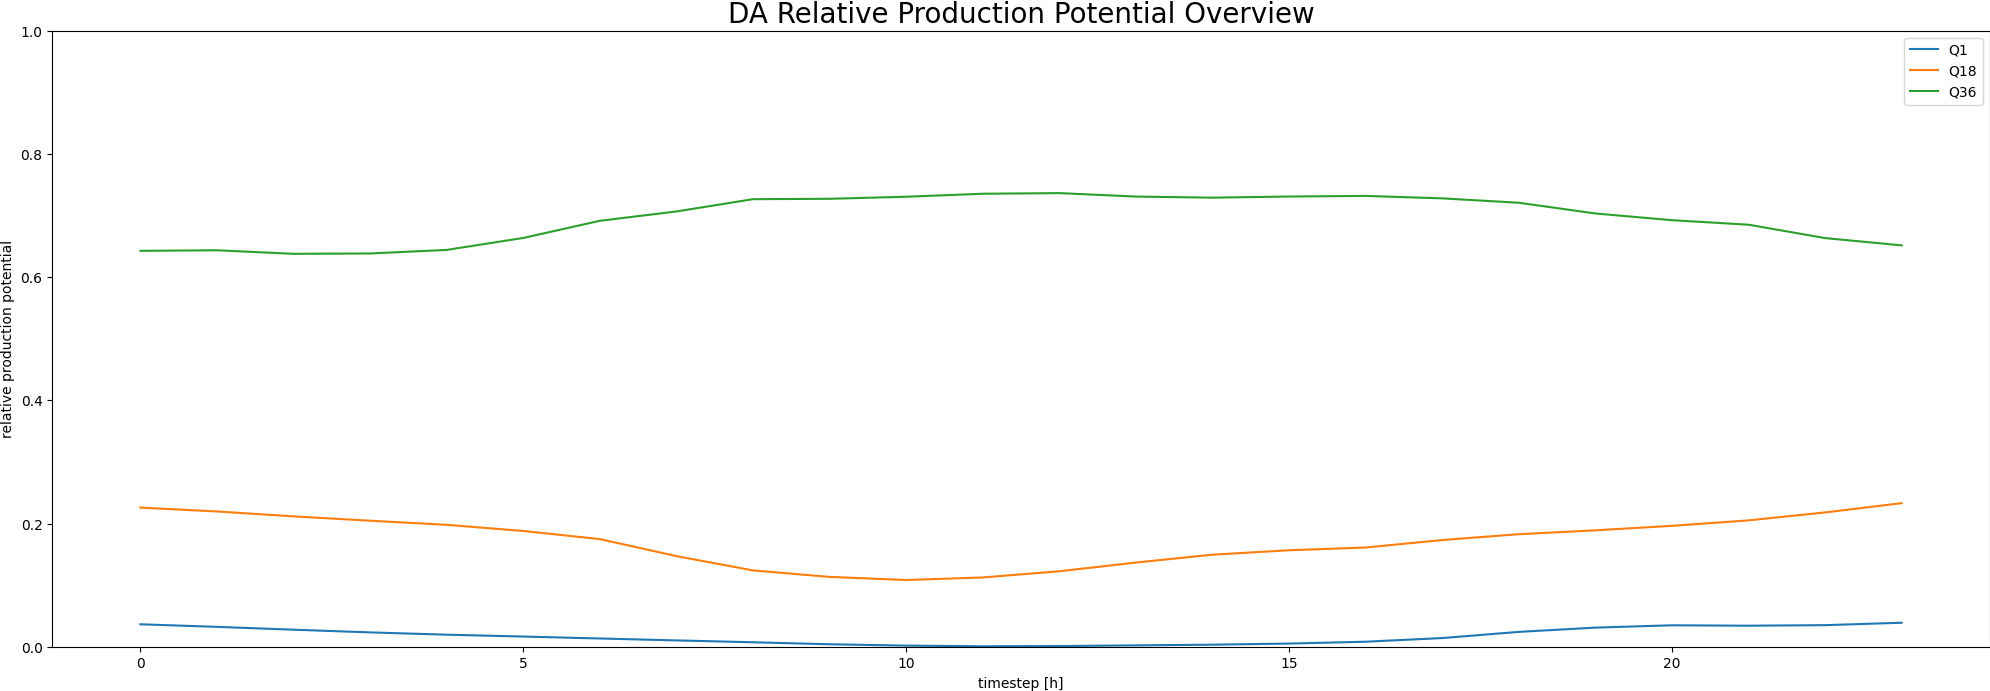
\includegraphics[width=1\linewidth]{pictures/results/DAProd.png}
	\caption{DA Production}
	\label{fig:DAProd}
\end{figure}

Außerdem stellt sich der entsprechende RL Markt wie folgt dar:

\begin{figure}[H]
	\centering
	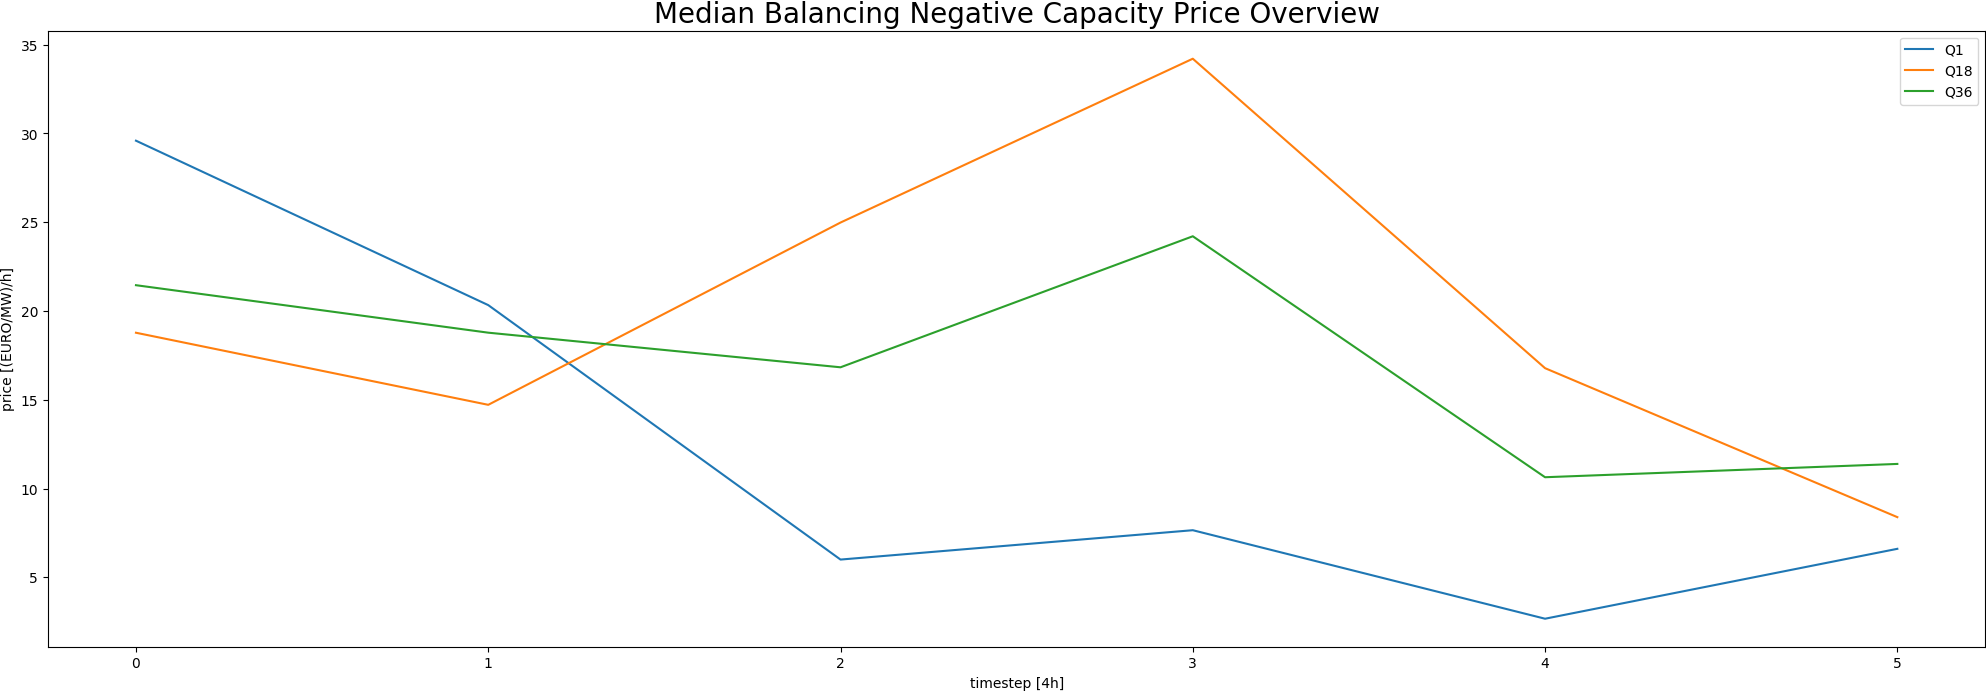
\includegraphics[width=1\linewidth]{pictures/results/RL_negPrice_Overview.png}
	\caption{RL Negative Prices}
	\label{fig:RL_negPrice_Overview}
\end{figure}
\begin{figure}
	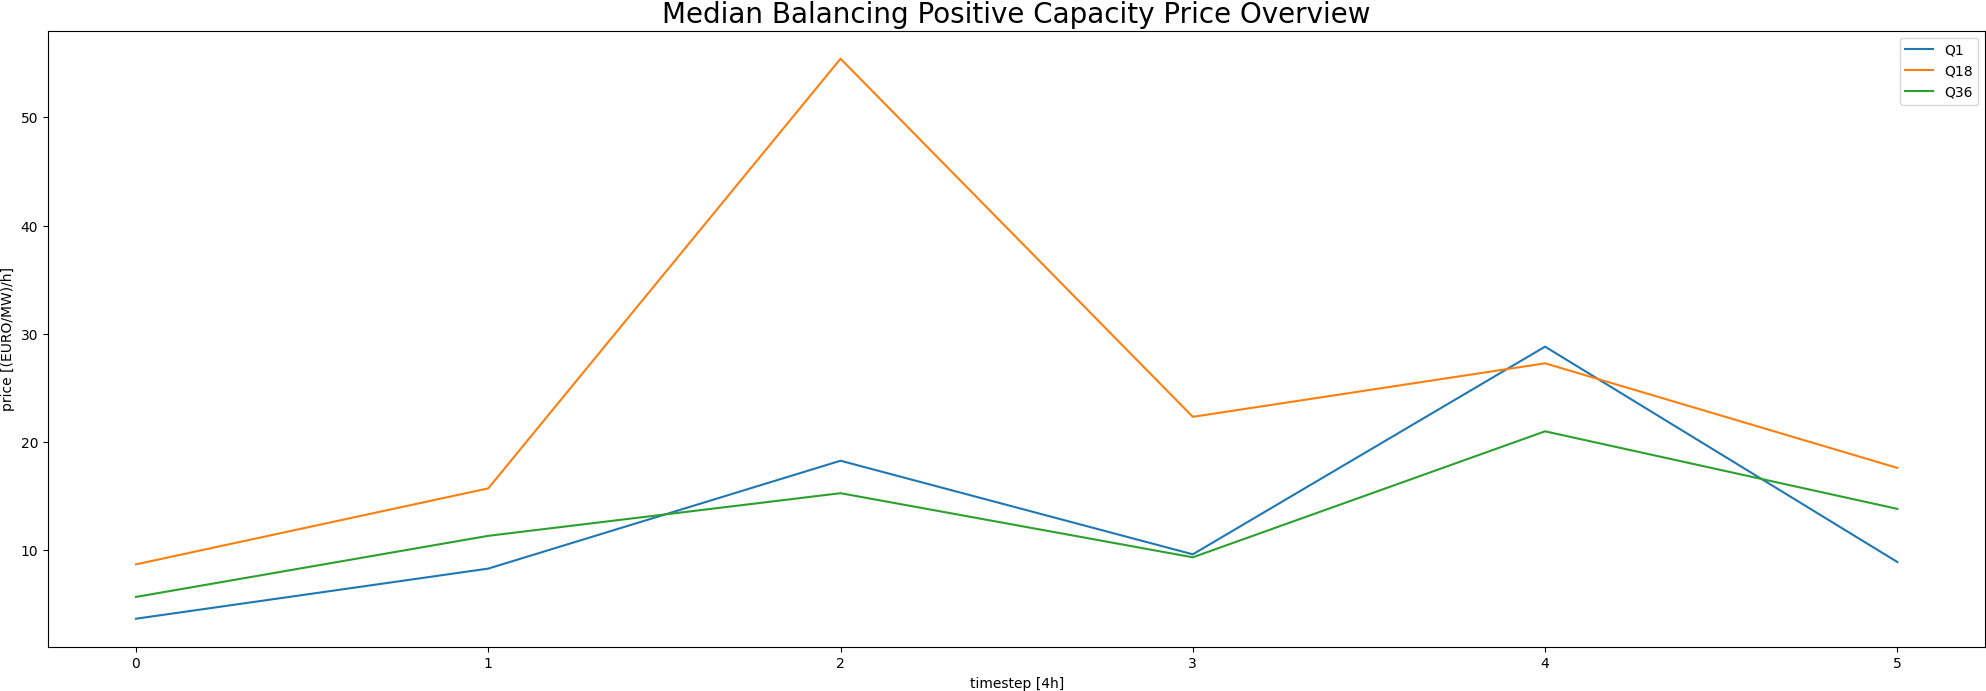
\includegraphics[width=1\linewidth]{pictures/results/RL_posPrice_Overview.png}
	\caption{RL Negative Prices}
	\label{fig:RL_posPrice_Overview}
\end{figure}

\section{Model Results}

\begin{figure}[H]
	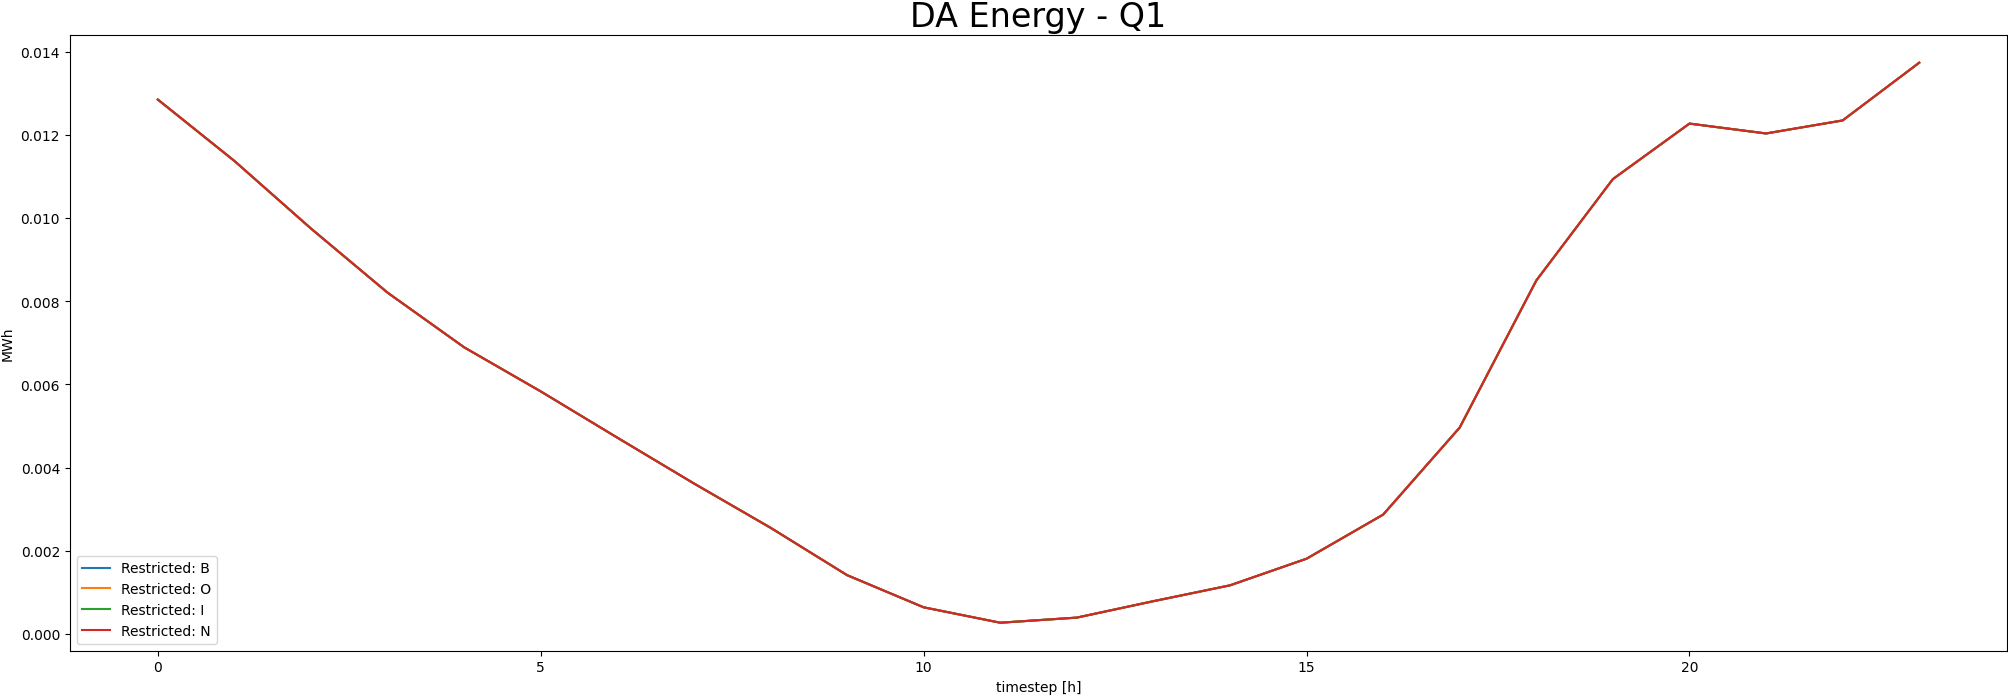
\includegraphics[width=1\linewidth]{pictures/results/DA Energy - Q1.png}
	\caption{DA Energy - Q1}
	\label{fig:DA Energy - Q1}
\end{figure}

\begin{figure}[H]
	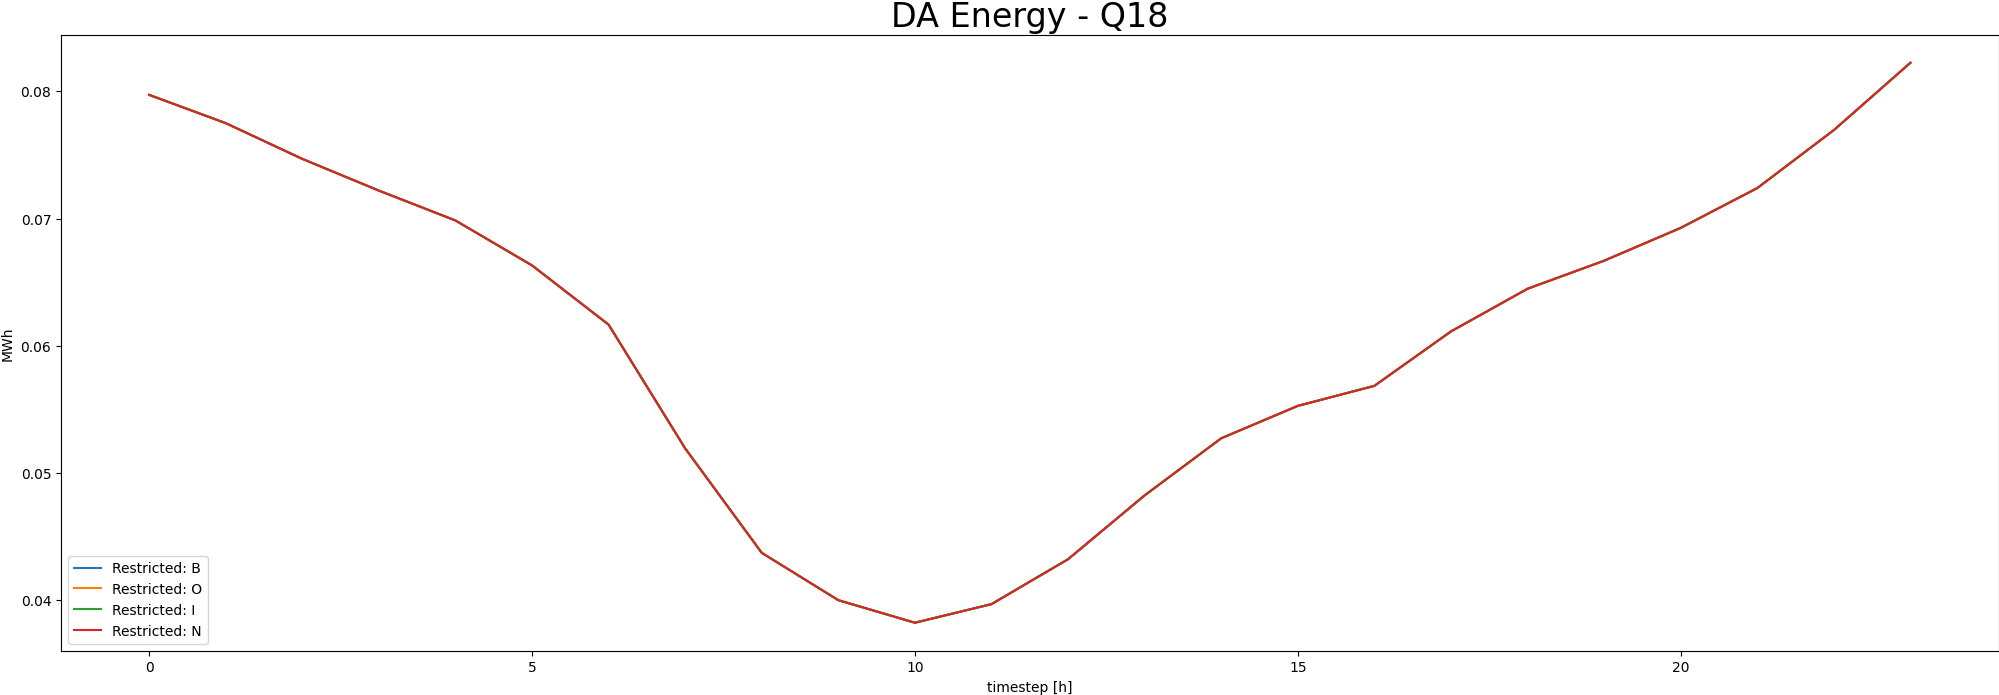
\includegraphics[width=1\linewidth]{pictures/results/DA Energy - Q18.png}
	\caption{DA Energy - Q18}
	\label{fig:DA Energy - Q18}
\end{figure}

\begin{figure}[H]
	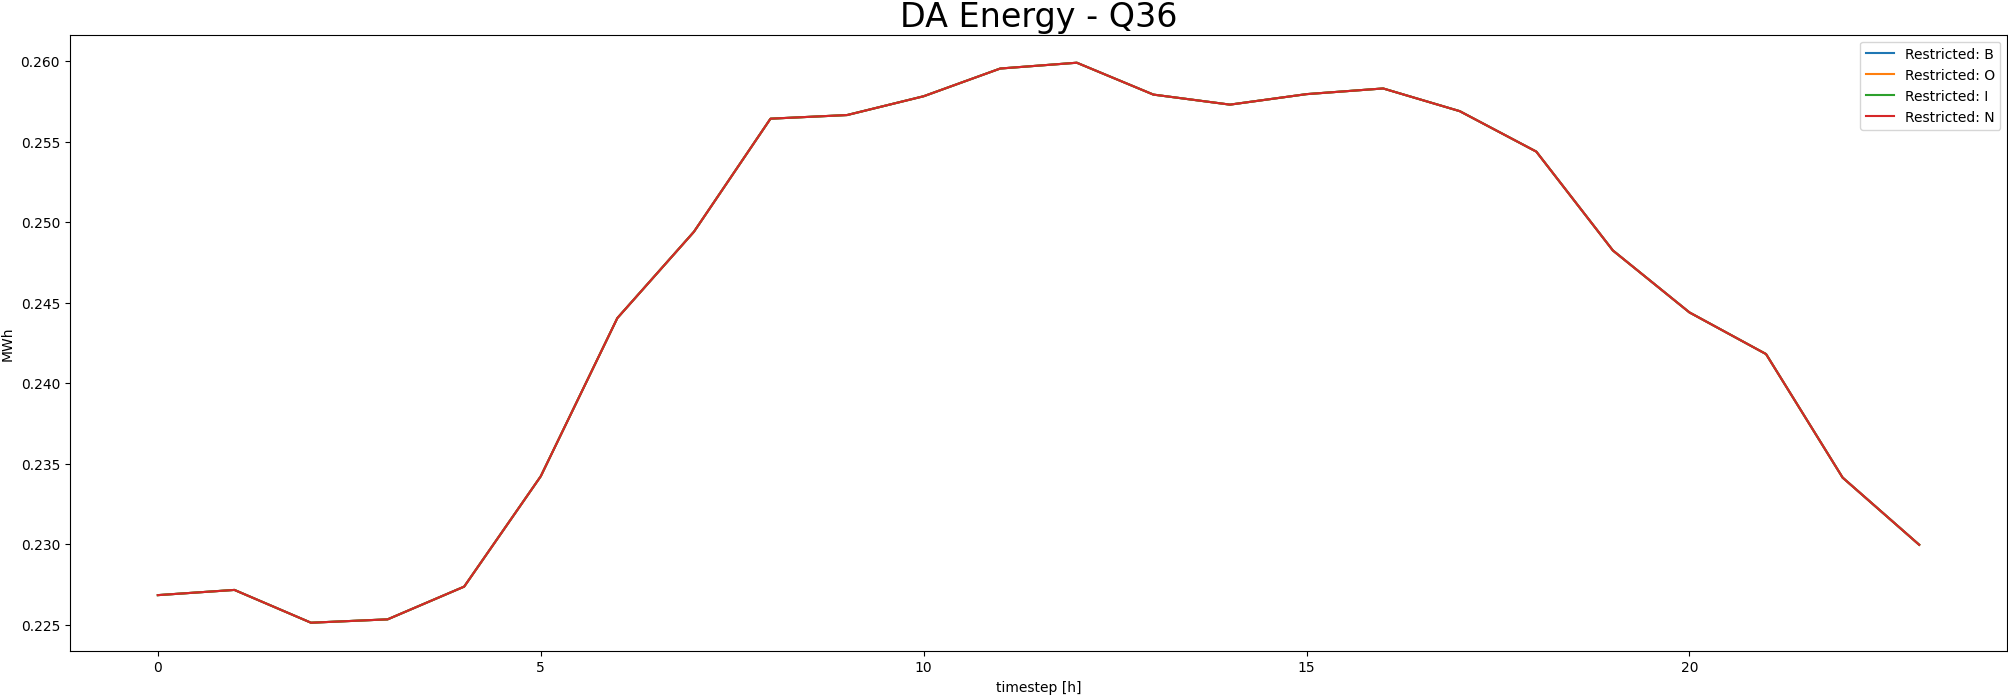
\includegraphics[width=1\linewidth]{pictures/results/DA Energy - Q36.png}
	\caption{DA Energy - Q36}
	\label{fig:DA Energy - Q36}
\end{figure}
\begin{figure}[H]
	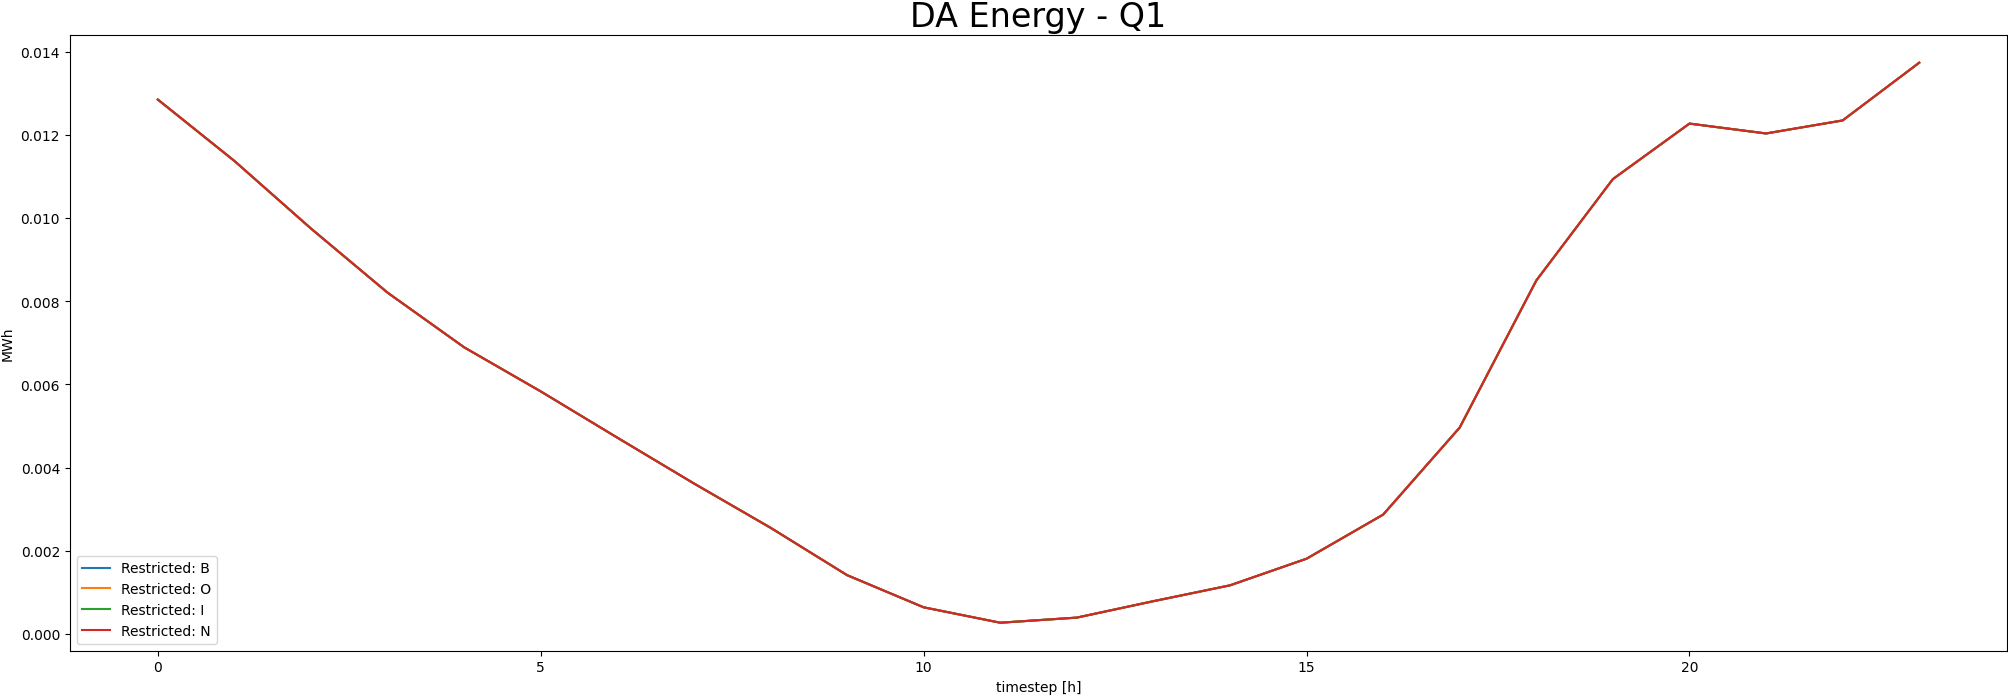
\includegraphics[width=1\linewidth]{pictures/results/DA Energy - Q1.png}
	\caption{Balance Capacity - Q1}
	\label{fig:Balance Capacity - Q1}
\end{figure}

\begin{figure}[H]
	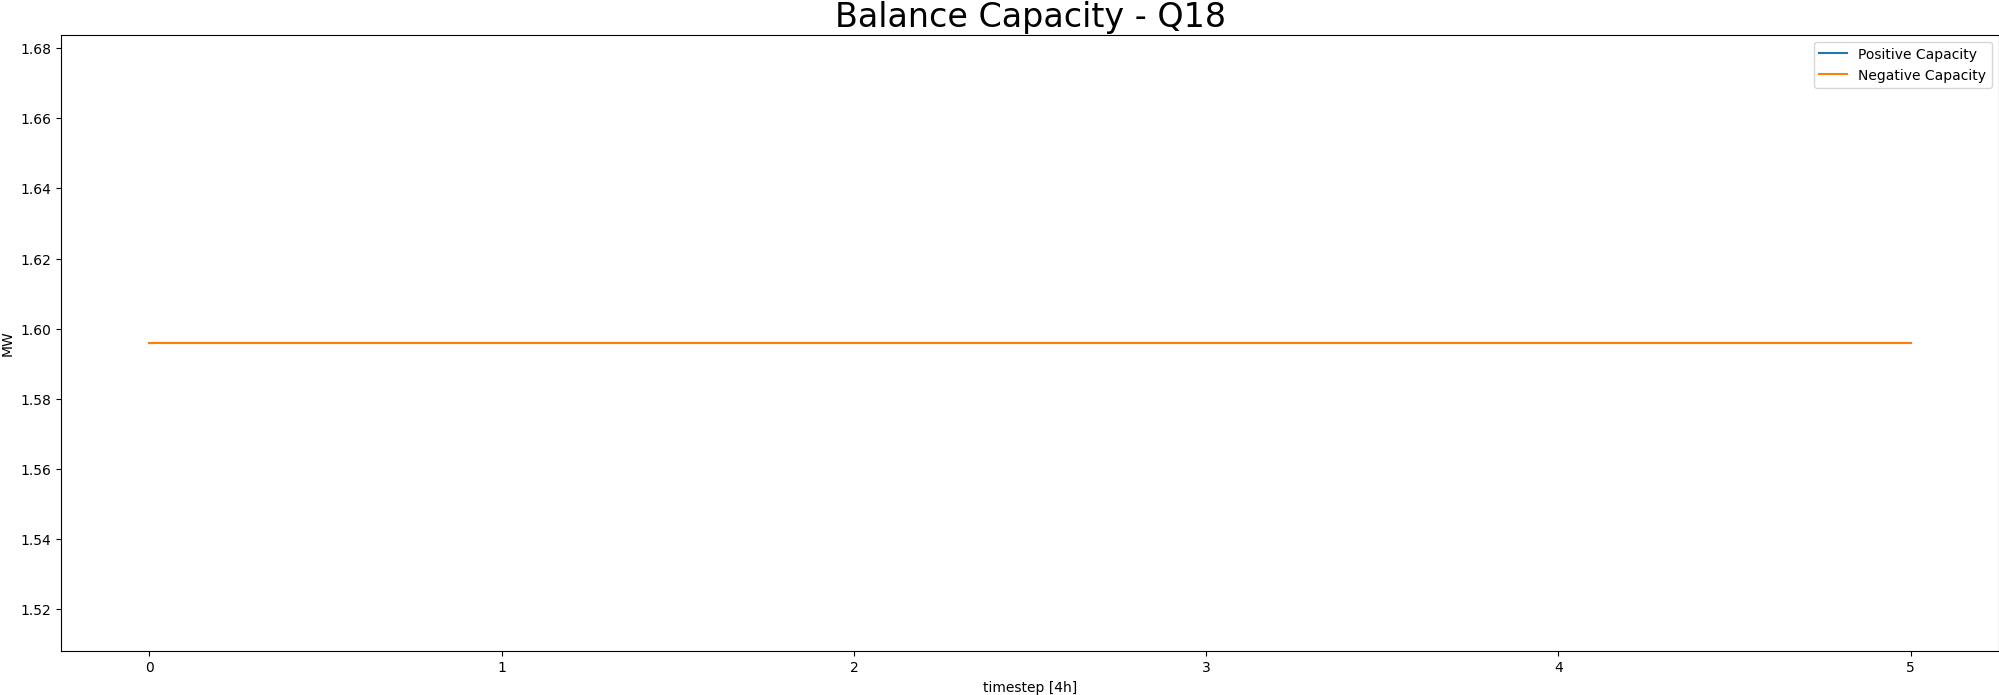
\includegraphics[width=1\linewidth]{pictures/results/Balance Capacity - Q18.png}
	\caption{Balance Capacity - Q18}
	\label{fig:Balance Capacity - Q18}
\end{figure}

\begin{figure}[H]
	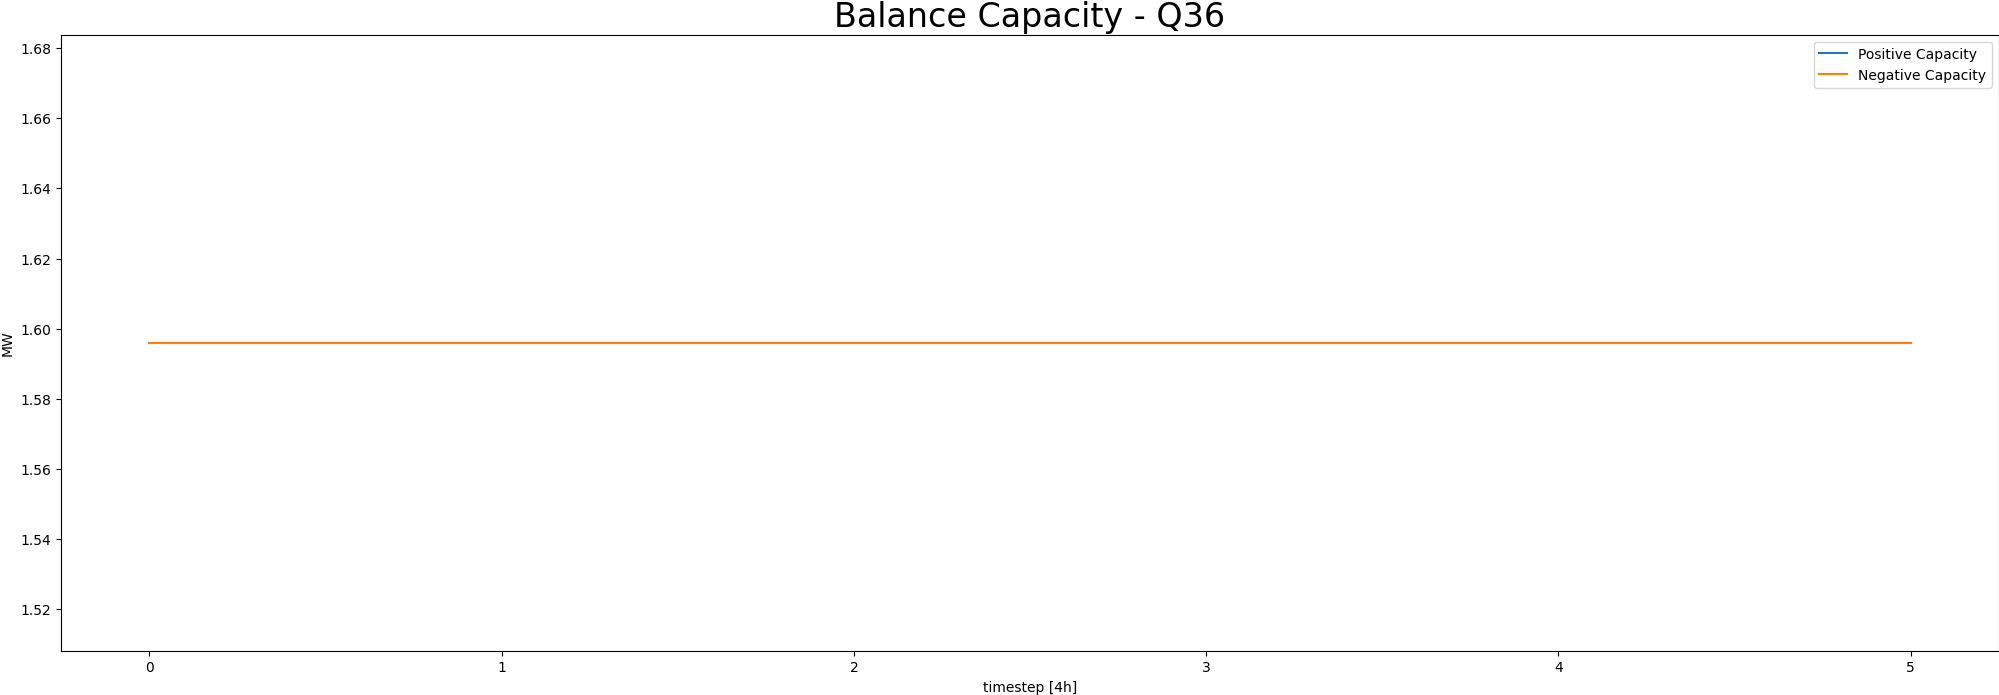
\includegraphics[width=1\linewidth]{pictures/results/Balance Capacity - Q36.png}
	\caption{Balance Capacity - Q36}
	\label{fig:Balance Capacity - Q36}
\end{figure}







\section{Digital Appendix}



%% *** local page settings ***
\addtocontents{toc}{\protect\setcounter{tocdepth}{+1}} %reset the decreased depth of the appendix entry in the ToC
\label{subsec:Bibliography}
\printbibliography[title={Bibliography}]
%% change chapter title to german if necessary



ChatGPT was utilized in this work for the following purposes:
\begin{itemize}
	\item As a search tool for specific functions.
	\item As an aid in refining formulations.
\end{itemize}
All suggestions were carefully reviewed and assessed individually.



\begin{center}
	\textbf{Statement of authorship}
\end{center}

I hereby certify that I have authored this document entitled "Model-based analysis of various
marketing options on the german secondary balancing market for a large-scale storage facility" independently
and without undue assistance from third parties. No other than the resources and references
indicated in this document have been used. I have marked both literal and accordingly adopted
quotations as such. There were no additional persons involved in the intellectual preparation
of the present document. I am aware that violations of this declaration may lead to subsequent
withdrawal of the academic degree.\\

\begin{figure}[!h]
	
\includegraphics[width=0.5\linewidth]{figures/unterschrift.png}
\end{figure}
Dresden, 20th April 2025\\
Sebastian Trümper\\




\end{document}
